%%%%%%%%%%%%%%%%%%%%%%% file template.tex %%%%%%%%%%%%%%%%%%%%%%%%%
%
% This is a general template file for the LaTeX package SVJour3
% for Springer journals.          Springer Heidelberg 2010/09/16
%
% Copy it to a new file with a new name and use it as the basis
% for your article. Delete % signs as needed.
%
% This template includes a few options for different layouts and
% content for various journals. Please consult a previous issue of
% your journal as needed.
%
%%%%%%%%%%%%%%%%%%%%%%%%%%%%%%%%%%%%%%%%%%%%%%%%%%%%%%%%%%%%%%%%%
%
\RequirePackage{fix-cm}
%
%\documentclass{svjour3}                     % onecolumn (standard format)
%\documentclass[smallcondensed]{svjour3}     % onecolumn (ditto)
\documentclass[smallextended]{svjour3}       % onecolumn (second format)
%\documentclass[twocolumn]{svjour3}          % twocolumn
%
\smartqed  % flush right qed marks, e.g. at end of proof
%
\usepackage{graphicx}
\usepackage{amsmath,amssymb,url,times}%,subfigure}% amsthm is the one!
\usepackage{caption,subcaption,hyperref}
\usepackage{color,comment}
\usepackage{curves,pgfgantt}
\usepackage[linesnumbered,ruled,vlined]{algorithm2e} 

% \usepackage{mathptmx}      % use Times fonts if available on your TeX system
%
% insert here the call for the packages your document requires
%\usepackage{latexsym}
% etc.
%
% please place your own definitions here and don't use \def but
% \newcommand{}{}
%
% Insert the name of "your journal" with
 \journalname{Journal of Intelligent \& Robotic Systems}

\newtheorem{prop}{Proposition}
\newcommand{\norm}[1]{\ensuremath{\left\| #1 \right\|}}
\newcommand{\abs}[1]{\ensuremath{\left| #1 \right|}}
\newcommand{\bracket}[1]{\ensuremath{\left[ #1 \right]}}
\newcommand{\braces}[1]{\ensuremath{\left\{ #1 \right\}}}
\newcommand{\parenth}[1]{\ensuremath{\left( #1 \right)}}
\newcommand{\ip}[1]{\ensuremath{\langle #1 \rangle}}
\newcommand{\refeqn}[1]{(\ref{eqn:#1})}
\newcommand{\reffig}[1]{Figure \ref{fig:#1}}
\newcommand{\tr}[1]{\mbox{tr}\ensuremath{\negthickspace\bracket{#1}}}
\newcommand{\trs}[1]{\mbox{tr}\ensuremath{\!\bracket{#1}}}
\newcommand{\deriv}[2]{\ensuremath{\frac{\partial #1}{\partial #2}}}
\newcommand{\G}{\ensuremath{\mathsf{G}}}
\newcommand{\SO}{\ensuremath{\mathsf{SO(3)}}}
\newcommand{\T}{\ensuremath{\mathsf{T}}}
\renewcommand{\L}{\ensuremath{\mathsf{L}}}
\newcommand{\so}{\ensuremath{\mathfrak{so}(3)}}
\newcommand{\SE}{\ensuremath{\mathsf{SE(3)}}}
\newcommand{\se}{\ensuremath{\mathfrak{se}(3)}}
\renewcommand{\Re}{\ensuremath{\mathbb{R}}}
\newcommand{\Sph}{\ensuremath{\mathsf{S}}}
\newcommand{\aSE}[2]{\ensuremath{\begin{bmatrix}#1&#2\\0&1\end{bmatrix}}}
\newcommand{\ase}[2]{\ensuremath{\begin{bmatrix}#1&#2\\0&0\end{bmatrix}}}
\newcommand{\D}{\ensuremath{\mathbf{D}}}
\renewcommand{\d}{\ensuremath{\mathbf{d}}}
\newcommand{\pair}[1]{\ensuremath{\left\langle #1 \right\rangle}}
\newcommand{\met}[1]{\ensuremath{\langle\!\langle #1 \rangle\!\rangle}}
\newcommand{\Ad}{\ensuremath{\mathrm{Ad}}}
\newcommand{\ad}{\ensuremath{\mathrm{ad}}}
\newcommand{\g}{\ensuremath{\mathfrak{g}}}
\newcommand{\argmin}{\operatornamewithlimits{argmin}}
\newcommand{\argmax}{\operatornamewithlimits{argmax}}
\graphicspath{{./Fig/}}
\newcommand{\WriteBlue}[1]{{\color{blue}\protect #1}}

\begin{document}

\title{Autonomous Exploration with Exact Inverse Sensor Models%Exact Occupancy Grid Mapping and Autonomous Exploration%\thanks{Grants or other notes
%about the article that should go on the front page should be
%placed here. General acknowledgments should be placed at the end of the article.}
}

%\titlerunning{Short form of title}        % if too long for running head

\author{Evan Kaufman \and Kuya Takami \and \\ Taeyoung Lee \and Zhuming Ai}%
%\thanks{Evan Kaufman, Taeyoung Lee, Mechanical and Aerospace Engineering, George Washington University, Washington DC 20052 {\tt \{evankaufman,tylee\}@gwu.edu}}
%\thanks{Zhuming Ai, Ira S. Moskowitz, Information Management \& Decision Architectures, U.S. Naval Research Laboratory,  Washington, DC 20375}
%}


%\authorrunning{Short form of author list} % if too long for running head

% Expanded:
\institute{E. Kaufman \at
              Dept. of Mechanical and Aerospace Engineering \\
		 The George Washington University \\
		 Washington DC 20052 \\
              Tel.: 216-346-0946\\
              \email{evankaufman@gwu.edu} 
           \and
           K. Takami \at
              Dept. of Mechanical and Aerospace Engineering \\
		 The George Washington University \\
		 Washington DC 20052 \\
              Tel.: 414-212-5155\\
              \email{kuya@gwu.edu} 
           \and
           T. Lee \at
              Dept. of Mechanical and Aerospace Engineering \\
		 The George Washington University \\
		 Washington DC 20052 \\
              Tel.: 202-994-8710\\
		 Fax: 202-994-0238\\
              \email{tylee@gwu.edu}
           \and
           Z. Ai \at
              Information Management \& Decision Architectures
              \\ U.S. Naval Research Laboratory \\
              Washington, DC 20375
}

% Condensed:
\institute{E. Kaufman, K. Takami, and T. Lee \at
              Dept. of Mechanical and Aerospace Engineering \\
		 The George Washington University \\
		 Washington DC 20052 \\
              Tel.: 202-994-8710\\
              \email{\{evankaufman,kuya,tylee\}@gwu.edu} 
           \and
           Z. Ai \at
              Information Management \& Decision Architectures
              \\ U.S. Naval Research Laboratory \\
              Washington, DC 20375
}




\date{Received: date / Accepted: date}
% The correct dates will be entered by the editor


\maketitle

\begin{abstract}
This paper is focused on probabilistic occupancy grid mapping and motion planning such that a robot may build a map and explore a target area autonomously in real time. The desired path of the robot is developed in an optimal fashion to maximize the information gain from the sensor measurements on its path, thereby increasing the accuracy and efficiency of mapping, while explicitly considering the sensor limitations such as the maximum sensing range and viewing angle. 
Most current exploration techniques require frequent human intervention, often developed for omnidirectional sensors with infinite range.
The proposed research is based on realistic assumptions on sensor capabilities. The unique contribution is that the mapping and autonomous exploration techniques are systematically developed in a rigorous, probabilistic formulation. The mapping approach exploits the probabilistic properties of the sensor and map explicitly, and the autonomous exploration is designed to maximize the expected map information gain, thereby improving the efficiency of the mapping procedure and the quality of the map substantially. The efficacy of the proposed optimal approach is illustrated by both numerical simulations and experimental results. 
%%%% Before minor modifications restructuring the abstract by Evan Kaufman on October 14, 2016:
%This paper is focused on probabilistic occupancy grid mapping and motion planning such that a robot may build a map and explore a target area autonomously in real time. The desired path of the robot is developed in an optimal fashion to maximize the information gain from the sensor measurements on its path, thereby increasing the accuracy and efficiency of mapping, while explicitly considering the sensor limitations such as the maximum sensing range and viewing angle. Most current exploration techniques require frequent human intervention, and they are frequently developed for omnidirectional sensors with infinite range. 
%%For example, when applying SLAM techniques to explore an unknown area, a human operator must provide the path of the vehicle while continuously monitoring the updated map. 
%The proposed research will greatly improve autonomy of robotic exploration in a systematic optimal manner, under realistic assumptions on sensor capabilities. The unique contribution is that the mapping and autonomous exploration techniques are systematically developed in a rigorous, probabilistic formulation. The mapping approach exploits the probabilistic properties of the sensor and map explicitly, and the autonomous exploration is designed to maximize the expected map information gain, thereby improving the efficiency of the mapping procedure and the quality of the map substantially. The efficacy of the proposed approach is illustrated by both numerical simulations and experimental results. 
\keywords{Occupancy Grid Mapping \and Inverse Sensor Model \and Autonomous Exploration}
% \PACS{PACS code1 \and PACS code2 \and more}
% \subclass{MSC code1 \and MSC code2 \and more}
\end{abstract}

\section{Introduction}
\label{intro}
Robotic mapping is the process of generating maps, which represent the environment in close proximity of a robot. 
%Mapping in the context of robotics is to generate maps, which represent the environment in close proximity of a robot. 
This problem is crucial to understanding the surrounding regions when a robot enters an uncertain environment.
Various map representations include occupancy grids~\cite{WolSuk05}, octomaps~\cite{WurHorBenStaBur10}, or feature-based maps%in a landmark representation
~\cite{MonThrKolWeg02}.
%To build maps in real time, a computationally-efficient algorithm is required.% \EditTL{rewrite this paragraph for mapping, without introducing SLAM here}

For mobile robots to operate in an unknown environment autonomously, they should be able to construct a map of the environment by using onboard sensors, and estimate their position in the constructed map. Simultaneous localization and mapping problem (SLAM) serves to estimate the map of the environment and the pose of robots concurrently, and there have been various approaches developed for SLAM with successful demonstrations.

However, there are certain issues with the current SLAM techniques. First, the vast majority of work deals only with the aspect of estimating the environment and the poses of vehicles. They are passive in the sense that SLAM is performed on incoming sensor measurements from vehicles following an arbitrary path. As such, human teleoperation and monitoring are often essential to guide the vehicles safely through unknown surroundings. Therefore, it is desired that an active motion planning scheme is developed and integrated with SLAM such that vehicles are able to determine their path without human intervention, and explore unknown areas autonomously.

To achieve these, it is proposed that the problems of mapping and motion planning are integrated in a probabilistic formulation. More explicitly, the map is constructed in a probabilistic sense, in contrast to the common approaches where the map is defined by deterministic objects that are definitely occupied or free. One of the desirable features for the proposed stochastic formulation is that we can extract the information on the degree of uncertainty for the each part of the map, such that the motion of the vehicle is planned to minimize the map uncertainty in an optimal fashion. 

This is addressed in two steps. The first part of this paper focuses on probabilistic occupancy grid mapping given a stochastic model of a range sensor, and the second part deals with stochastic motion planning to construct optimal exploration strategies. 

\paragraph{Probabilistic Occupancy Grid Mapping}

The proposed approach is based  on the occupancy grid representation, where the environment is decomposed into evenly-spaced grid cells, considered as either occupied or free. The probabilistic model of a range sensor is referred to as the \textit{forward sensor model}, which provides a probability of range measurements for the given pose of the vehicle and the exact map~\cite{ThrBurFox05}. One can characterize the performance of a range sensor, such as its accuracy or maximum range, completely with its forward sensor model. 

The mapping problem can be defined as finding the \emph{inverse sensor model}, which is the probability of occupancy for a grid cell based on range measurements and the configuration of the mobile robot, which is of fundamental importance with occupancy grid mapping. However, the exact solution to the inverse sensor model has not been utilized in occupancy grid mapping, because the computational requirements are too cumbersome to compute the exact model in real time~\cite{ThrBurFox05}.

Instead, several techniques have been proposed to approximate the exact inverse sensor model. %Due to the computational limitations, two common approaches are applied to obtain a function close to the inverse sensor model.
In the early occupancy grid mapping applications based on sonar sensors, \emph{ad hoc} techniques to obtain an inverse sensor model were developed based off highly-innacurate bouncing sound waves~\cite{MorElf85,Elf89}.
%These occupancy grid mapping schemes employ \emph{ad hoc} techniques to obtain the inverse sensor model.
These techniques rely on approximate functions to represent the inverse sensor model with questionable accuracy~\cite{ChoLynHutKanBurKavThr05} and applied to more modern sensors in~\cite{And09},~\cite{PirRutBisSch11}.

The other popular approach to obtain an approximate inverse sensor model is to simulate maps, robot poses, and measurements and use a learning algorithm to approximate the inverse sensor model~\cite{ThrBurFox05,Thr01}. These approaches are undesirable in practice due to complexities associated with implementing a learning algorithm. For example, the accuracy of such inverse sensor models strongly depends on the samples selected for learning, but it is unclear how to select those samples, or how many samples are required to obtain a reasonable approximation. Furthermore, it is challenging to apply any learning algorithm over the large dimensional space composed of maps, poses, and measurements. 

%and they only yield probabilistic approximations without strong mathematical justification. 

%These approaches simply treat occlusions with discrete probabilities of detection, regardless of whether one cell may completely, partially, or not block another cell in the sensor field of view.

%Furthermore, both approaches follow a log-odds ratio Bayesian framework, imposing an additional Markov assumption.

%These techniques are not also suitable for modern range sensor with the highly accurate bearing~\cite{Thr03}. Based on recent improvements in sensor technology, the occupancy grid mapping problem has been restructured using the fact that depth measurement bearings are known. \EditTL{do we need this paragraph?}

This paper proposes a computationally efficient algorithm to construct the exact inverse sensor model. More explicitly, for a given forward sensor model defined by the probability distribution of range measurements, this algorithm yields the a posteriori probabilities of occupancy of all the cells within the area covered by the range sensor from the range measurements. The key idea is reducing the computational load by using the fact that if a cell is occupied, the occupancies of the other cells blocked by it is irrelevant to the forward sensor model, and this property is systematically utilized with various probabilistic properties to derive a computationally-efficient solution to the inverse sensor model. Furthermore, the proposed approach integrates a priori probabilities of occupancy and multiple range measurements according to the Bayesian framework to obtain more accurate maps. As such, it contrasts from the existing framework based on log-odds ratios that impose an additional Markov assumption. 

\paragraph{Optimal Autonomous Exploration}

Next, this paper addresses autonomous exploration to plan the trajectories of the vehicle to generate a complete, accurate map~\cite{Yam97}. We present an approach where the robot chooses a trajectory designed to maximize information gain of the occupancy grid map.

%Another major problem that this paper addresses is to determine an effective trajectory given little knowledge about the environment.  Autonomous exploration solves this problem, by choosing robotic motion through uncertain space, while building a map that is used for subsequent navigation~\cite{Yam97}.

A common approach to solve the autonomous exploration problem is known as frontier-based exploration, such as ~\cite{Yam97,Yam98}. This is the process of executing actions that move the robot toward the closest boundary between visited and unvisited space, known as a frontier.
Then the robot takes measurements at this location such that the mapped territory expands, and thus the new frontiers are pushed back. This process is repeated until the map is well-known.
Frontier-based exploration assumes that repeatedly moving toward the closest frontier and taking measurements are the best actions to gain new information about the map, though these systematic actions are not based on any consideration of the future uncertainty of the probabilistic map or optimality.
%there is no guarantee that these actions satisfy any optimality criteria.

%The uncertainty of an occupancy grid map is commonly measured with Shannon's entropy, which is a metric that measures map uncertainty.

%Approaches aimed at determining the future uncertainty of an occupancy grid map commonly suffer from several approximations.
%%Determining future occupancy grid map uncertainty requires predictive estimations, which suffer from several approximations. 
%Most evident is that all approaches rely on inaccurate probabilistic occupancy grids. This mapping representation is typically based on heuristic approximations (e.g.~\cite{MorElf85,Elf89,ChoLynHutKanBurKavThr05,And09,PirRutBisSch11}) or simulated learning techniques \cite{ThrBurFox05,Thr01}. Map-based information gain is commonly determined with Shannon's entropy~\cite{CarDamKumCas15}, an uncertainty metric based on grid cell occupancy probability. Since this probability is heuristic or learned, any measure of entropy is subject to errors from approximated probability.
%Furthermore, the expected entropy of an action is not directly calculated~\cite{CarDamKumCas15,StaGriBur05}. Instead, these particle filter-based approaches assume that expected entropy is equivalent to entropy based on expected measurement scans~\cite{JohStaPfaBur07}. This assumption is subject to inaccuracies due to the nonlinear nature of Shannon's entropy. %Furthermore, these approaches typically generate maps with a particle filter, which commonly require some tuning and may consume large amounts of onboard memory.
%
%In this paper, we propose an autonomous exploration technique based on expected entropy change that avoids the aforementioned issues. 
%%The occupancy grid mapping scheme is based on~\cite{KauLeeAiMos16}, which provides the exact solution of occupancy grid mapping of a single measurement ray. 
%We develop a solution for expected entropy gain based on exact occupancy grid mapping~\cite{KauLeeAiMos16}. This solution directly calculates expected entropy from a probabilistic map based on similar assumptions of those applied to occupancy grid mapping.
%Though more accurate than several other approaches, the proposed solution requires large computational resources, making real-time implementation difficult in certain scenarios.
%Thus, we provide the tools to approximate the exact solution that reduce the computational requirements with realistic assumptions.
%The motion of the robot is formulated as an optimization problem, where the expected entropy change is minimized, or equivalently the expected information gain is maximized.

Alternatively, there have been exploration techniques that are based on a quantitative measure of uncertainty. However, these approaches commonly suffer from several approximations. Most evident is that all approaches rely on inaccurate probabilistic occupancy grids. 
This mapping representation is typically based on heuristic approximations (e.g.~\cite{MorElf85,Elf89,ChoLynHutKanBurKavThr05,And09,PirRutBisSch11}) or simulated learning techniques \cite{ThrBurFox05,Thr01}. Map-based information gain is commonly determined with Shannon's entropy~\cite{StaGriBur05}, an uncertainty metric based on grid cell occupancy probability. Since this probability is heuristic or learned, any measure of entropy is subject to errors from approximated probability or ad hoc learning.
Furthermore, the expected entropy of an action is not directly calculated. Instead, these particle filter-based approaches assume that expected entropy is equivalent to entropy based on expected measurement scans~\cite{JohStaPfaBur07}. This assumption is subject to inaccuracies due to the nonlinear nature of Shannon's entropy. For these reasons, more careful computation of map uncertainty is warranted. %Furthermore, these approaches typically generate maps with a particle filter, which commonly require some tuning and may consume large amounts of onboard memory.

In this paper, we propose an autonomous exploration technique based on expected entropy change that avoids the aforementioned issues. 
%The occupancy grid mapping scheme is based on~\cite{KauLeeAiMos16}, which provides the exact solution of occupancy grid mapping of a single measurement ray. 
We develop a solution for expected entropy gain based on exact occupancy grid mapping~\cite{KauLeeAiMos16}. This solution directly calculates expected entropy from a probabilistic map based on similar assumptions of those applied to occupancy grid mapping.
Though more accurate than several other approaches, the proposed solution requires large computational resources, making real-time implementation difficult in certain scenarios.
Thus, we provide the tools to approximate the exact solution that reduces the computational requirements with realistic assumptions.
The motion of the robot is formulated as an optimization problem, where the expected entropy change is minimized, or equivalently the expected information gain is maximized.
Compared with the recent results (e.g. [12], [13], [16], [17]) that employ Rao-Blackwellized particle filters to deal with localization and autonomous exploration simultaneously with an approximate entropy change, this paper is based on an accurate probabilistic solution to map information gain, under the assumption that the robot pose is known. Accounting for the stochastic properties of position and attitude is important to the field of robotics, and accounting for localization in conjunction with mapping and exploration are considered as a future step to this paper.

In short, the main contribution of this paper is proposing the exact inverse sensor model and constructing an exact Bayesian occupancy grid mapping based on that. Compared with the current mapping algorithms based on an approximate inverse sensor model, this approach yields more accurate occupancy probabilities. This constructs substantially more accurate occupancy grid maps with less uncertainty for the same set of measurements, and these are directly illustrated by numerical examples and experimental results. Additionally, we derive a computationally-efficient approach to predict map information gain for autonomous exploration with a novel structure that avoids several common assumptions and approximations. By computing the expected information precisely with the exact inverse sensor model, the proposed autonomous exploration approach constructs a more accurate map with limited sensor capabilities in an optimal fashion. While this paper is focused on mapping and exploration in two-dimensional environments, the presented results can be certainly utilized in SLAM or stochastic motion planning in three dimensions.









\section{Problem Formulation}
\label{sec:ProbForm}

\subsection{Probabilistic Occupancy Grid Mapping}
\label{subsec:POGM}
Let a map $m$ be decomposed into $n_m$ evenly-spaced grid cells, where the $i$-th grid cell is assigned to a static binary random variable $\mathbf{m}_i$ for $i\in\braces{1,2,\ldots,n_m}$, that is defined as $\mathbf{m}_i=1$ when occupied, and $\mathbf{m}_i=0$ when free. The location and size of each grid cell is assumed known, where a smaller cell size (greater grid resolution) better represents a space, but increases computation and memory. Therefore, a map $m$ is defined by $\{\mathbf{m}_1,\ldots, \mathbf{m}_{n_m}\}$ ($2^{n_{m}}$ possible maps).

Another random variable is defined as $\bar{\mathbf{m}}_i=1-\mathbf{m}_i$ for convenience. The probability that the $i$-th cell is occupied is $P(\mathbf{m}_i)$, and the probability that it is free is $P(\bar{\mathbf{m}}_i)=1-P(\mathbf{m}_i)$. The random variables $\mathbf{m}_i$ are mutually independent, 
\begin{align}
P(m)=P(\mathbf{m}_1,\mathbf{m}_2,\ldots,\mathbf{m}_{n_m})=\prod_{i=1}^{n_m}P(\mathbf{m}_i).
\end{align}

Consider a range sensor that provides scans of the surrounding environment in order to identify the closest occupied space. The location and the direction of the sensor, referred to as the \emph{pose} at time $t$, is denoted by $X_t=(x_t,R_t)$, where the planar position and direction of the robot at $t$ are denoted by $x_t\in\Re^2$ and $R_t\in\Sph^1=\braces{q\in\Re^2|\norm{q}=1}$, i.e., the attitude corresponds to a direction on a 2D plane.  Let $X_{1:t}$ denote the history of poses from the initial time to the current time, i.e., $X_{1:t}=\{X_1,X_2,\ldots, X_t\}$. At each pose, the robot receives a 2D measurement \emph{scan}, composed of $n_z$ measurement \emph{rays}. These rays are 1D depth measurements of known direction from the current pose to the closest occupied space, subject to a known \emph{forward sensor model} $p(z_{t,l}|m,X_t)$, where $z_{t,l}$ is the $l$-th measurement ray of the $t$-th scan $Z_t=\braces{z_{t,1},z_{t,2},\ldots,z_{t,n_z}}$. The measurement history is denoted by $Z_{1:t}=\braces{Z_1,Z_2,\ldots,Z_t}$. 

The probability density function, namely $p(z_{t,l}|m,X_t)$ with respect to the depth of the $l$-th measurement ray conditioned on the map $m$ and the pose $X_t$ is commonly referred to as the \emph{forward sensor model}, which characterizes the corresponding depth sensor, such as the maximum range or accuracy. The forward sensor model satisfies  (i) the ranges of all depth measurements are positive and finite, and (ii) measurement rays cannot pass through occupied regions. Throughout this paper, we assume that the forward sensor model of the selected sensor is given. This can be determined empirically or analytically. For example, the \emph{beam model for range finders} satisfying  the above criteria is described in~\cite{ThrBurFox05}.


Occupancy grid mapping provides occupancy probabilities based on robot poses and measurement scans. The goal is to obtain $P(\mathbf{m}_i|X_{1:t},Z_{1:t})$, commonly referred to as the \emph{inverse sensor model} for given forward sensor model $p(z_{t,l}|m,X_t)$ and the initial estimate of the map $P(m)$ with $X_{1:t}$ and $Z_{1:t}$.







\subsection{Autonomous Exploration}
\label{subsec:AE}
Since occupancy grid mapping provides a probabilistic representation of surrounding space, this mapping scheme holds probabilistic information about the uncertainty of the map. Shannon's entropy is commonly used as a measure of uncertainty, such as in~\cite{StaGriBur05}. Given the probabilities of each grid cell of map $m$, Shannon's entropy is defined as the sum of the entropy of each cell,
\begin{align}
\label{eqn:ShannonsEntropyDef}
H(&P(m))=%\nonumber\\&
-\sum_{i=1}^{n_m}\braces{
P(\mathbf{m}_i)\log{P(\mathbf{m}_i})+P(\bar{\mathbf{m}}_i)\log{(P(\bar{\mathbf{m}}_i}))}.
\end{align}
The entropy of the $i$-th grid cell is maximized when $P(\mathbf{m}_i)=0.5$ (greatest uncertainty) and minimized when $P(\mathbf{m}_i)\in\braces{0,1}$ (smallest uncertainty). %; thus Shannon's entropy is a measure of uncertainty.

The goal of autonomous exploration is to determine future poses that maximize the map information gain, or equivalently minimize the map entropy. 
Since autonomous exploration is conducted in uncertain environments, a complete trajectory cannot be known before the robot takes measurements of the entire reachable space.
Instead, an objective function governs the motion between intermediate poses, building an occupancy grid map along the way.

Suppose at time $t$, $P(m|X_{1:t},Z_{1:t})$ is given. Let $X_c$ be a candidate pose under consideration for some future time step.
The expected information gain $\mathcal I(X_c)$ is defined as the negative change of entropy
\begin{align}
\label{eqn:ObjFun}
\mathcal I(X_c)&=H(P(m|X_{1:t},Z_{1:t}))%\nonumber\\&\quad
-\text{E}\left[H(P(m|X_{1:t},Z_{1:t},X_c,Z_c))\right],
\end{align}
where $H(P(m|X_{1:t},Z_{1:t}))$ may be computed with \refeqn{ShannonsEntropyDef} and \\$\text{E}\left[H(P(m|X_{1:t},Z_{1:t},X_c,Z_c))\right]$ is the expected entropy when the robot is located at $X_c$, where the expectation is taken over $Z_c$.
Since autonomous exploration is formulated as a trajectory optimization, the goal is to repeatedly choose optimal $X_c^*$ that maximizes the objective function
\begin{align}
\label{eqn:Objective}
X_c^*=\argmax_{X_c}{\mathcal I(X_c)},
\end{align}
where $X_c^*$ satisfies the inequality constraint to avoid collisions,
\begin{align}
\label{eqn:CollisionInequalityConstraint}
P_\text{collision}(X)=1-\prod_{i\in\mathcal C_X}P(\bar{\mathbf{m}}_i|X_{1:t},Z_{1:t})\leq\beta,
\end{align}
where $\mathcal C_X$ is the set of grid cells falling inside a volume of preselected size around $X$ that may cause collision and $\beta>0$ is a threshold of the probability of collision. It is considered that once a collision-free trajectory toward $X_c^*$ is obtained, the robot moves along the trajectory controlled by a motion control system in the inner loop. Once the robot has translated to $X_c^*$, the above process is repeated.








\section{Occupancy Grid Mapping with an Exact Inverse Sensor Model}
\label{sec:ISM}

This section outlines issues with the common log-odds ratio formulation and perceived computational burdens with the exact solution to the inverse sensor model for occupancy grid mapping. Then, a method that exploits several mapping and probabilistic properties provides a computationally efficient exact solution to probabilistic occupancy grid mapping.

\subsection{Mapping via Log-Odds Ratio}

One of the popular frameworks of updating binary random variables with static state is with a binary Bayesian filter using the log-odds ratio formulation.
The main idea is that instead of multiplying terms from prior and current time steps, the properties of logarithms allow these terms to be simply added, while avoiding truncation issues associated with probabilities close to $0$ or $1$~\cite{ThrBurFox05}.
The log-odds ratio is also popular because learning techniques with forward models~\cite{Thr01},~\cite{Thr03} or ad hoc techniques~\cite{MorElf85},~\cite{Elf89} become simplified.%are simpler to derive when they need not consider $P(\mathbf{m}_i|X_{1:t},Z_{1:t-1})$ as part of the inverse sensor model, but rather only $P(\mathbf{m}_i)$, which is typically fixed and uniform for all cells.

However, the log-odds ratio formulation makes an assumption that is not consistent with the occupancy grid mapping problem. It is assumed that if $X_t$ and $\mathbf{m}_i$ are known, then $Z_t$ is independent of $X_{1:t-1}$ and $Z_{1:t-1}$, i.e.,
%\begin{align}
%\label{eqn:FirstBayesRule}
%P(\mathbf{m}_i|X_{1:t},Z_{1:t})
%&
%=\frac{P(Z_t|\mathbf{m}_i,X_{1:t},Z_{1:t-1})P(\mathbf{m}_i|X_{1:t},Z_{1:t-1})}{P(Z_t|X_{1:t},Z_{1:t-1})}.
%\end{align}
\begin{align}
\label{eqn:AssumptionEarly}
P(Z_t|\mathbf{m}_i,X_{1:t},Z_{1:t-1})\approx P(Z_t|\mathbf{m}_i,X_t).
\end{align}
In other words, the past history of measurements and poses are irrelevant to the current measurement. However, the prior measurements and poses provide a certain information to the occupancy map, which affects the probabilistic model of the current measurement. 

More specifically, forward models are based on the entire map $m$. Since \refeqn{AssumptionEarly} conditioned only by the $i$-th cell, past poses $X_{1:t-1}$ and past measurement scans $Z_{1:t-1}$ may contain important information about the occupancy of the other cells, which should be considered in calculating the probability distribution of the measurement scan $Z_t$. For example, $X_{1:t-1}$ and $Z_{1:t-1}$ might suggest that the $i$-th cell is occluded, so the approximation of \refeqn{AssumptionEarly} would not be justified. In short, valuable information about the map that can be obtained by the past measurements is ignored in the common log-odds ratio formulation. The probabilistic mapping proposed in this paper avoids this assumption of the log-odds ratio framework to construct a more accurate map by utilizing all of the past and the current measurements. 

%In short, this log-odds ratio framework is based on the assumption that neglects potentially important information contained in $X_{1:t-1}$ and $Z_{1:t-1}$.


%However, past poses $X_{1:t-1}$ and past measurement scans $Z_{1:t-1}$ may suggest that there exist occupied regions that occlude some or all of $Z_t$ from detecting $\mathbf{m}_i$ from the current pose $X_t$.
%Since this assumption neglects potentially important information contained in $X_{1:t-1}$ and $Z_{1:t-1}$, this framework is subject to poor results.
%Hence, the log-odds ratio formulation is completely avoided in further analysis.


	
	% approximated inverse sensor model
	% markov assumption
	% shortcoming, reason this is avoided


%
%
%
%


\subsection{Inverse Sensor Model}


%Due to computational complexity, approximate inverse sensor models have been used for occupancy grid mapping with simplifying assumptions. 

In this section, we propose an algorithm to compute the exact inverse sensor model efficiently. 
%Much like the forward sensor model that reasons measurements from a known map, he inverse sensor model reasons that map from known measurements~\cite{ThrBurFox05}.
%While the inverse sensor model varies slightly in meaning in numerous publications, two versions are derived in this paper, both based on a Bayesian framework.
%We present two versions according to a Bayesian framework. The first type is referred to as the \emph{ray inverse sensor model} $P(\mathbf{m}_i|X_{1:t},Z_{1:t-1},z_{t,l})$, which only considers $l$-th ray at time $t$, i.e., one-dimensional inverse sensor model. The second type is referred to as the \emph{scan inverse sensor model} $P(\mathbf{m}_i|X_{1:t},Z_{1:t})$, which combines the information from \emph{all} measurement rays \emph{simultaneously} at the $t$-th time step for two-dimensional cases. These are developed in a sequential form to be repeated at each time step.
%These are contrary to inverse sensor models commonly used with the log-odds ratio formulations, and the proposed algorithm integrates all of past poses and measurement scans with the current ones to obtain more accurate estimate of the map.
Suppose the probability of the map conditioned on the past poses and measurements, namely $P(m|X_{1:t-1},Z_{1:t-1})$, is known. Here we construct a posteriori probability $P(m|z_{t,l},X_{1:t},Z_{1:t-1})$, based on the current pose $X_t$, the measurement from the $l$-th ray $z_{t,l}$, and the given forward sensor model $p(z_{t_l}|m,X_t)$.

\paragraph{Bayesian Framework}
%Assuming that the probability density of the sensor measurement is fixed over a small measurement region $\Delta z$, 
The occupancy probability $P(m|z_{t,l},X_{1:t},Z_{1:t-1})$ is based on the forward sensor model $p(z_{t,l}|m,X_{1:t},Z_{1:t-1})$ that describe the distribution of the measurements for the given robot pose and the map. This specifies the stochastic characteristics of the sensor, such as the mean squared error, and it is assumed as a known distribution, specific to a particular depth sensor. One could certainly obtain a stochastic model by fitting a probability density to a controlled set of measurements.
Bayes' rule yields
%First, Bayes' rule is applied for a particular map $m$ and arbitrarily small measurement region $\Delta z$, yielding
\begin{align}
\label{eqn:BayesRuleRayISM}
P(&m|z_{t,l},X_{1:t},Z_{1:t-1})%\nonumber\\&
=\frac{p(z_{t,l}|m,X_{1:t},Z_{1:t-1})P(m|X_{1:t-1},Z_{1:t-1})}{p(z_{t,l}|X_{1:t},Z_{1:t-1})},
\end{align}
considering that $X_t$ carries no information about $m$ without $Z_t$.
If the current pose $X_t$ and map $m$ are known, then the measurement ray $z_{t,l}$ is independent of past poses $X_{1:t-1}$ and past measurements $Z_{1:t-1}$ to obtain
%Note that this is contrary to approaches that consider $X_t$ and $\mathbf{m}_i$ (not the full map $m$) as enough information, ignoring the occupancy of other cells in this term.
%Then, \refeqn{BayesRuleRayISM} can be rewritten as
\begin{align}
P(m|z_{t,l},&X_{1:t},Z_{1:t-1})%\nonumber\\&
=\eta_{t,l}p(z_{t,l}|m,X_{t})P(m|X_{1:t-1},Z_{1:t-1}),
\end{align}
where the normalizing constant $\eta_{t,l}\in\Re$ absorbs all terms that do not depend on the map $m$.

%Assuming $z_{t,l}$ measures an occupied cell, then $z_{t,l}$ may be a result of the occupancy of $\mathbf{m}_i$, or $z_{t,l}$ may measure a different occupied cell.

Next, we compute the occupancy probability of each cell. Let $\mathcal{M}_i$ be the set of maps where the $i$-th cell is occupied, i.e., $\mathcal{M}_i =\{m\in\{0,1\}^{{n_m}}\,|\ \mathbf{m}_i=1\}$. To compute the probability of occupancy of the $i$-th cell, all possible combinations of map in $\mathcal{M}_i$ should be considered, i.e., 
%All possible combinations of map $m$ must be considered in which $\mathbf{m}_i$ is occupied, denoted as $m:m(i)=\mathbf{m}_i$,
\begin{align}
\label{eqn:InvSenModWithProbDens}
&P(\mathbf{m}_i|z_{t,l},X_{1:t},Z_{1:t-1})%\nonumber\\&
=\eta_{t,l}\sum_{m\in\mathcal{M}_i}p(z_{t,l}|m,X_{t})P(m|X_{1:t-1},Z_{1:t-1}).
\end{align}
Furthermore, to determine the normalizing constant $\eta_{t,l}$, the complement $\\P(\bar{\mathbf{m}}_i|z_{t,l},X_{1:t},Z_{1:t-1})$ must be calculated in the similar manner. Since there are $2^{n_{m}-1}$ maps in $\mathcal{M}_i$, these equations require $2^{n_m}$ terms to compute the summation for the $i$-th grid cell and normalizer, and this process should be repeated for all other cells along the measurement ray. This is the main reason why the existing results are based on certain approximations of the above expression. 

	
\paragraph{Computationally Efficient Approach}

We propose a computational algorithm to evaluate \refeqn{InvSenModWithProbDens} efficiently. 
Since the cells outside of the sensor field of view (FOV) are not affected, we focus on a reduced map $r_l$ in the FOV of the $l$-th ray. This reduced map is chosen such that each cell of $r_l$ corresponds to a grid cell of map $m$ that the $l$-th ray intersects, ordered by increasing distance, which is easily determined from geometry. Let $\mathbf{r}_{l,k}$ be the binary random variable representing the occupancy of the $k$-th cell of the $l$-th ray. The number of cells in the reduced map is denoted by $n_{r,l}\leq n_m$.

Next, let $\mathbf{r}_{l,k+}$ correspond to the event that the $k$-th cell of the $l$-th ray is occupied, cells with lower index (closer cells) are free, and cells with greater index (farther cells) may or may not be occupied, i.e., event $\mathbf{r}_{l,k+}$ occurs when \\$r\in\braces{r\in\{0,1\}^{{n_{r,l}}}\,|\mathbf{r}_{l,1}=0,\mathbf{r}_{l,2}=0,\ldots,\mathbf{r}_{l,k-1}=0,\mathbf{r}_{l,k}=1}$. In other words, the $k$-th cell $\mathbf{r}_{l,k}$ is the closest occupied cell to current pose $X_t$ along the $l$-th ray. For example, see Figure \ref{fig:show_rkplus} that illustrates the event of $\mathbf{r}_{l,k+}$ when $l=1$ and $k=4$ for an one-dimensional cell array. This concept of grouping map outcomes can be easily extended to 2D using ray casting, where a 1D ray is spanning 2D space. The cells considered for the measurement ray are determined with the geometric intersection between the ray and map cell edges.
Then, the forward sensor model is identical for all maps defined by $\mathbf{r}_{l,k+}$, regardless of the occupancy of the cells beyond the $k$-th cell, and the corresponding forward sensor model $p(z_{t,l}|\mathbf{r}_{l,k+},X_{t})$ depends on the distance from $X_t$ to the $k$-th cell. Based on this, we present the mathematical expressions for the exact inverse sensor model, as summarized by \refeqn{RayISMAnswer} in Proposition 1. Later in Section \ref{sec:SA}, these are also rearranged as a computational algorithm. 



\begin{figure}
  \centering
  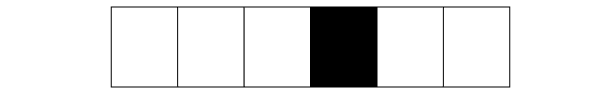
\includegraphics[width=0.4\textwidth]{rkplus_1.png}
    \centering
  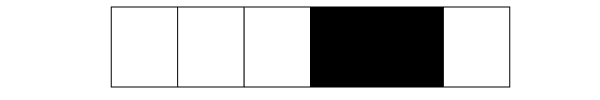
\includegraphics[width=0.4\textwidth]{rkplus_2.png}  
  \centering
  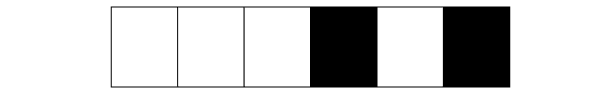
\includegraphics[width=0.4\textwidth]{rkplus_3.png}
    \centering
  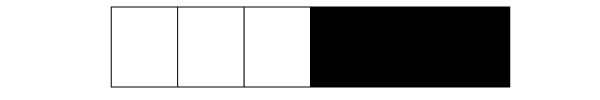
\includegraphics[width=0.4\textwidth]{rkplus_4.png}
  \caption{A robot located to the left of a 1D occupancy grid map $r_l$ composed of $n_{r,l}=6$ grid cells in $4$ cases. In each case, cells $1$--$3$ are free, cell $4$ is occupied, and cells $5$ and $6$ may or may not be occupied. All above outcomes correspond to the event $\mathbf{r}_{l,4+}$.}
  \label{fig:show_rkplus}
\end{figure}

\begin{prop}
For the $l$-th measurement ray, the a posteriori probability of the occupancy of the $k$-th cell, namely the ray inverse sensor model, is given by
\begin{align}
\label{eqn:RayISMAnswer}
P(\mathbf{r}_{l,k}|z_{t,l},X_{1:t},Z_{1:t-1})&=\eta_{t,l}\tilde P(\mathbf{r}_{l,k}|z_{t,l},X_{1:t},Z_{1:t-1}),
\end{align}
where the unnormalized probability of the inverse sensor model is defined as
\begin{align}
\label{eqn:Unnormalized}
& \tilde P(\mathbf{r}_{l,k}|z_{t,l},X_{1:t},Z_{1:t-1})%\nonumber\\&
=P(\mathbf{r}_{l,k}|X_{1:t-1},Z_{1:t-1})\nonumber\\
&\quad\times 
\bigg[\sum_{i=1}^{k-1}\bigg\{\prod_{j=0}^{i-1}P(\bar{\mathbf{r}}_{l,j}|X_{1:t-1},Z_{1:t-1})\bigg\}%\nonumber\\
%&\quad\times 
p(z_{t,l}|\mathbf{r}_{l,i+},X_t)P(\mathbf{r}_{l,i}|X_{1:t-1},Z_{1:t-1})\bigg]\nonumber\\
&\quad + \bigg\{\prod_{j=0}^{k-1}P(\bar{\mathbf{r}}_{l,j}|X_{1:t-1},Z_{1:t-1})\bigg\}%\nonumber\\
%&\quad\times 
p(z_{t,l}|\mathbf{r}_{l,k+},X_t)P(\mathbf{r}_{l,k}|X_{1:t-1},Z_{1:t-1}),
\end{align}
where $P(\bar{\mathbf{r}}_{l,0}|X_{1:t-1},Z_{1:t-1})=P(\mathbf{r}_{l,n_r+1}|X_{1:t-1},Z_{1:t-1})=1$ is chosen for convenience and $p(z_{t,l}|\mathbf{r}_{l,(n_r+1)+},X_t)$ represents the probability density of the measurement when all of cells in the field of view of the $l$-th ray is not occupied. The normalizer $\eta_{t,l}$ is given by
\begin{align}
\label{eqn:allEta}
\eta_{t,l}
&=
\bigg[\sum_{i=1}^{n_{r,l}+1}\bigg\{\prod_{j=0}^{i-1}P(\bar{\mathbf{r}}_{l,j}|X_{1:t-1},Z_{1:t-1})\bigg\}\nonumber\\&\quad\times p(z_{t,l}|\mathbf{r}_{l,i+},X_t)P(\mathbf{r}_{l,i}|X_{1:t-1},Z_{1:t-1})\bigg]^{-1},
\end{align}
and it is independent of the cell index $k$.
\end{prop}
\begin{proof}
See Appendix.
\end{proof}


%
%%respectively.
%These have the follow solutions that may be obtained in a computationally-efficient manner:
%\begin{align}
%\label{eqn:tildePresult}
%\tilde P(\mathbf{r}_k|z_{t,l},&X_{1:t},Z_{1:t-1})=P(\mathbf{r}_k|X_{1:t-1},Z_{1:t-1})\nonumber\\
%&\quad\times \sum_{i=1}^{k-1}\left\{\prod_{j=0}^{i-1}P(\bar{\mathbf{r}}_{l,j}|X_{1:t-1},Z_{1:t-1})\right\}\nonumber\\
%&\quad\times p(z_{t,l}|\mathbf{r}_{i+},X_t)P(\mathbf{r}_i|X_{1:t-1},Z_{1:t-1})
%\nonumber
%\\
%&\quad
%+
%\left\{\prod_{j=0}^{k-1}P(\bar{\mathbf{r}}_{l,j}|X_{1:t-1},Z_{1:t-1})\right\}\nonumber\\
%&\quad\times p(z_{t,l}|\mathbf{r}_{k+},X_t)P(\mathbf{r}_k|X_{1:t-1},Z_{1:t-1}),
%\\
%\label{eqn:tildePcomplementresult}
%\tilde P(\bar{\mathbf{r}}_k|z_{t,l},&X_{1:t},Z_{1:t-1})
%=P(\bar{\mathbf{r}}_k|X_{1:t-1},Z_{1:t-1})\nonumber\\
%&\quad\times \sum_{i=1}^{k-1}\left\{\prod_{j=0}^{i-1}P(\bar{\mathbf{r}}_{l,j}|X_{1:t-1},Z_{1:t-1})\right\}\nonumber\\
%&\quad\times p(z_{t,l}|\mathbf{r}_{i+},X_t)P(\mathbf{r}_i|X_{1:t-1},Z_{1:t-1})
%\nonumber
%\\
%&\quad
%+
%\sum_{i=k+1}^{n_r}\left\{\prod_{j=0}^{i-1}P(\bar{\mathbf{r}}_{l,j}|X_{1:t-1},Z_{1:t-1})\right\}\nonumber\\
%&\quad\times p(z_{t,l}|\mathbf{r}_{i+},X_t)P(\mathbf{r}_i|X_{1:t-1},Z_{1:t-1}).
%\end{align}


%
%
%Because $\mathbf{r}_k$ is binary, the following holds:
%\begin{align}
%\label{eqn:allEta}
%\eta_{t,l}&=\frac1{\tilde P(\mathbf{r}_k|z_{t,l},X_{1:t},Z_{1:t-1})+\tilde P(\bar{\mathbf{r}}_k|z_{t,l},X_{1:t},Z_{1:t-1})}\nonumber
%\\
%&=
%\bigg[\sum_{i=1}^{n_r}\left\{\prod_{j=0}^{i-1}P(\bar{\mathbf{r}}_{l,j}|X_{1:t-1},Z_{1:t-1})\right\}\nonumber\\&\quad\times p(z_{t,l}|\mathbf{r}_{i+},X_t)P(\mathbf{r}_i|X_{1:t-1},Z_{1:t-1})\bigg]^{-1},
%\end{align}
%where $\eta_{t,l}$ is independent of the index $k$ of the reduced map.
%Rearranging \refeqn{Unnormalized} and \refeqn{UnnormalizedCompl}, the ray inverse sensor model is 
%\begin{align}
%\label{eqn:RayISMAnswer}
%P(\mathbf{r}_k|z_{t,l},X_{1:t},Z_{1:t-1})&=\eta_{t,l}\tilde P(\mathbf{r}_k|z_{t,l},X_{1:t},Z_{1:t-1}),
%\\
%P(\bar{\mathbf{r}}_k|z_{t,l},X_{1:t},Z_{1:t-1})&=\eta_{t,l}\tilde P(\bar{\mathbf{r}}_k|z_{t,l},X_{1:t},Z_{1:t-1}),
%\end{align}
%respectively, where $\eta_{t,l}$ comes from \refeqn{allEta} and the unnormalized probabilities come from \refeqn{tildePresult} and \refeqn{tildePcomplementresult}.

Note that the a priori estimate, $P(\mathbf{r}_{l,k}|X_{1:t-1},Z_{1:t-1})$ and its compliment $\\P(\bar{\mathbf{r}}_{l,k}|X_{1:t-1},Z_{1:t-1})=1-P(\mathbf{r}_{l,k}|X_{1:t-1},Z_{1:t-1})$ are available at the $t$-th step. Then, \refeqn{RayISMAnswer} yields a sequential occupancy grid mapping that can be applied whenever new measurements are available. 

Compared with \refeqn{InvSenModWithProbDens}, where the terms of the summation should be repeated $2^{n_{r,l}}$ times \emph{per each cell of the reduced map}, the proposed expressions \refeqn{RayISMAnswer} and \refeqn{allEta} are \textit{substantially} simpler. In fact, if \refeqn{Unnormalized} and \refeqn{allEta} are obtained recursively, requiring the summation of $O(n_{r,l}+1)$ rather than $O(n_{r,l}\times2^{n_{r,l}})$ as previously thought for \emph{all cells of the reduced map}, this yields an algorithm that is $\mathbf{n_{r,l}\times2^{n_{r,l}}/(n_{r,l}+1)}$ \textbf{times faster}.


\paragraph{Scan Inverse Sensor Model}
The above one-dimensional ray inverse sensor model may be generalized into a two-dimensional scan inverse sensor model by updating the map sequentially for each ray, according to
%The most natural way to generalize the ray inverse sensor model into a scan inverse sensor model is applying the conditions in a recursive way,
\begin{align}
\label{eqn:RayByRayScanISM}
P&(\mathbf{m}_i|X_{1:t},Z_{1:t})%\nonumber\\&%=P(\mathbf{m}_i|X_{1:t},Z_{1:t-1}|z_{t,1},z_{t,2},\ldots,z_{t,n_z})\nonumber\\&
=P((\dots(((\mathbf{m}_i|X_{1:t},Z_{1:t-1})|z_{t,1})|z_{t,2})|\ldots)|z_{t,n_z}).
\end{align}
In short, this approach updates the map occupancies along the first measurement ray, then repeats this process for each subsequent ray until all rays composing the measurement scan have updated the map.

\subsection{Summary of Algorithm}\label{sec:SA}

In short, the proposed scan inverse sensor model is computed by \refeqn{RayISMAnswer}-\refeqn{RayByRayScanISM}. These are summarized in Algorithm \ref{alg:RayByRayISM} as a computationally efficient, recursive algorithm that avoids several repeated calculations of the same quantity. This algorithm utilizes temporary variables, where the required computational resources are minimized by computing the updated occupancy probabilities of all grid cells along a measurement ray together. Note that this function is only considering $l$-th ray at the $t$-th time step, where probabilities are subject to conditions on $X_{1:t},Z_{1:t-1},z_{t,1:l-1}$, so these are removed from the algorithm for simplicity.

%% More detailed (completed subscripts)
%\begin{table}[p]
%\begin{tabular}{ l }
%  Function: $P(\mathbf{r}_k|X_{1:t},Z_{1:t-1},z_{t,1:l})=\text{InverseSensorModel}(P(\mathbf{r}_k|X_{1:t},Z_{1:t-1},z_{t,1:l-1}),z_{t,l})$\\
%  for all $k\in\braces{1,2,\ldots,n_{r,l}}$\\
%  Note: all probabilities are conditioned on $X_{1:t},Z_{1:t-1},z_{t,1:l-1}$, so these are removed in probabilities.\\
%  Initialize $\eta^{-1}_{t,l}=0$ and $P(\bar{\mathbf{r}}_{0})=P(\bar{\mathbf{r}}_{n_{r,l}+1})=1$;\\
%  for all $k = 1,2,\ldots,n_{r,l}$\\
%   \ \ $P(\mathbf{r}_{k+}) = P(\bar{\mathbf{r}}_{0:k-1})P(\mathbf{r}_{k})$;\\
%   \ \ $P(\bar{\mathbf{r}}_{0:k})=P(\bar{\mathbf{r}}_{0:k-1})P(\bar{\mathbf{r}}_{k})$;\\
%   \ \ $a_\text{temp}=P(\mathbf{r}_{k+})p(z_l|\mathbf{r}_{k+},X_t)$;\\
%   \ \ $\tilde P(\mathbf{r}_{k}|z_{t,l})=P(\mathbf{r}_{k})\eta^{-1}_{t,l}+a_\text{temp}$;\\
%   \ \ $\eta^{-1}_{t,l}=\eta^{-1}_{t,l}+a_\text{temp}$;\\
%  end for\\
%  $\eta^{-1}_{t,l}=\eta^{-1}_{t,l}+P(\bar{\mathbf{r}}_{0:k})p(z_\text{max})$;\\
%  $P(\mathbf{r}_{k}|z_{t,l})=\eta_{t,l}\tilde P(\mathbf{r}_{k}|z_{t,l})$ for all $k\in\braces{1,2,\ldots,n_{r,l}}$;\\
%  \end{tabular}
%\caption{Inverse Sensor Model of an Individual Measurement Ray}
%\label{tab:RayByRayISM}
%\end{table}

% More simple (subscripts omitted)

\begin{algorithm}[H]
	Function: $P(\mathbf{r}_k|z)=\text{InverseSensorModel}(P(\mathbf{r}_k),z)$ $\forall$ $k\in\braces{1,2,\ldots,n_{r}}$\;
	Initialize $\eta^{-1}=0$ and $P(\bar{\mathbf{r}}_{0})=1$\;
	\For{$k=1,2,\ldots,n_{r}$}{
		$P(\mathbf{r}_{k+}) = P(\bar{\mathbf{r}}_{0:k-1})P(\mathbf{r}_{k})$\;
		$P(\bar{\mathbf{r}}_{0:k})=P(\bar{\mathbf{r}}_{0:k-1})(1-P(\mathbf{r}_{k}))$\;
    		$a_\text{temp}=P(\mathbf{r}_{k+})p(z_l|\mathbf{r}_{k+},X)$\;
   		$\tilde P(\mathbf{r}_{k}|z)=P(\mathbf{r}_{k})\eta^{-1}_{t,l}+a_\text{temp}$\;
   		$\eta^{-1}=\eta^{-1}+a_\text{temp}$\;
	}
	$\eta^{-1}=\eta^{-1}+P(\bar{\mathbf{r}}_{0:k})p(z_\text{max})$\;
	Return $P(\mathbf{r}_{k}|z)=\eta\tilde P(\mathbf{r}_{k}|z)$ for all $k\in\braces{1,2,\ldots,n_{r}}$\;
\caption{Inverse Sensor Model of an Individual Measurement Ray}
\label{alg:RayByRayISM}
\end{algorithm}



In contrast to the current approximate inverse sensor models, the proposed algorithm evaluates the exact inverse sensor model \refeqn{InvSenModWithProbDens} efficiently without relying on assumptions like \refeqn{AssumptionEarly}. Therefore, it yields substantially more accurate maps for the same set of measurements. These are illustrated by numerical examples and experiments in Sections \ref{sec:NumRes} and \ref{sec:ExpRes}.

This proposed mapping approach follows a Bayesian framework that focusses on occupied and free space, not tracking particular systems or mapping features, such as visual servoing~\cite{ChiDinChe14}. The proposed algorithm may be combined with feature-based approaches for object tracking or stabilization purposes, with the added challenge of associating occupied spaces with features.


\section{Computation of Expected Information Gain}
\label{sec:ExpectedInfoGain}

In this section, we present a method to determine the expected entropy from an individual measurement ray from a known pose. Based on this, an autonomous exploration algorithm will be developed in the next section.

%This method is based on the exact solution to occupancy grid mapping from~\cite{KauLeeAiMos16}.

\subsection{Single Ray Expected Value of Entropy}
Suppose there is a probabilistic map constructed by past measurements, namely \\$P(m|X_{1:t},Z_{1:t})$. We wish to compute the expected entropy when the next measurement is taken at the candidate pose $X_c=(x_c,R_c)$, consisting of location $x_c\in\Re^2$ and attitude $R_c\in\Sph^1$. Assume that the direction of the $l$-th ray is determined by the attitude $R_c$.
The expected entropy due to the $l$-th ray $z_{c,l}$ at position $x_c$ is
\begin{align}
\label{eqn:HRayInt}
\text{E}[H(P(m|&X_{1:t},Z_{1:t},x_c,z_{c,l}))]
\nonumber\\&
=\int_{z_\text{min}}^{z_\text{max}}
H(P(m|X_{1:t},Z_{1:t},x_c,z_{c,l}))%\nonumber\\&\qquad\times 
p(z_{c,l}|X_{1:t},Z_{1:t},x_c)
dz_{c,l}.
\end{align}
%where $z_\text{min}$ and $z_\text{max}$ are sensor limits. Considering the continuous space of possible measurements of $z_{c,l}$ would make \refeqn{HRayInt} intractable to calculate. Thus, w
We discretize the measurement ray space such that $z_{c,l}$ falls on points along the measurement ray intersecting with grid cell edges. %, similar with how occupancy grid mapping decomposes continuous space into grid cells of length $\alpha$.
The discretized expected value of \refeqn{HRayInt} is
\begin{align}
\label{eqn:DiscExpEntropyRay}
\text{E}[H(P(&m|X_{1:t},Z_{1:t},x_c,z_{c,l}))]
\nonumber\\&=\sum_{k=1}^{n_{r,l}+1}\bigg\{H(P(m|X_{1:t},Z_{1:t},x_c,z_{c,l,k}))%\nonumber\\&\qquad\times 
P(z_{c,l,k}|X_{1:t},Z_{1:t},x_c)\bigg\},
\end{align}
where index $z_{c,l,k}$ is the distance from position $x_c$ to the $k$-th grid cell of the $l$-th reduced map $r_l$, known from geometry.

Standing alone, the term $P(z_{c,l,k}|X_{1:t},Z_{1:t},x_c)$ from \refeqn{DiscExpEntropyRay} has a convoluted meaning because the depth $z_{c,l,k}$ does not directly depend on the map. However, we present a method to obtain this discretized probability. %Despite how this term is replaced with a normalizer in ~\cite{ThrBurFox05} replaces
Following the assumption that $z_{c,l}$ is discretized to known distances, the probabilities are proportional to their densities, as the area under the density curve is infinitesimal and fixed. Accounting for all cases, the probability is
\begin{align}
\label{eqn:ProbWithDelta}
P(z_{c,l,k}|X_{1:t},Z_{1:t},x_c)=\frac{p(z_{c,l,k}|X_{1:t},Z_{1:t},x_c)}{\sum_{i=1}^{n_{r,l}+1}p(z_{c,l,i}|X_{1:t},Z_{1:t},x_c)}.
\end{align}
Conveniently, this density corresponds to the inverse normalizer according to \refeqn{BayesRuleRayISM},
\begin{align}
\label{eqn:DiscretizedProb}
p(z_{c,l,k}|X_{1:t},X_c,Z_{1:t})=\eta_{c,l,k}^{-1},
\end{align}
where $\eta_{c,l,k}^{-1}$ is defined in \refeqn{allEta}. %However, instead of evaluating the $t$-th pose $X_t$ and measured ray $z_{t,l}$, we simply consider $X_c$ and ray depth $z_{c,l,k}$ based on histories $X_{1:t}$ and $Z_{1:t}$ to obtain the inverse normalizer,
Updating variable subscripts, the normalizer becomes
\begin{align}
\label{eqn:allEtaAtC}
\eta_{c,l,k}^{-1}
&=
\sum_{i=1}^{n_{r,l}+1}\bigg\{\prod_{j=0}^{i-1}P(\bar{\mathbf{r}}_{l,j}|X_{1:t},Z_{1:t})\bigg\}%\nonumber\\&\qquad\times 
p(z_{c,l,k}|\mathbf{r}_{l,i+},X_c)P(\mathbf{r}_{l,i}|X_{1:t},Z_{1:t}).
\end{align}
By substituting \refeqn{ProbWithDelta} and \refeqn{DiscretizedProb} into \refeqn{DiscExpEntropyRay}, the expected entropy at $X_c$ from individual measurement ray $z_{c,l}$ is
\begin{align}
\label{eqn:HRayComplete}
\text{E}[H(P&(m|X_{1:t},Z_{1:t},x_c,z_{c,l}))]\nonumber\\&=
\left(\sum_{i=1}^{n_{r,l}+1}\eta_{c,l,i}^{-1}\right)^{-1}%\nonumber\\&\quad\quad\times
\sum_{k=1}^{n_{r,l}+1}\bigg\{H(P(m|X_{1:t},Z_{1:t},x_c,z_{c,l,k}))\eta_{c,l,k}^{-1}\bigg\},
\end{align}
where $\eta_{c,l,k}^{-1}$ is taken from \refeqn{allEtaAtC}.
Here, \refeqn{HRayComplete} provides the expected entropies for those cells inside the field of view of $r_l$. %; cells outside this reduced map are trivially changed by $0$ due to $z_{c,l}$.
The entropies of cells outside the field of view remain unchanged.


\subsection{Approximation of Expected Ray Entropy}

The order of computation for each measurement ray is $\mathcal O((n_{r,l}+1)^2)$ since the summations of \refeqn{allEtaAtC} are embedded in \refeqn{HRayComplete}. However, several of those intersections provide negligible information since the probability of the $l$-th measurement ray capturing certain cell depths is close to zero.

The approximation of expected ray entropy provides a method to reduce the computation of \refeqn{allEtaAtC} substantially. This goal is achieved by systematically selecting a smaller set of grid cells to consider over the summations of \refeqn{allEtaAtC} and \refeqn{HRayComplete}.
The smaller set is determined by the probability that each cell is captured by the measurement ray, known as the detection probability. This can be found recursively as
\begin{align}
\label{eqn:ProbOfFirstCell}
&P(\mathbf{r}_{l,k+}|X_{1:t},Z_{1:t})%\nonumber\\&
=\bigg\{\prod_{j=0}^{k-1}P(\bar{\mathbf{r}}_{l,j}|X_{1:t},Z_{1:t})\bigg\}P(\mathbf{r}_{l,k}|X_{1:t},Z_{1:t}),
\end{align}
which is the probability that $\mathbf{r}_{l,k}$ is the closest occupied grid cell based on past poses and measurement scans, independent of cells beyond the $k$-th cell from $x_c$.
Let $\hat n>0$ be a fixed number of grid cells for all rays such that $\hat n\leq n_{r,l}+1$ for all $l$.
Let $\hat{r}_{l}$ correspond to the grid cells that yield the $\hat{n}$ maximum values of \refeqn{ProbOfFirstCell} (the $\hat n$ most likely ray detections), indexed by increasing distance from candidate location $x_c$.
By replacing the reduced map $r_l$ with $\hat{r}_l$ and changing the summation limits to $\braces{1,2,...,\hat n}$ in \refeqn{allEtaAtC} and \refeqn{HRayComplete}, the order of computation is reduced to $\mathcal O({\hat{n}}^2)$.
Even though the value of $n_{r,l}$ is different among various rays in general, $\hat n$ is fixed, so the computational order is fixed as well.
In short, this method reduces the required computation substantially by systematically neglecting those grid cells with little effect. It can be noted that if $\hat n=n_{r,l}+1$, the ray objective function is computed without approximation.


\subsection{1D Ray Expected Information Gain Algorithm}

We present an algorithm pseudocode providing the necessary steps to obtain the objective function for a single measurement ray (Algorithm \ref{alg:RayExpectedEntropyGain}). Much like the algorithm pseudocode for the inverse sensor model (Algorithm \ref{alg:RayByRayISM}), the variable $a_\text{temp}$ serves as an intermediate variable designed to avoid repeated calculations.
Since this algorithm operates as a function, fixed indices and condition variables are removed for simplification. 



\begin{algorithm}[H]
	Function: $\mathcal I_\text{ray}=\text{RayExpInfoGain}(x,P(r),z_{1:n_{r}})$\;
	Initialize $P(\bar{\mathbf{r}}_{0})=P(\hat{\bar{\mathbf{r}}}_{0})=P(\bar{\mathbf{r}}_{n_{r}+1})=1$\;
	\For{$k = 1,2,\ldots,n_{r}+1$}{
		$P(\mathbf{r}_{k+}) = P(\bar{\mathbf{r}}_{0:k-1})P(\mathbf{r}_{k})$\;
		$P(\bar{\mathbf{r}}_{0:k})=P(\bar{\mathbf{r}}_{0:k-1})(1-P(\mathbf{r}_{k}))$\;
	}
	Find $\hat r\subset r$ of the $\hat n$ greatest values of 
	$\braces{P(\mathbf{r}_{1+}),P(\mathbf{r}_{2+}),\ldots,P(\mathbf{r}_{(n_{r}+1)+})}$\;
	\For{$k = 1,2,\ldots,\hat{n}$}{
		$P(\hat{\mathbf{r}}_{k+}) = P(\hat{\bar{\mathbf{r}}}_{0:k-1})P(\hat{\mathbf{r}}_{k})$\;
		$P(\hat{\bar{\mathbf{r}}}_{0:k})=P(\hat{\bar{\mathbf{r}}}_{0:k-1})P(\hat{\bar{\mathbf{r}}}_{k})$\;
	}
	\For{$k_\text{m}=1,2,\ldots,\hat n$}{
		Initialize $\eta^{-1}_{k_\text{m}}=0$\;
		\For{$k_\text{c}=1,2,\ldots,\hat n$}{
			$a_\text{temp}=P(\hat{\mathbf{r}}_{k_\text{c}+})p(z_{k_\text{m}}|\hat{\mathbf{r}}_{k_\text{c}+},x)$\;
			$\tilde P(\hat{\mathbf{r}}_{k_\text{c}}|x,z_{k_\text{m}})=P(\hat{\mathbf{r}}_{k_\text{c}})\eta^{-1}_{k_\text{m}}+a_\text{temp}$\;
			$\eta^{-1}_{k_\text{m}}=\eta^{-1}_{k_\text{m}}+a_\text{temp}$\;
		}
		$P(\hat{\mathbf{r}}_{k_\text{c}}|x,z_{k_\text{m}})=\eta_{k_\text{m}}\tilde P(\hat{\mathbf{r}}_{k_\text{c}}|x,z_{k_\text{m}})$ for all $k_\text{c}=1,2,\ldots,\hat n$\;
	}
	$P(z_{k_\text{m}}|x)=\frac{\eta^{-1}_{k_\text{m}}}{\sum_{i=1}^{\hat n}\eta^{-1}_{i}}$ for $k_\text{m}=1,2,\ldots,\hat n$\;
	Initialize $\mathcal I_\text{ray}=0$\;
	\For{$k_\text{c}=1,2,\ldots,\hat n$}{
		$\mathcal I_\text{ray}=\mathcal I_\text{ray}+H(P(\hat{\mathbf{r}}_{k_\text{c}}))$\;
		\For{$k_\text{m}=1,2,\ldots,\hat n$}{
			$\mathcal I_\text{ray} = \mathcal I_\text{ray}-H(P(\hat{\mathbf{r}}_{k_\text{c}}|x_c,z_{k_\text{m}}))P(z_{k_\text{m}}|x_{c})$\;
		}
	}
	Return: $\mathcal I_\text{ray}$\\
\caption{Expected Information Gain from a Measurement Ray}
\label{alg:RayExpectedEntropyGain}
\end{algorithm}



\subsection{Numerical Justification for Approximation}

The purpose of this numerical example is to provide evidence that the approximations are reasonable and increase the algorithm speed substantially.
Since a measurement ray produces a depth measurement in a single direction, we only consider a 1D map where the grid cells have spacing $\alpha=0.2$ meters, and the properties of the range sensor are based on the Microsoft Kinect~\cite{PirRutBisSch11,KhoElb12} with maximum reading depth $z_\text{max}=4$m ($20$ grid cells inside the sensor FOV). The goal is to compare the expected entropy $\text{E}[H(P(m|X_{1:t},Z_{1:t},x_c,z_{c,l}))]$ from \refeqn{HRayComplete} and with an approximation $\text{E}[H_\text{approx}(P(m|X_{1:t},Z_{1:t},x_c,z_{c,l}))]$, which only considers $\hat n$ grid cells with highest detection probability \refeqn{ProbOfFirstCell}.

We consider $100$ probabilistic maps to obtain Monte Carlo results to evaluate the approximate entropy. In every Monte Carlo trial, each grid cell has an $80\%$ chance of being free and a $20\%$ chance of receiving an a priori probability uniformly distributed between $0$ and $1$. 
%We consider $100$ probabilistic maps to obtain Monte Carlo results to evaluate the approximate entropy. In every Monte Carlo trial, each grid cell has an $80\%$ chance of being free, and the remaining $20\%$ of grid cells are given an a priori probability uniformly distributed between $0$ and $1$. 
Several metrics serve to evaluate $\text{E}[H(P(m|X_{1:t},Z_{1:t},x_c,z_{c,l}))]$ with $\text{E}[H_\text{approx}(P(m|X_{1:t},Z_{1:t},x_c,z_{c,l}))]$. The median expected entropy change is $\text{E}[H(P(m|X_{1:t},Z_{1:t},x_c,z_{c,l}))]-H(P(m|X_{1:t},Z_{1:t}))=-0.83792$. The error for the $100$ Monte Carlo cases is defined simply as
\begin{align}
e_{H}&=\frac1{100}\sum_{i=1}^{100}\text{abs}\bigg(\text{E}[H(P(m|X_{1:t},Z_{1:t},x_c,z_{c,l}))]\nonumber\\&\qquad\quad-\text{E}[H_\text{approx}(P(m|X_{1:t},Z_{1:t},x_c,z_{c,l}))]\bigg).
\end{align}
The Monte Carlo trials are repeated for $\hat n=\braces{1,2,\ldots,10}$ and the results are plotted in Figure \ref{fig:ApproxJust}.
This example shows a typical case when the summation limits generated from \refeqn{ProbOfFirstCell} have only small effects on \refeqn{HRayComplete}, while providing very large improvements in reducing computation.

\begin{figure}
	\centering
    	\begin{subfigure}[b]{0.35\textwidth}
        		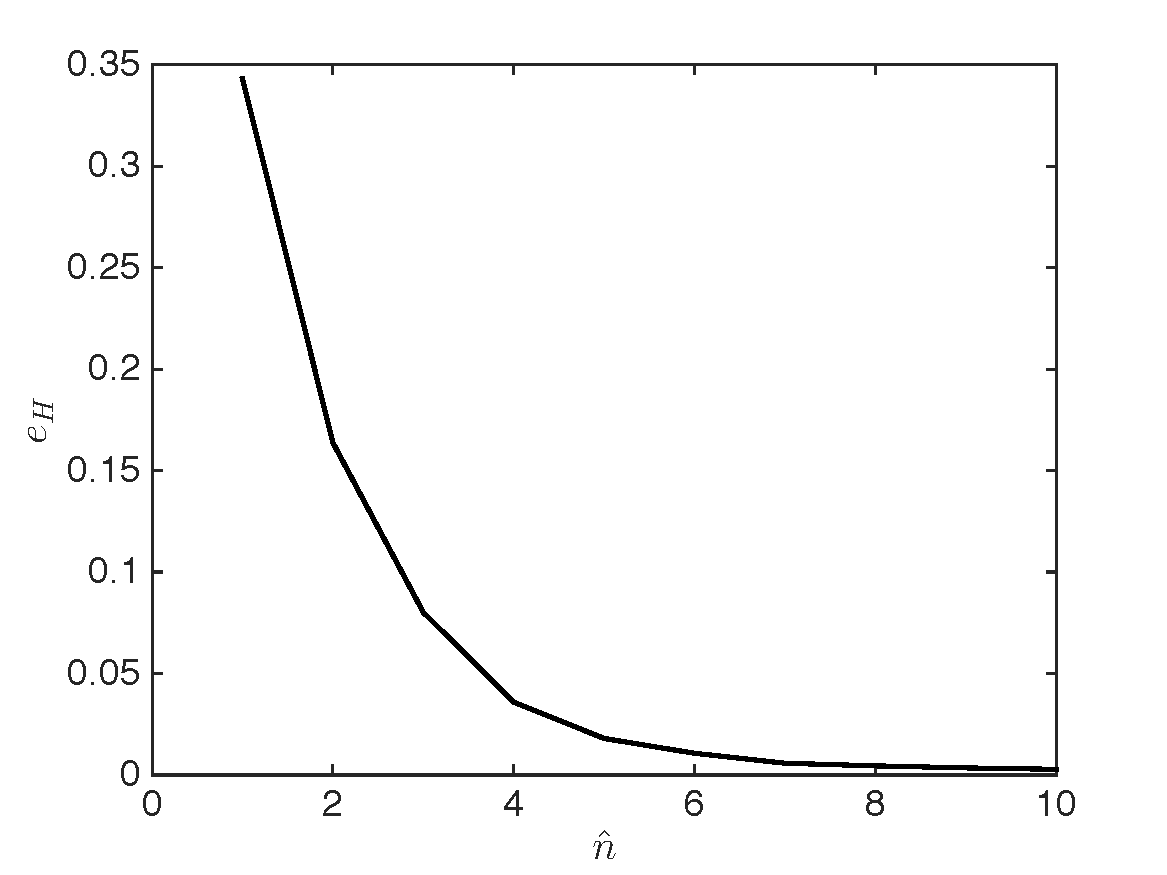
\includegraphics[width=\textwidth]{JustifyApprox_eH.pdf}
        		\caption{Entropy Error}
        		\label{fig:H_err}
    	\end{subfigure}
%	\hspace*{0.1\columnwidth}
	\begin{subfigure}[b]{0.35\textwidth}
        		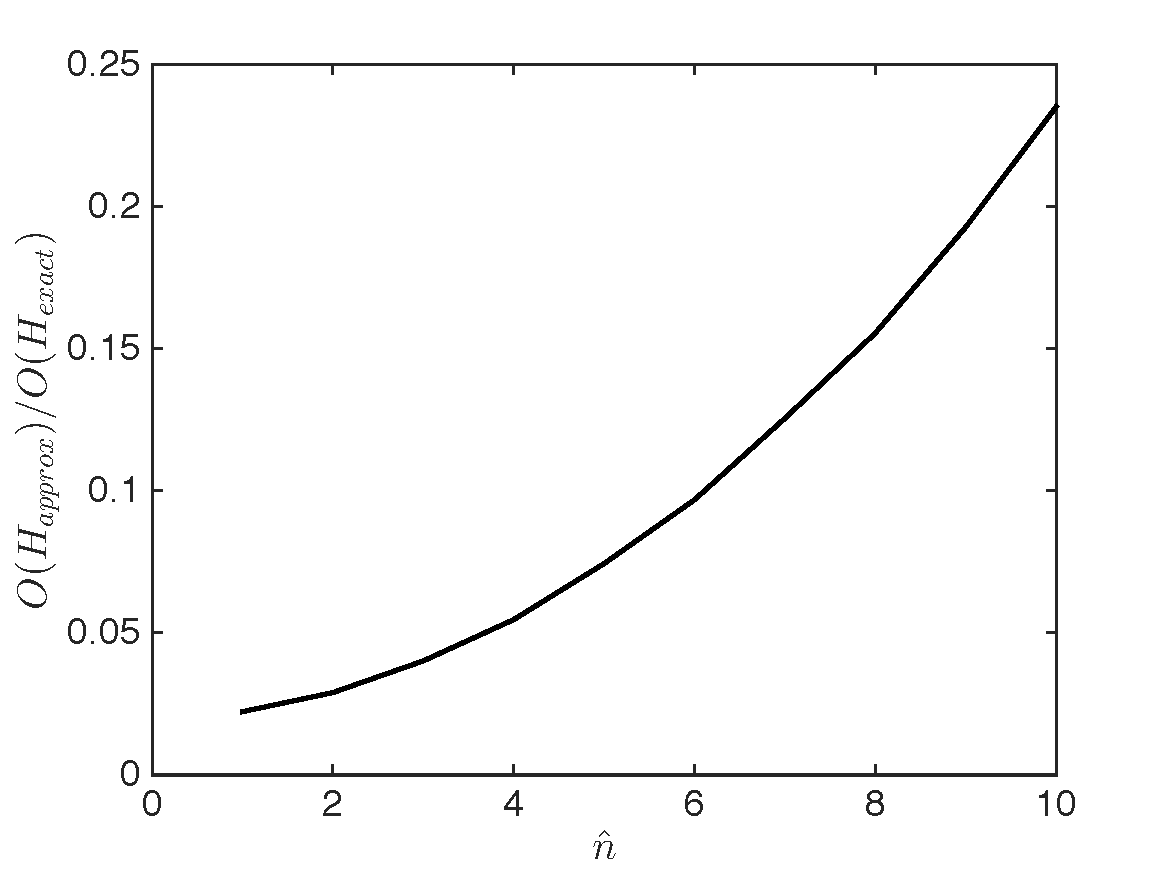
\includegraphics[width=\textwidth]{JustifyApprox_t.pdf}
        		\caption{Computation Ratio}
        		\label{fig:H_comp_ratio}
    	\end{subfigure}
%	\begin{subfigure}[Computation Ratio]
%		{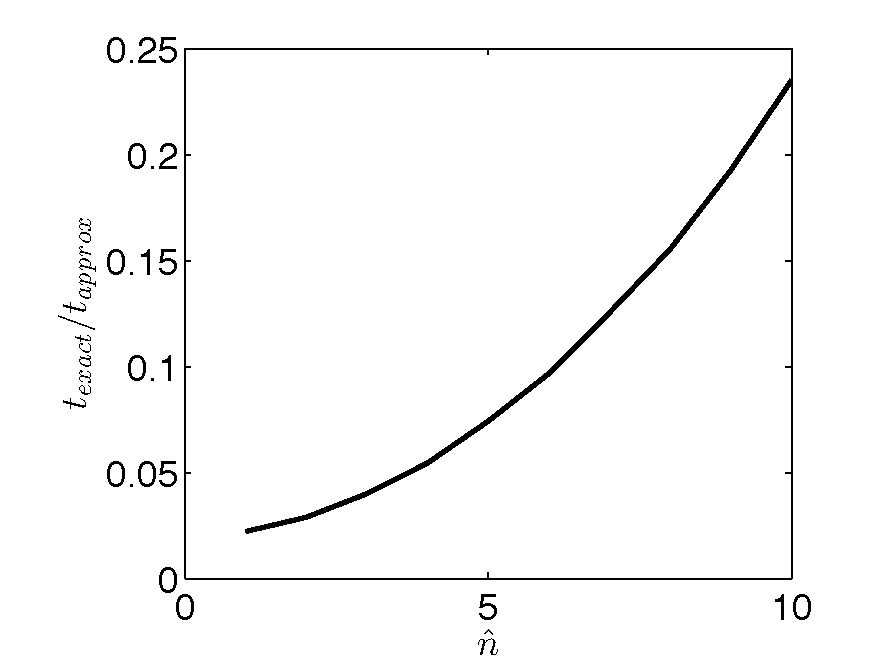
\includegraphics[height=0.35\columnwidth]{JustifyApprox_tRatio.pdf}
%	}
%	\end{subfigure}

\caption{The entropy error is decreased at the cost of increasing computation time in this Monte Carlo 1D measurement ray expected entropy case.}
\label{fig:ApproxJust}
\end{figure}












\section{Autonomous Exploration}

In this section, we develop an autonomous exploration scheme inside a 2D environment based on choosing movements that minimize map entropy and avoid collisions.

\subsection{Pose Selection Optimization}

The objective is to choose a future pose that minimizes the map uncertainty, such that the robot can autonomously move toward this optimal goal. The robot pose is selected among various positions and attitudes. Since searching over all locations and attitudes would require infinite computational resources, these search spaces are discretized into a limited number of robot attitudes and positions.
The procedure involves three steps. First, the attitude that maximizes the information gain objective function is selected at each candidate future pose location. Second, the location with the maximum objective function of all candidates is selected. Thus, the optimal attitude and the optimal location compose the optimal future pose. Finally, the robot determines and follows a collision-free path to the optimal future pose. This process is repeated, resulting in autonomous exploration.

%First, the optimal attitude for an arbitrary location is presented. Then, two methods to select pose candidates, namely \emph{expanding ring} and \emph{complete Cartesian}, are described below, with a brief discussion of the benefits and drawbacks of choosing each search space. Finally, the equations and conditions to determine an optimal future pose are presented.

\paragraph{Attitude Optimization}
Consider a collision-free pose candidate at an arbitrary location $x_c$. At this pose, consider $n_d$ evenly-spaced measurement rays oriented radially outward from the robot in a circular pattern (see red lines in Figure \ref{fig:OptProcess}). These rays are denoted $\braces{z_{c,1},z_{c,2},\ldots,z_{c,n_d}}$. Attitudes correspond to the rays such that the robot sensor is aligned with the ray direction, and these are denoted $\braces{R_{c,1},R_{c,2},\ldots,R_{c,n_d}}$, where the scan with attitude $R_{c,d}$ might cover several ray directions depending on the sensor field of view (FOV). We choose optimal attitude $R_c^*$ as the summation of the expected entropy changes covered by the scan,
\begin{align}
\label{eqn:FindRc}
&R_c^*=\argmax_{R_{c,d}}\sum_{z_{c,i}\in R_{c,d}\text{ FOV}}\bigg(H(P(m|X_{1:t},Z_{1:t}))\nonumber\\&\qquad\quad\quad\quad\quad
-\text{E}[H(P(m|X_{1:t},Z_{1:t},x_c,z_{c,i}))]\bigg).
%\mathcal I_\text{ray}(x_c,z_{c,i})\right).
\end{align}

This method provides the attitude that maximizes the information gain at an arbitrary location in 2D space. The set of candidate positions that warrant consideration is determined with one of two methods, namely \emph{expanding ring} and \emph{complete Cartesian}, described next.

\paragraph{Expanding Ring}
The expanding ring technique is advantageous for searching local solutions quickly, only considering distant future poses when necessary. The key idea is that future candidate locations lie on a circular ``ring'' centered around the robot, evenly spaced around the ring (see red circles in Figure \ref{fig:OptProcess}), and the ring is expanded if certain criteria are not met. More explicitly, consider $n_c$ candidate locations denoted by $x_c\in\braces{x_1,x_2,\ldots,x_{n_c}}$ located with the distance $\delta$ away from the robot. Any location that violates inequality constraint \refeqn{CollisionInequalityConstraint} is excluded to avoid collisions. The set of optimal attitudes at each candidate location is $\braces{R^*_{1},R^*_{2},\ldots,R^*_{n_c}}$, obtained from \refeqn{FindRc}. The objective function \refeqn{ObjFun} is computed by a summation about the $n_d$ rays as %\refeqn{Objective},
\begin{align}
\label{eqn:ObjFunApprox}
\mathcal I(x_c,R_c^*)&\approx \sum_{z_{c,i}\in R_{c}^*\text{ FOV}}\bigg(H(P(m|X_{1:t},Z_{1:t}))\nonumber\\&\qquad-\text{E}\left[H(P(m|X_{1:t},Z_{1:t},x_c,R_c^*,z_{c,i}))\right]\bigg),
\\
x_c^*&=\argmax_{x_c}\mathcal I(x_c,R_c^*).
\end{align}
At the optimal pose $X^*_c=(x^*_c,R^*_c)$, the resulting information gain must satisfy $\mathcal I(X_c^*)\geq\mathcal I_\text{min}$, where $\mathcal I_\text{min}$ is some minimum threshold for expected information gain; robot motion is only justified when the expected information gain is significantly large. If the minimum threshold is not met, the ring of candidate pose locations is increased such that $n_c$ and $\delta$ are multiplied by a scale function $\lambda>1$.
This process is repeated until the expected information gain of the optimal pose is at least $\mathcal I_\text{min}$, or all candidates lie in collision zones or outside map limits. %A pseudocode of the process is found in Table \ref{tab:Alg_AutomousExploration}.

The primary advantage of the expanding ring approach to search the 2D space is that the number of pose candidates need not be proportional to the map area, and that local maxima tend to fall within short distances of the current robot pose. The main drawback is that poses outside a small local region of the robot are frequently neglected, and the robot frequently executes repeated short motions, often without large information gains.

\paragraph{Complete Cartesian}
The complete Cartesian method to search the 2D space provides candidates located fixed distance $d$ apart in each Cartesian direction. This approach is advantageous for capturing expected information gains in regions outside of the immediate vicinity of the robot, but must be applied carefully to avoid issues with computational bottlenecks due to the potentially-large search space.

Similar to the expanding ring approach, $n_c$ candidate pose locations are considered, where those violating \refeqn{CollisionInequalityConstraint} are neglected from further consideration. However, unlike the ring expanding approach, the candidates have different distances from the robot in general, so the objective function is modified to enforce a cost on the squared distance from the current pose location $x_t$ to the candidate location $x_c$, i.e.,
\begin{align}
\label{eqn:ObjFunApproxCompleteCartesian}
\mathcal I&(x_c,R_c^*,x_t)\approx \sum_{z_{c,i}\in R_{c}^*\text{ FOV}}\bigg(H(P(m|X_{1:t},Z_{1:t}))\nonumber\\&-\text{E}\left[H(P(m|X_{1:t},Z_{1:t},x_c,R_c^*(x_c),z_{c,i}))\right]\bigg)-k_\text{dist}(x_t-x_c)^\T(x_t-x_c),
\end{align}
where weighting function $k_\text{dist}$ represents the sensitivity to avoiding large motions across the map. Furthermore, the same candidate locations are considered throughout the repeated processes of exploration, and the map cell occupancies are assumed static. Therefore, if candidate location $x_c$ fails to satisfy $\mathcal I(x_c,R_c^*,x_t)\geq\mathcal I_\text{min}$, then $x_c$ need \emph{never} be considered again. Avoiding these unnecessary calculations yields a greatly lowered computational burden, particularly late in exploration where several regions are collision-free but disadvantageous to revisit.


\begin{figure}
\vspace*{0.1\columnwidth}
\centerline{
	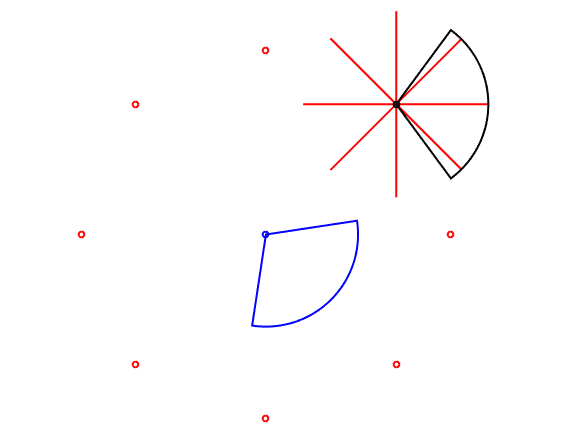
\includegraphics[height=0.35\columnwidth]{ExampleOptimalPose.png}
}
\begin{picture}(0,0)(0,0)
\setlength{\unitlength}{0.1\columnwidth}\scriptsize
\put(4.4,2.1){\color{blue}$X_t$}
\put(5.9,1.9){\color{red}$x_1$}
\put(2.9,2.0){\color{red}$x_5$}
\put(4.4,3.6){\color{red}$x_3$}
\put(4.4,0.6){\color{red}$x_7$}
\put(5.4,3.0){\color{red}$x_2$}
\put(3.3,3.1){\color{red}$x_4$}
\put(3.3,1.0){\color{red}$x_6$}
\put(5.4,1.0){\color{red}$x_8$}
\put(6.8,3.1){\color{red}$z_{2,1}$}
\put(4.5,3.1){\color{red}$z_{2,5}$}
\put(5.6,4.1){\color{red}$z_{2,3}$}
\put(5.6,2.2){\color{red}$z_{2,7}$}
\put(6.5,3.7){\color{red}$z_{2,2}$}
\put(4.9,3.8){\color{red}$z_{2,4}$}
\put(5.0,2.5){\color{red}$z_{2,6}$}
\put(6.5,2.5){\color{red}$z_{2,8}$}
\put(6.1,2.9){$X_c^*$}
\end{picture}
\caption{This figure illustrates the expanding ring method. Initially, a robot (blue circle) views down and left (blue sector). Then, the robot considers $n_c=8$ poses (red circles) as possible candidates for where to move next. For each candidate, $n_d=8$ directions are considered (red lines, only displayed on candidate location $c=2$). Then, the expected entropy of each ray is calculated. The scan (red sector) covering those rays with the largest expected entropy decreases is chosen for each candidate, and the best candidate $X_c^*$ (black circle: location, black sector: scan) is chosen to maximize information gain. Finally, Dijkstra's algorithm provides the collision-free motion between $X_t$ and $X_c^*$, and the process is repeated.
}
\label{fig:OptProcess}
\end{figure}

%avoiding collisions subject to the inequality constraint \refeqn{CollisionInequalityConstraint}. 

\paragraph{Motion Planning}
Once the optimal future pose $X_c^*$ is selected, the robot must traverse its environment to reach $X_c^*$ without collisions.
The locations of cells on a grid-based map provide nodes for Dijkstra's algorithm~\cite{Dij59},~\cite{Dij11}. At each node, \refeqn{CollisionInequalityConstraint} must be satisfied for the node to be considered reachable, and edges between nodes correspond to neighboring grid cells.
Dijkstra's algorithm provides a relatively simple motion planning strategy to move from $x_t$ to $x_c^*$ that avoids collisions and local minima. 

The trajectory to follow the path outlined by Dijkstra's algorithm is determined with a linear constrained least squares optimization, assuming the robot follows a polynomial trajectory with fixed speed. The starting and ending positions and attitudes may be constrained, and polynomials patched together for long trajectories share a common position and velocity with respect to time. Then, the robot tracks this trajectory until the robot falls within acceptable thresholds of the final optimal pose. For generality of the proposed exploration algorithm, any position controller yielding robotic motion that follows this desired trajectory may be selected. Once the robot completes this motion, the entire process is repeated.
%The complete autonomous exploration process is summarized in Table \ref{tab:Alg_AutomousExploration}.


%The first pseudocode in table \ref{tab:Alg_AutomousExploration} outlines how a candidate pose is selected given an objective function. The second pseudocode in table \ref{tab:Alg_ObjFun}

%\begin{table}[p]
%\begin{tabular}{ l }
%%  Define $n_c$: number of candidate locations\\
%%  Define $n_d$: number of evenly-spaced measurement rays per candidate\\
%  Given: $t=1$, $X_{1}$, $Z_{1}$, $P(m|X_{1},Z_{1})$ from the inverse sensor model\\
%  TrajectoryComplete = false;\\
%  while TrajectoryComplete = false\\
%  \ \ if $X_{t+1}$ is unknown\\
%  \ \ \ \ MotionPlanning = false;\\
%  \ \ \ \ while MotionPlanning = false\\
%  \ \ \ \ \ \ for $c = 1,2,\ldots,n_c$\\
%  \ \ \ \ \ \ \ \ Candidate location: $x_{c}$ from evenly-spaced circle around\\
%  \ \ \ \ \ \ \ \ $X_t$ with radius $\delta$;\\
%  \ \ \ \ \ \ \ \ for $d=1,2,\ldots,n_d$\\
%  \ \ \ \ \ \ \ \ \ \ Obtain reduced map $r_{c,d}$ with $n_{r_{c,d}}$ intersections\\
%  \ \ \ \ \ \ \ \ \ \ through grid cells with depths $z_{c,d,1:n_{r,d}}$ from geometry;\\
%  \ \ \ \ \ \ \ \ \ \ $\mathcal I_\text{ray}(x_c,z_{c,d})=\text{RayExpInfoGain}(x_c,P(r_{c,d}),z_{c,d,1:n_{r,d}})$;\\
%  \ \ \ \ \ \ \ \ end for\\
%  \ \ \ \ \ \ \ \ $R_{c}^*=\argmax_{R_c}\left(\sum_{z_{c,i}\in R_c \text{ FOV}}\mathcal I_\text{ray}(x_c,z_{c,i})\right)$;\\%\argmax_{R}{\sum_{d=1}^{n_d}\mathcal I_{\text{ray},c,d}|d\in\text{FOV}(R))}$;\\
%  \ \ \ \ \ \ \ \ $\mathcal I(x_c,R_c^*)=\sum_{z_{c,i}\in R_c^* \text{ FOV}}\mathcal I_\text{ray}(x_c,z_{c,i})$;\\%\sum_{d\in \text{FOV}(R_c^*)}\mathcal I_{\text{ray}_{c,d}}$;\\
%  \ \ \ \ \ \ end for\\
%  \ \ \ \ \ \ $x_c^*=\argmax_{x_c}\mathcal I(x_c,R_c^*)$;\\
%  \ \ \ \ \ \ $X_c^*=\braces{x_c^*,R_c^*}$;\\
%  \ \ \ \ \ \ if $\mathcal I(X_c^*)<\mathcal I_\text{min}$\\
%  \ \ \ \ \ \ \ \ $n_c=\text{round}(\lambda n_c)$;\\
%  \ \ \ \ \ \ \ \ $\delta=\lambda \delta$;\\
%  \ \ \ \ \ \ else\\
%  \ \ \ \ \ \ \ \ Obtain $X_{t+1},X_{t+2},\ldots,X_{c}^*$ using Dijkstra's algorithm and minimum rotation;\\
%  \ \ \ \ \ \ \ \ Reset $n_c$ and $\delta$ to initial values;\\
%  \ \ \ \ \ \ \ \ MotionPlanning = true;\\  
%  \ \ \ \ \ \ end if\\
%  \ \ \ \ end while\\
%%  $X_c^*=\argmax_{X}$\mathcal I_{\text{ray},c
%%  \ \ $\mathcal D\subset\braces{1,2,\ldots,n_d}$ represents scan coverage of candidate rays\\
%%  \ \ The $c$-th pose candidate: $X_{c}=\braces{x_{c},R_{c}}$;\\
%%   end for\\
%%  $X_c^*=\argmin_{X_c}({\Delta H(X_c)}|X_c\in\braces{X_1,X_2,\ldots,X_{n_c}})$;\\
%%  Motion planner generates a collision-free path between $X_t$ to $X_c^*$\\
%%  Move to $X_{t+1}$, obtain $Z_{t+1}$, and find $P(m|X_{1:t+1},Z_{1:t+1})$;
%  \ \ end if\\
%  \ \ t = t+1;\\
%  \ \ Obtain $P(m|X_{1:t},Z_{1:t})$ from the inverse sensor model;\\
%  \ \ if map $m$ is completely explored\\
%  \ \ \ \ TrajectoryComplete = true;\\
%  \ \ end if\\
%  end while
%
%
%\end{tabular}
%\caption{Autonomous Exploration via Expected Information Gain from Expanding Ring Searches}
%\label{tab:Alg_AutomousExploration}
%\end{table}










\section{Numerical Examples}
\label{sec:NumRes}

The efficacy of the proposed algorithms are verified by numerical examples. First, the occupancy grid mapping strategies are simulated in Section \ref{sec:NEOGC}, followed by numerical examples for autonomous exploration in Section \ref{sec:NEAE}. 

% It is common practice to approximate\refeqn{InvSenModWithProbDens} with a simplified function, frequently following the structure of the approximate inverse sensor model proposed in~\cite{And09}. The main idea of this approach is that the probability of a cell being occupied ($i$) near a measurement is high (measurement likely hits this cell), ($ii$) between the robot and the measurement is low (measurement passes through this cell), and ($iii$) beyond the measurement is unchanged (the robot cannot measure through a wall/object). The function is based on intuition, not thorough mathematical derivation. In short, this approach simplifies the inverse sensor model at the cost of accuracy.

%The Kinect depth sensor is used as an example, with specifications from~\cite{KhoElb12}. With these parameters and the identical set of measurements, the exact solution is compared with a benchmark algorithm for a Kinect sensor taken from summarized as follows.




\subsection{Occupancy Grid Mapping}\label{sec:NEOGC}

First, we compare the proposed exact solution to the inverse sensor model summarized in Algorithm \ref{alg:RayByRayISM} with an approximate algorithm presented in~\cite{PirRutBisSch11,KhoElb12}, summarized as follows. The probability that the $i$-th grid cell $\mathbf{m}_i$ is occupied conditioned on the measurement ray $z_{t,l}$ at the pose $X_t$ is the continuous function
\begin{align*}
%\label{eqn:ISM_Approx_1}
&P(\mathbf{m}_i|z_{t,l},X_t)%\nonumber\\&
=\begin{cases}
0.3+(\frac{k}{\sigma\sqrt{2\pi}}+0.2)e^{-\frac12\left(\frac{\hat z_{l,i}-z_{t,l}}{\sigma}\right)^2}\ &\text{if}\ \hat z_{l,i} \leq z_{t,l},%z_{t,l}\leq \hat z_{l,i},
\\
0.5+\frac{k}{\sigma\sqrt{2\pi}}e^{-\frac12\left(\frac{\hat z_{l,i}-z_{t,l}}{\sigma}\right)^2}\ &\text{otherwise},
\end{cases}
\end{align*}
which is based on the expected distance to the cell $\hat z_{l,i}$ with parameters $k=\sigma=0.6$. This follows the structure of the approximate inverse sensor model proposed in~\cite{And09}. The main idea of this approach is that the probability of a cell being occupied (i) near a measurement is high (measurement likely hits this cell), (ii) between the robot and the measurement is low (measurement passes through this cell), and (iii) beyond the measurement is unchanged (the robot cannot measure through a wall/object). 
Then, these probabilities are combined in a weighted fashion such that all measurements rays of scan $Z_t$ simultaneously update the same grid cell in a log-odds format,
\begin{align*}
%\label{eqn:ISM_Approx_2}
&\log\left(\frac{P(\mathbf{m}_i|Z_{t},X_t)}{1-P(\mathbf{m}_i|Z_{t},X_t)}\right)
%\nonumber\\&
=
\frac1{\sum_{z_{t,l}\in\mathbf{m}_i}\hat z_{l,i}}\sum_{z_{t,l}\in\mathbf{m}_i}\log\left(\frac{P(\mathbf{m}_i|z_{t,l},X_t)}{1-P(\mathbf{m}_i|z_{t,l},X_t)}\hat z_{l,i}\right).
\end{align*}

%Given the same poses and measurement sets, the proposed algorithm from \refeqn{RayISMAnswer}-\refeqn{RayByRayScanISM} are compared with the approximate algorithm described above. A probabilistic map consisting of NUMX by NUMY square grid cells with edge length ALPHA is assumed to accurately represent the occupancy of the environment surrounding a robot. The robot follows (SOMETHING ABOUT THE TRAJECTORY). With both algorithms, the probabilistic maps are updated in real time.
%
%(PARAGRAPH ABOUT MAP CLARITY, ENTROPY, AND COMPUATION TIME)

Table~\ref{tab:penn} shows the mapping parameters and data specifications for the actual odometry and lidar measurements from University of Pennsylvania through Coursera open course~\cite{coursera}. Among these parameters, cell resolution and the number of rays have the greatest impact on computation. In general, the finer the grid, the greater the memory and computational requirements are because the computational order of \refeqn{RayISMAnswer} grows linearly with the number of grid cells inside the sensor range limits. Since the inverse sensor models are combined sequentially as shown in \refeqn{RayByRayScanISM}, the number of rays considered are proportional to the computation order as well.
Figure~\ref{fig:penn_map} shows the direct comparison of the resulting map based on the approximate and proposed inverse sensor model.
As shown in the figure, both approaches capture the structure of the environment. However, the significant differences can be seen in the certain area of the map such as in Figure~\ref{fig:penn_map_zoom}.
The differences can be clearly depicted in Figure~\ref{fig:entropy_comp} where entropy of maps are compared at frame 2280.
The red part of the map shows the maximum  entropy whereas blue shows lowest entropy for the cell.
Finally, overall improvement was demonstrated in Figure~\ref{fig:entropy} resulting improved entropy value per grid cell throughout the mapping process.
In short, the proposed exact occupancy grid mapping produced a cleaner map with lower entropy from the same set of measurements.

\begin{center}
\captionof{table}{Experimental parameters provided from dataset}
\label{tab:penn}
    \begin{tabular}{r | c}
        Parameters & Value\\ \hline\hline
        Map dimension & 576x448 [pixel]\\
        Resolution & 1/16 [m]\\
        Scan angle & [-2.36, 2.36]\\
        Ray number & 1081\\
        Total frame & Every 120 scans out of 3701\\
    \end{tabular}
\end{center}

\begin{figure}[!ht]
    \centering
    \begin{subfigure}[t]{0.8\columnwidth}
        \centering
        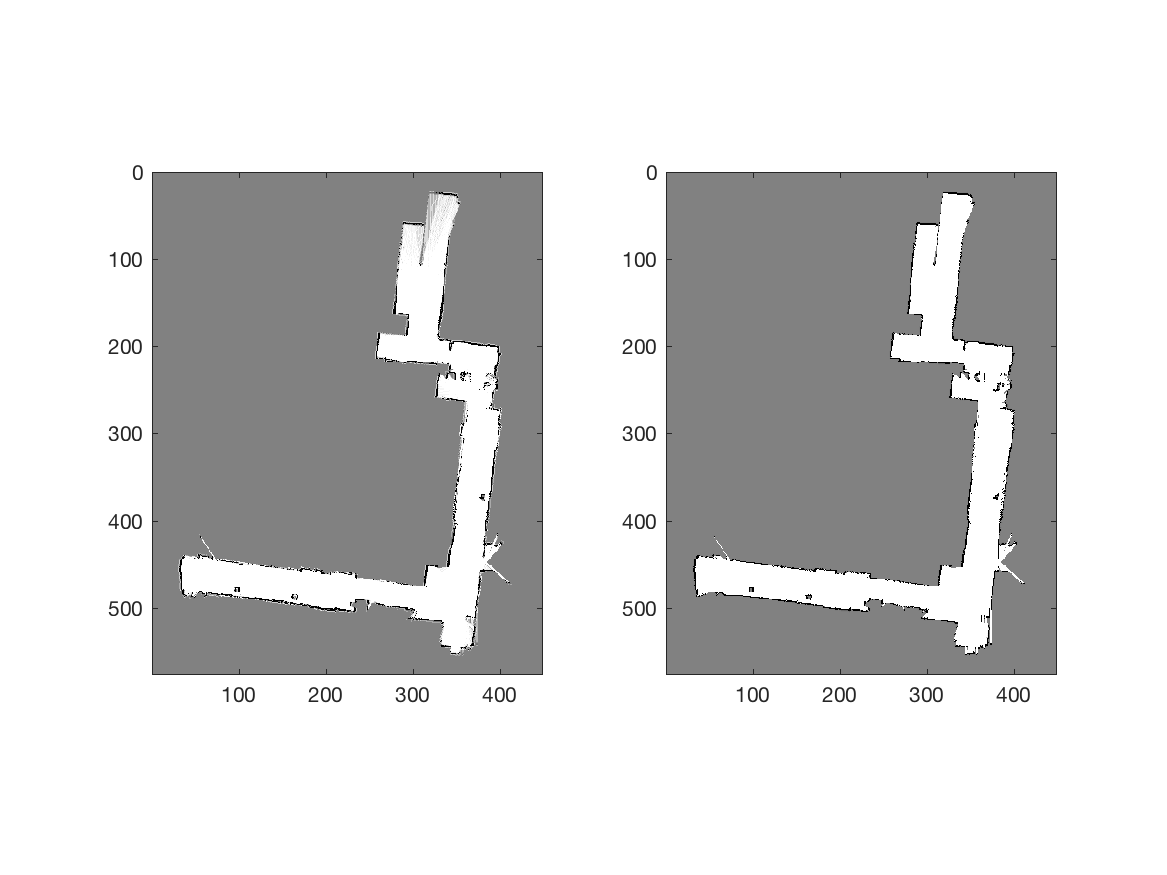
\includegraphics[trim={1.5cm 3.5cm 1.5cm 1.5cm},clip,width=\textwidth]{map_comparison.png}
        \caption{Comparison of the total mapped environment based on the approximate (left) and proposed (right) inverse sensor model.}
        \label{fig:penn_map_total}
    \end{subfigure}
    \begin{subfigure}[t]{0.8\columnwidth}
        \centering
        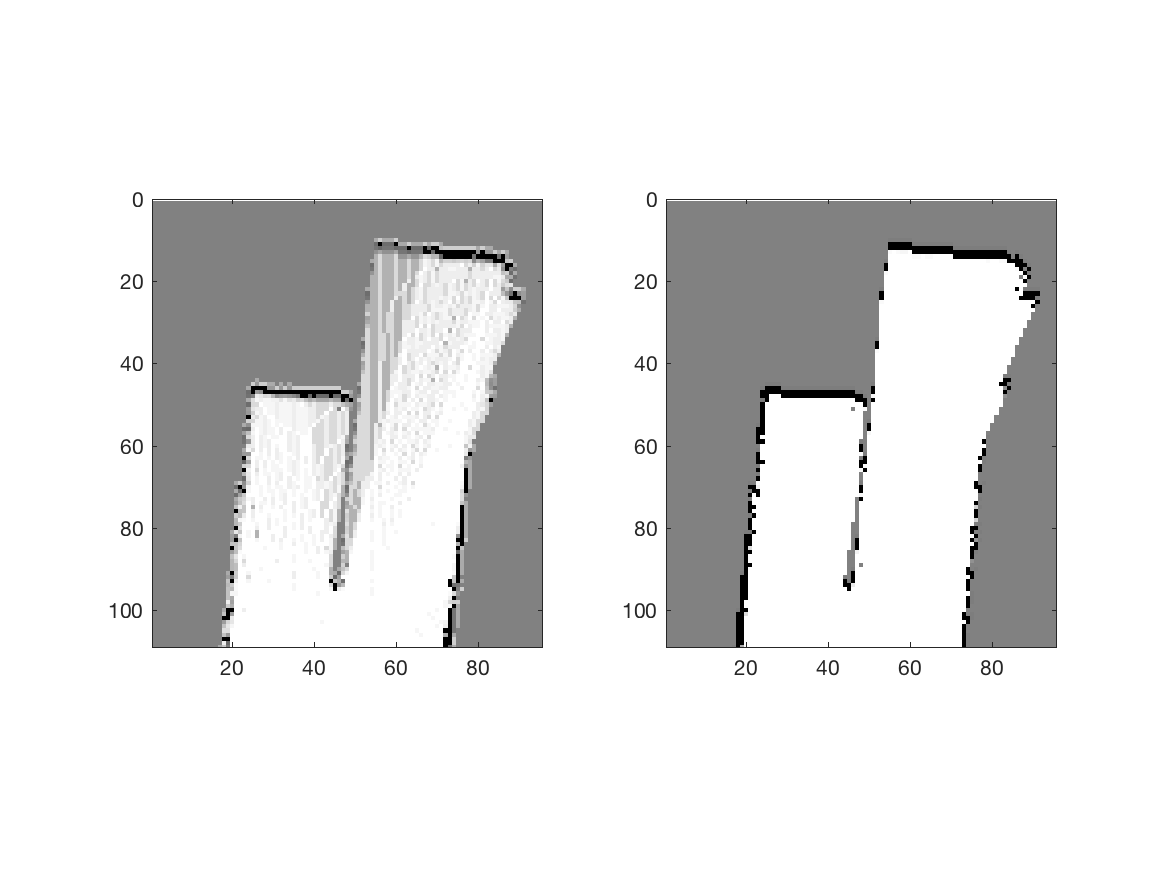
\includegraphics[trim={1.5cm 3.5cm 1.5cm 1.5cm},clip,width=\textwidth]{map_zoom.png}
        \caption{Evidence of significant improvement at certain area of the map.}
        \label{fig:penn_map_zoom}
    \end{subfigure}
    \caption{Using experimental sensor data, the map was generated using an approximate and the proposed exact inverse sensor models. The laser sensor and odometry data used for the experiment was provided by University of Pennsylvania open course robotics estimation and learning on Coursera~\cite{coursera}.}
    \label{fig:penn_map}
\end{figure}


\begin{figure}[!ht]
    \centering
    \begin{subfigure}[t]{0.35\columnwidth}
        \centering
        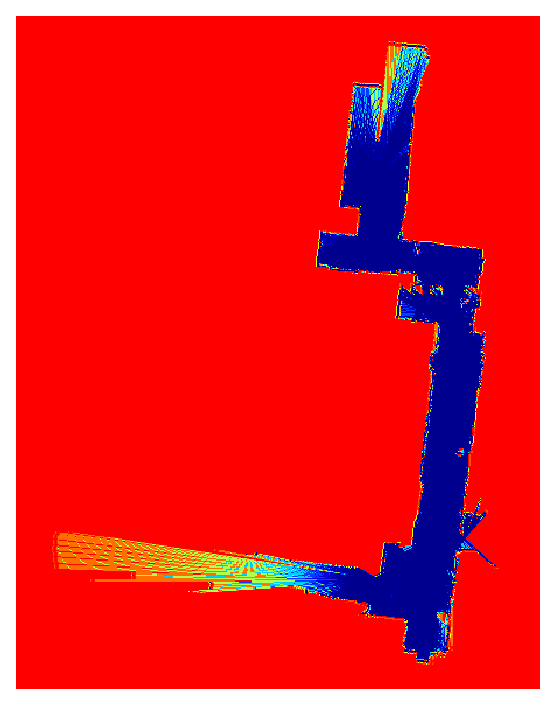
\includegraphics[width=\textwidth]{AISM_Image_inf_19.pdf}
        \caption{Approximate inverse sensor model}
        \label{fig:AISM}
    \end{subfigure}
    \begin{subfigure}[t]{0.35\columnwidth}
        \centering
        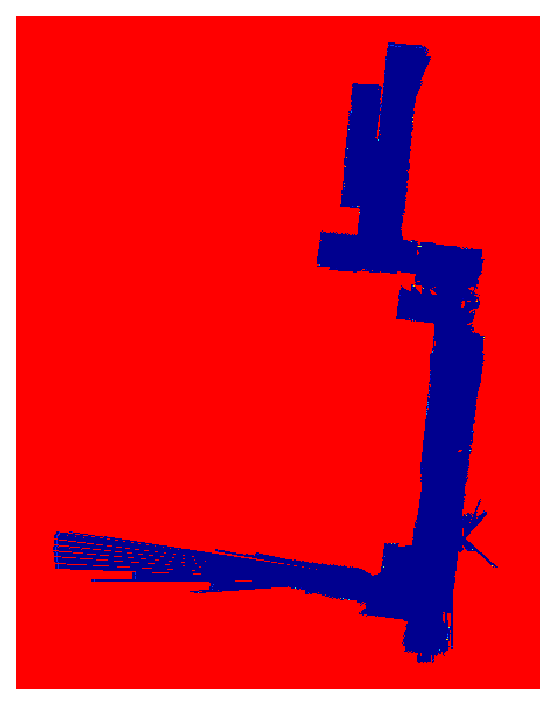
\includegraphics[width=\textwidth]{EISM_Image_inf_19.pdf}
        \caption{Exact inverse sensor model}
        \label{fig:EISM}
    \end{subfigure}
    \caption{The entropy is compared between the approximate and proposed exact inverse sensor models at step 2280. The blue areas show the lowest entropy while red shows highest.}
    \label{fig:entropy_comp}
\end{figure}


\begin{figure}
  \centering
  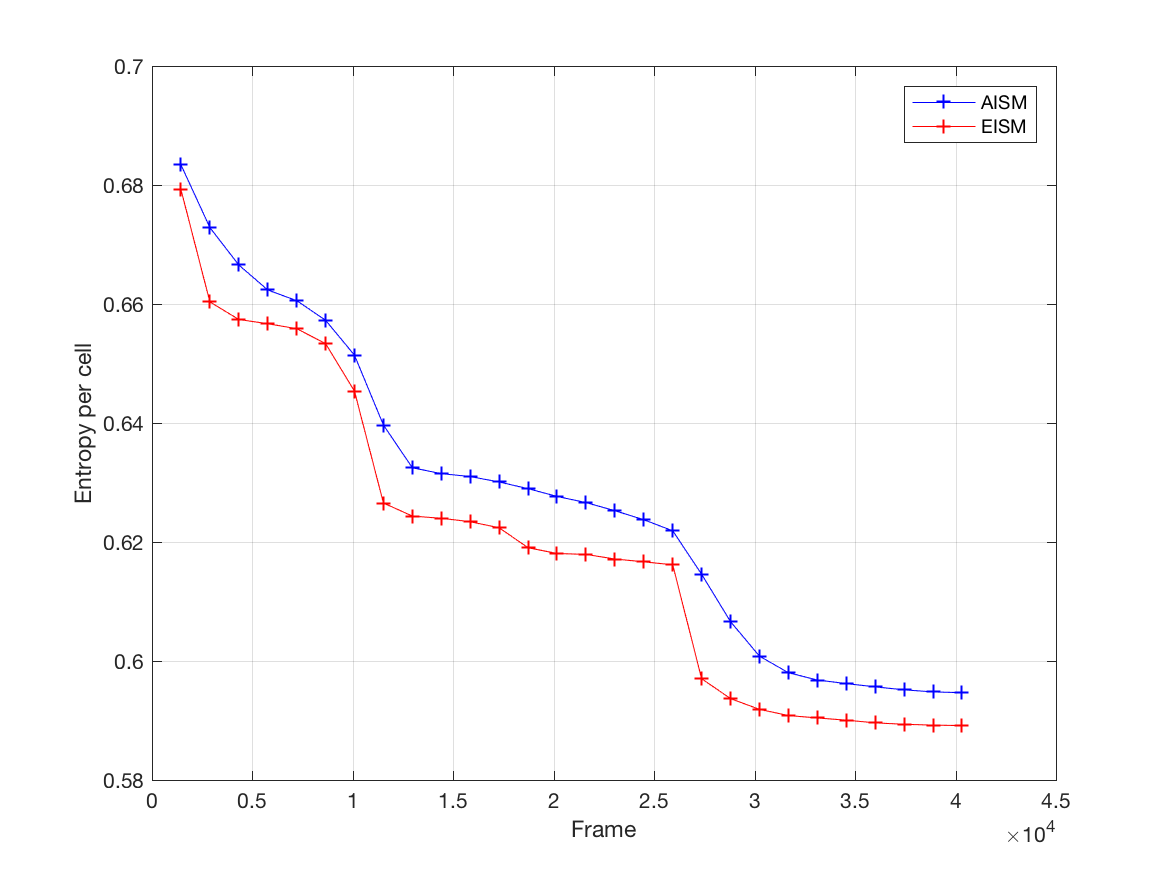
\includegraphics[width=0.7\textwidth]{entropy_frame.png}
  \caption{The map entropies of the approximate inverse sensor model (blue) and the proposed exact inverse sensor model (red) show that the exact version yields a more certain occupancy grid map.}
  \label{fig:entropy}
\end{figure}




%\paragraph{Computation Time}
%The proposed ray inverse sensor model is designed to maintain the accuracy of the exact solution with substantial computational improvements.
%A $1$-dimensional example is simulated on a Mac desktop computer with $11$ grid cells, $10$ of which are visible to the robot, where the same depth measurement is used for all occupancy grid algorithms.
%The computational time of the exact solution is computed in the conventional manner according to \refeqn{InvSenModWithProbDens} in $2.3314$ seconds to obtain the same solution of \refeqn{RayISMAnswer} from \refeqn{Unnormalized} and \refeqn{allEta} in just $0.0027$ seconds, which is $874.77$ times faster.
%The approximate ray inverse sensor model completes in $0.0011$ seconds, but this algorithm does not follow a forward sensor model, so the probabilities of the map may be inaccurate.








%\subsection{Trajectory Map Building}
%In this numerical example, we consider a robot in a two-dimensional environment composed of ten wall edges, and the robot follows a figure-eight curve, then turns around and completes the same curve in the reverse direction.
%The map is composed of $100\times100$ square grid cells with edge length of $1$ cm.
%A forward sensor model $p(z_t|m,X_t)$~\cite{ThrBurFox05} is constructed according to the specifications of the Kinect sensor~\cite{KhoElb12}, and a pseudo-random measurement scan is sampled at each time step via the inverse transform sampling~\cite{DevBK86}. The same set of measurements updated each second are used with both occupancy grid mapping algorithms to construct the map.
%
%The resulting maps are illustrated in Figure \ref{fig:NumResOccProbs} for both algorithms, where it is shown that the proposed algorithm yields a substantially more accurate and clear map with less uncertainty. To quantify the degree of map uncertainty, we define the entropy of the map as 
%\begin{align*}
%&H(P(m|X_{1:t},Z_{1:t}))=\nonumber\\
%&-\sum_{i=1}^n\big\{P(\mathbf{m}_i|X_{1:t},Z_{1:t})\log P(\mathbf{m}_i|X_{1:t},Z_{1:t})\nonumber\\
%&+(1-P(\mathbf{m}_i|X_{1:t},Z_{1:t}))\log(1-P(\mathbf{m}_i|X_{1:t},Z_{1:t}))\big\},
%\end{align*}
%which is maximized when the probability of occupancy is $0.5$ for all cells (more uncertain), and it is minimized when they are either $0$ or $1$ (less uncertain). 
%
%The change of the map entropy over time, and the entropy of the completed maps, for both methods are depicted in Figure \ref{fig:NumResOccH}. The subfigure (a) illustrates that the proposed exact inverse sensor model exhibits rapid decreases of entropies, and smaller entropies always. The resulting terminal map obtained from the proposed approach, shown in the subfigure (b), has less uncertainty than (c) constructed by the approximate model. In short, the proposed approach is more efficient at extracting information about the environment from the same set of set measurements. 


\subsection{Autonomous Exploration}\label{sec:NEAE}

%Maximizing the proposed expected information gain serves as the objective for autonomous exploration. A robot begins in a completely uncertain environment, except for the grid cells inside the immediate vicinity the robot location. 

%At each time step, the robot receives a measurement scan, where the probabilistic properties of the sensor are taken from~\cite{PirRutBisSch11,KhoElb12}. Then, the $n_c=8$ evenly-spaced candidate locations about a circle of radius $\delta=0.5$m around the current pose location are considered, where $n_d=16$ measurement rays are evenly-spaced about the candidate location.  When no current candidates yield expected information gains above $\mathcal I_\text{min}=1.25$, $\lambda=1.25$ is multiplied to the current $n_c$ and $\delta$ values. The motion of the robot is restricted to movement on grid cells satisfying \refeqn{CollisionInequalityConstraint} with $\beta=0.01$. Dijkstra's algorithm guides the robot through the environment without collision. 

Next, the proposed exploration approach is applied to the floor plan of Intel Research Lab, illustrated in Figure~\ref{fig:intel}.
The robot explores its surroundings with an occupancy grid with $90,000$ cells where grid cell edges are $\alpha=0.1$m, composing a map with dimensions $30\text{m}\times30\text{m}$.
The initial probability $P(\mathbf{m}_i)=1\times10^{-10}\approx0$ (minimum value for free space) for grid cells covered by the circular robot of radius $0.3$m and $P(\mathbf{m}_i)=0.5$ for all other cells.
For added safety, cells falling within $0.6$m of the robot are considered inside the possible collision zone $\mathcal{C}_X$, from \refeqn{CollisionInequalityConstraint}, where $\beta=0.1$ is selected. 
% One practical implication of \refeqn{CollisionInequalityConstraint} is that cells with greater occupancy probabilities inside $\mathcal{C}_X$ tend to fall near the perimeter of the region because internal cells are typically well-known to be free assuming the robot covered open space beforehand. Thus, a fairly large $\beta=0.1$ selected.

The robot follows the complete Cartesian candidate search method to determine future poses, with $k_\text{dist}=5$ to avoid large motions with little added expected information gains. Due to the large size of the map, candidates below the expected information gain of $1.25$ are neglected from future consideration.

The time sequence of the exploration for every 5~minutes are simulated in ROS Stage 2D environment. The corresponding simulation results are illustrated in Figure \ref{fig:IRL} and a video is available at \href{https://www.youtube.com/watch?v=5VdzKHreB_s}{\WriteBlue{https://www.youtube.com/watch?v=5VdzKHreB\_s}}.
Lighter red dots and darker blue dots in the explored area correlate to the level of information gain at those positions with low and high value, respectively. It is shown that the proposed autonomous exploration algorithm successfully mapped the complicated environment composed of a number of rooms, narrow hallways, and open spaces that are irregularly shaped.


%This approach not only achieved exploration of the entire environment but also improved computational efficiency.


\begin{figure}
    \centering
    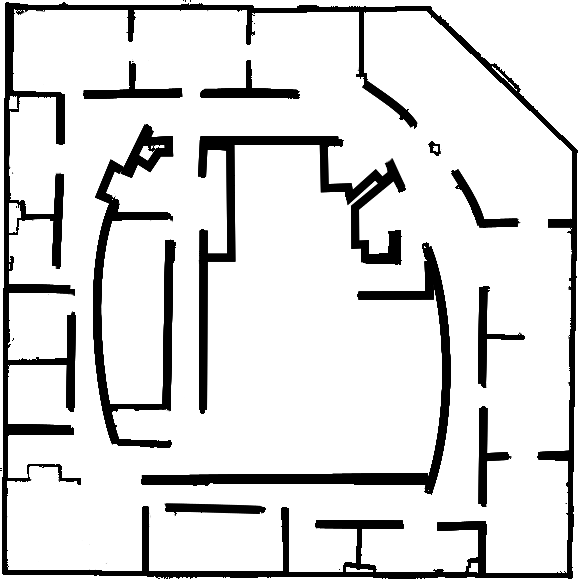
\includegraphics[width=0.4\textwidth]{intel_clean.png}
    \caption{Modified Intel Research Lab floor plan form the SLAM benchmark~\cite{kummerle2009measuring}.}
\label{fig:intel}
\end{figure}


\begin{figure}[!ht]
    \centering
    \begin{subfigure}[t]{0.3\columnwidth}
        \centering
        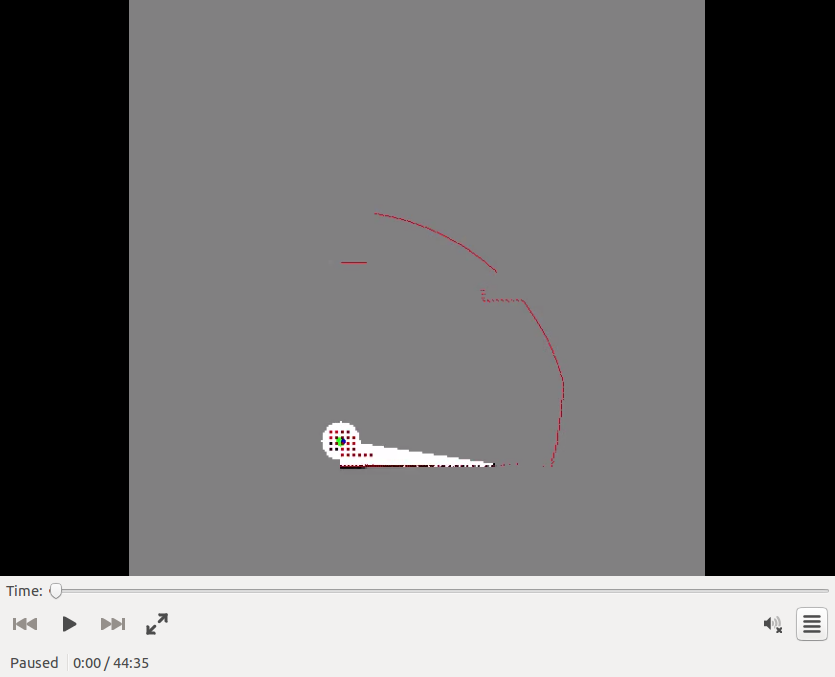
\includegraphics[trim = {4.6cm 3.8cm 4.6cm 0}, clip, width=\textwidth]{0min.png}
        \caption{$t=0$ min}
        \label{fig:IRL0min}
    \end{subfigure}
    \begin{subfigure}[t]{0.3\columnwidth}
        \centering
        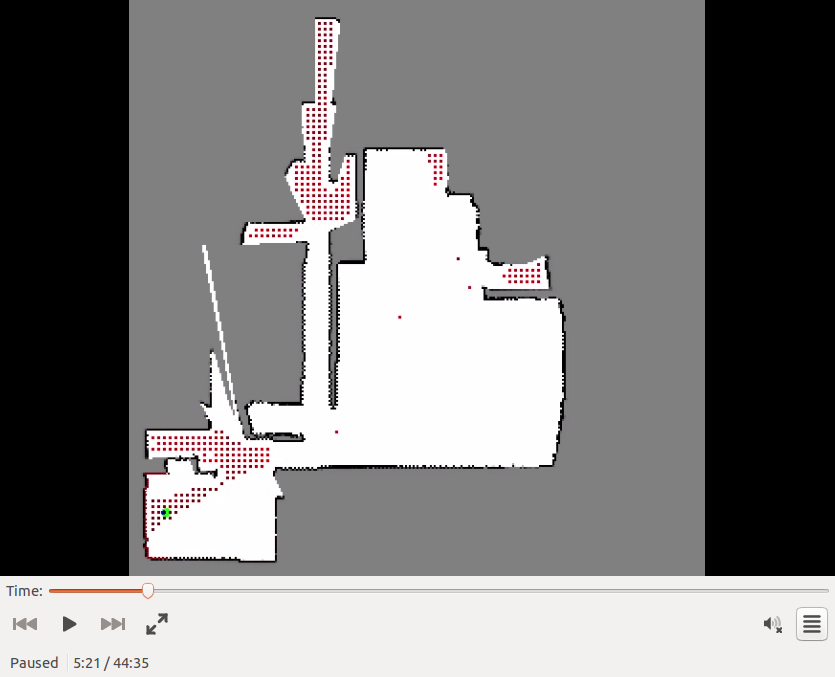
\includegraphics[trim = {4.6cm 3.8cm 4.6cm 0}, clip, width=\textwidth]{5min.png}
        \caption{$t=5$ min}
        \label{fig:IRL5min}
    \end{subfigure}
    \begin{subfigure}[t]{0.3\columnwidth}
           \centering
           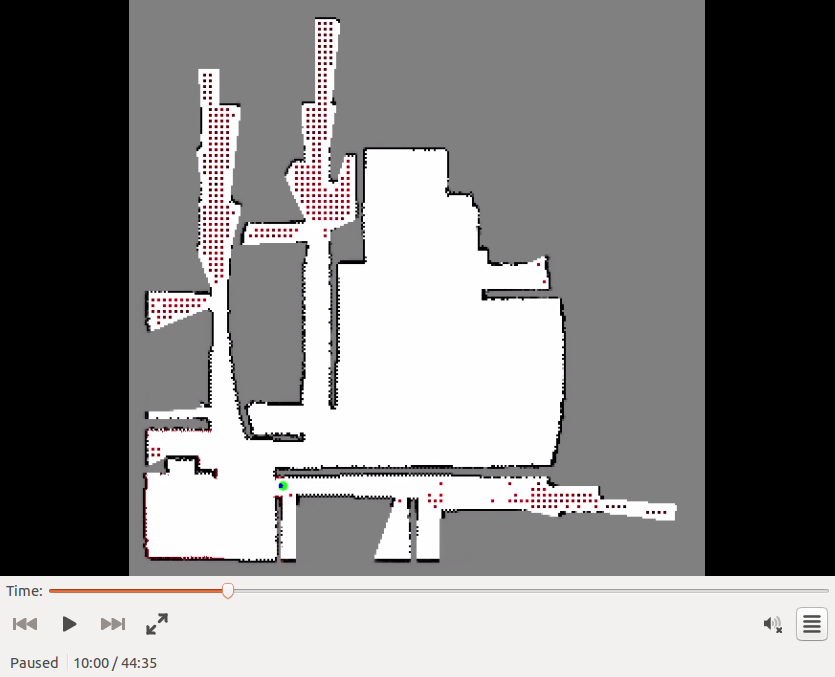
\includegraphics[trim = {4.6cm 3.8cm 4.6cm 0}, clip, width=\textwidth]{10min.png}
        \caption{$t=10$ min}
        \label{fig:IRL10min}
    \end{subfigure}
    \begin{subfigure}[t]{0.3\columnwidth}
           \centering
           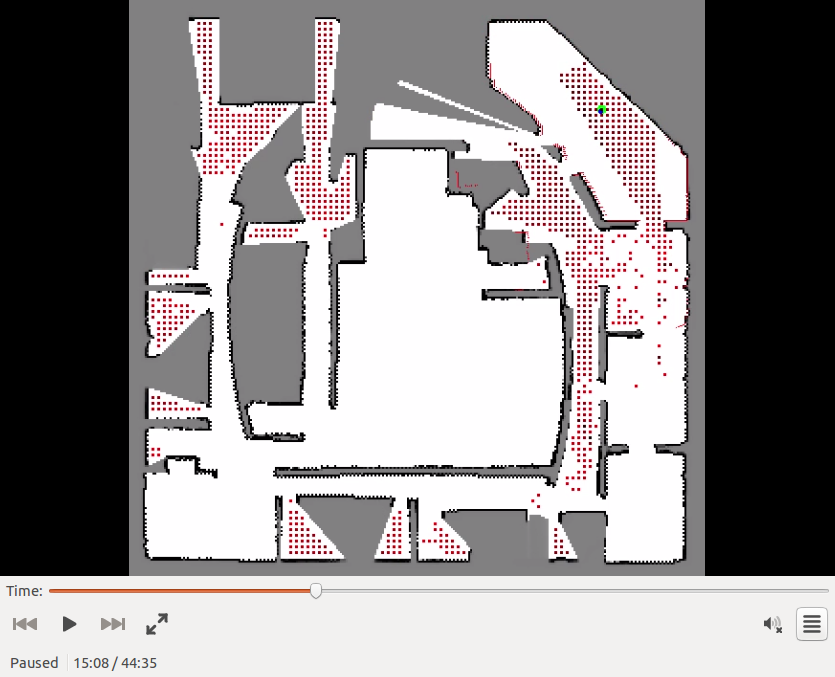
\includegraphics[trim = {4.6cm 3.8cm 4.6cm 0}, clip, width=\textwidth]{15min.png}
        \caption{$t=15$ min}
        \label{fig:IRL15min}
    \end{subfigure}
    \begin{subfigure}[t]{0.3\columnwidth}
         \centering
         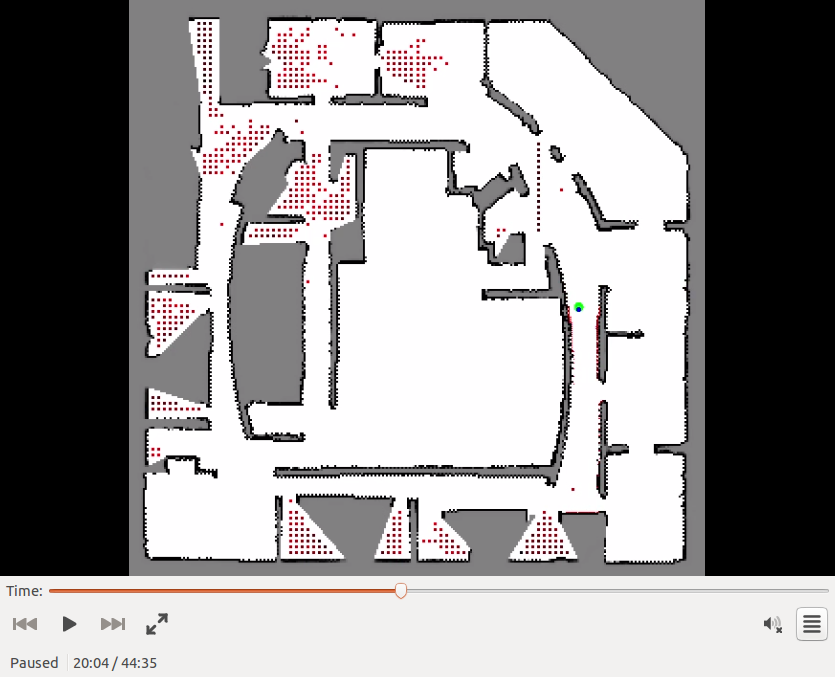
\includegraphics[trim = {4.6cm 3.8cm 4.6cm 0}, clip, width=\textwidth]{20min.png}
        \caption{$t=20$ min}
        \label{fig:IRL20min}
    \end{subfigure}
    \begin{subfigure}[t]{0.3\columnwidth}
           \centering
           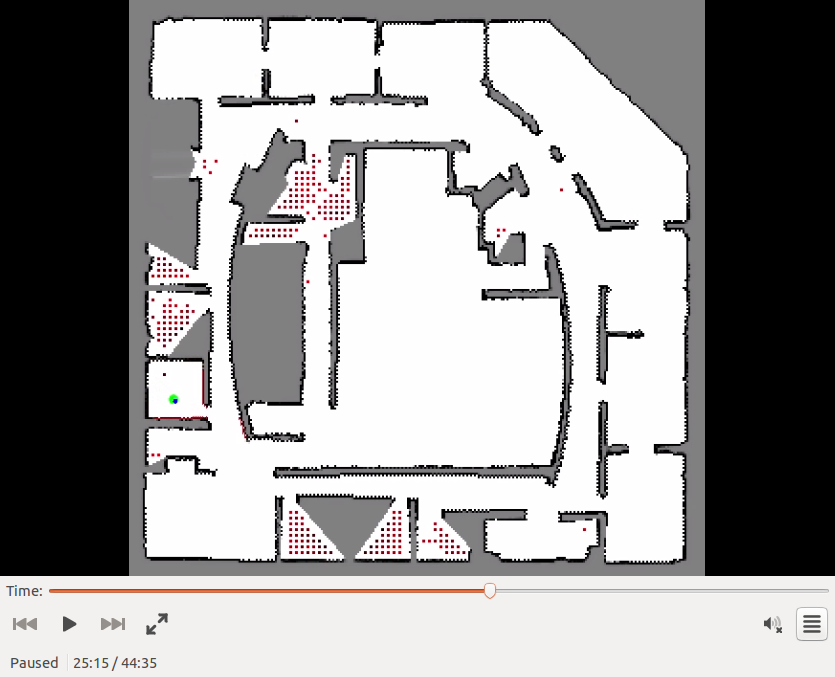
\includegraphics[trim = {4.6cm 3.8cm 4.6cm 0}, clip, width=\textwidth]{25min.png}
        \caption{$t=25$ min}
        \label{fig:IRL25min}
    \end{subfigure}
    \begin{subfigure}[t]{0.3\columnwidth}
           \centering
           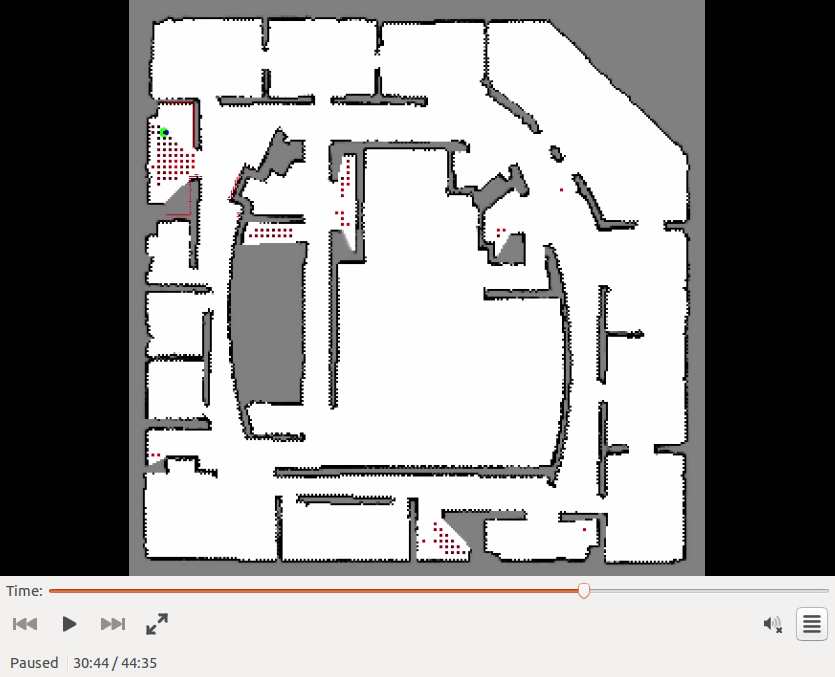
\includegraphics[trim = {4.6cm 3.8cm 4.6cm 0}, clip, width=\textwidth]{30min.png}
        \caption{$t=30$ min}
        \label{fig:IRL30min}
    \end{subfigure}
    \begin{subfigure}[t]{0.3\columnwidth}
           \centering
           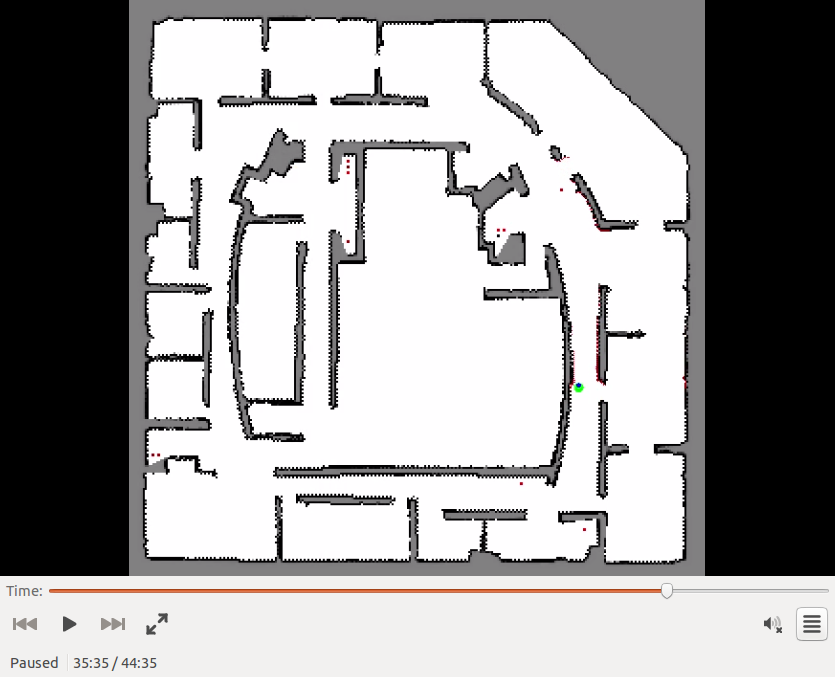
\includegraphics[trim = {4.6cm 3.8cm 4.6cm 0}, clip, width=\textwidth]{35min.png}
        \caption{$t=35$ min}
        \label{fig:IRL35min}
    \end{subfigure}
    \begin{subfigure}[t]{0.3\columnwidth}
           \centering
           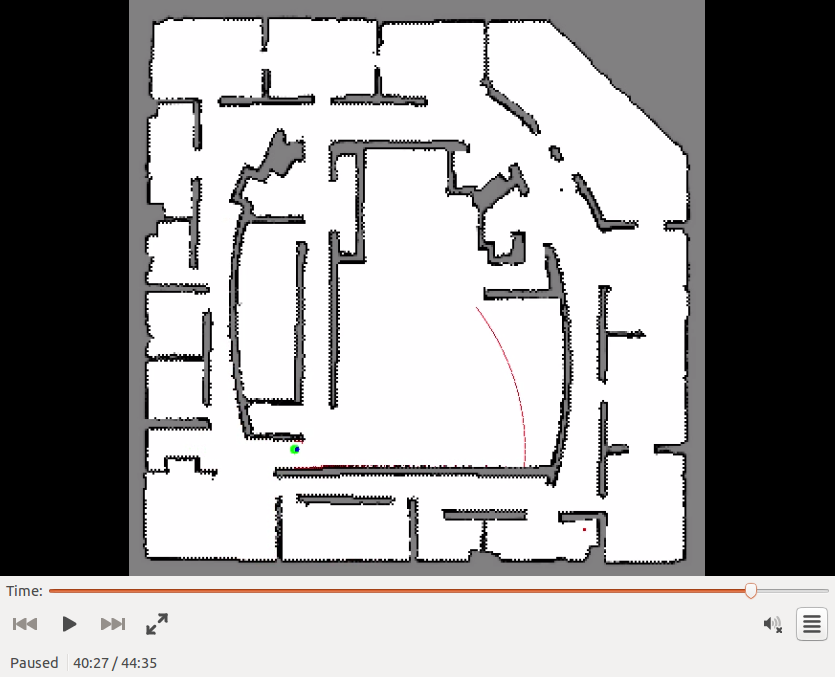
\includegraphics[trim = {4.6cm 3.8cm 4.6cm 0}, clip, width=\textwidth]{40min.png}
        \caption{$t=40$ min}
        \label{fig:IRL40min}
    \end{subfigure}
    \caption{A robot (green) measures a room in ROS Stage simulator using modified Intel Research Lab floor plan. The exact inverse sensor model is used for the autonomous exploration algorithm.}
    \label{fig:IRL}
\end{figure}



%\section{Numerical Examples}
%\label{sec:NumRes}
%
%The efficacy of the proposed algorithms are verified by numerical examples. First, the occupancy grid mapping strategies are simulated in Section \ref{sec:NEOGC}, followed by numerical examples for autonomous exploration in Section \ref{sec:NEAE}. 
%
%% It is common practice to approximate\refeqn{InvSenModWithProbDens} with a simplified function, frequently following the structure of the approximate inverse sensor model proposed in~\cite{And09}. The main idea of this approach is that the probability of a cell being occupied ($i$) near a measurement is high (measurement likely hits this cell), ($ii$) between the robot and the measurement is low (measurement passes through this cell), and ($iii$) beyond the measurement is unchanged (the robot cannot measure through a wall/object). The function is based on intuition, not thorough mathematical derivation. In short, this approach simplifies the inverse sensor model at the cost of accuracy.
%
%%The Kinect depth sensor is used as an example, with specifications from~\cite{KhoElb12}. With these parameters and the identical set of measurements, the exact solution is compared with a benchmark algorithm for a Kinect sensor taken from summarized as follows.
%
%
%
%
%\subsection{Occupancy Grid Mapping}\label{sec:NEOGC}
%
%First, we compare the proposed exact solution to the inverse sensor model summarized in Table \ref{tab:RayByRayISM} with an approximate algorithm presented in~\cite{PirRutBisSch11,KhoElb12}, summarized as follows. The probability that the $i$-th grid cell $\mathbf{m}_i$ is occupied conditioned on the measurement ray $z_{t,l}$ at the pose $X_t$ is the continuous function
%\begin{align*}
%%\label{eqn:ISM_Approx_1}
%&P(\mathbf{m}_i|z_{t,l},X_t)%\nonumber\\&
%=\begin{cases}
%0.3+(\frac{k}{\sigma\sqrt{2\pi}}+0.2)e^{-\frac12\left(\frac{\hat z_{l,i}-z_{t,l}}{\sigma}\right)^2}\ &\text{if}\ \hat z_{l,i} \leq z_{t,l},%z_{t,l}\leq \hat z_{l,i},
%\\
%0.5+\frac{k}{\sigma\sqrt{2\pi}}e^{-\frac12\left(\frac{\hat z_{l,i}-z_{t,l}}{\sigma}\right)^2}\ &\text{otherwise},
%\end{cases}
%\end{align*}
%which is based on the expected distance to the cell $\hat z_{l,i}$ with parameters $k=\sigma=0.6$. This follows the structure of the approximate inverse sensor model proposed in~\cite{And09}. The main idea of this approach is that the probability of a cell being occupied (i) near a measurement is high (measurement likely hits this cell), (ii) between the robot and the measurement is low (measurement passes through this cell), and (iii) beyond the measurement is unchanged (the robot cannot measure through a wall/object). 
%Then, these probabilities are combined in a weighted fashion such that all measurements rays of scan $Z_t$ simultaneously update the same grid cell in a log-odds format,
%\begin{align*}
%%\label{eqn:ISM_Approx_2}
%&\log\left(\frac{P(\mathbf{m}_i|Z_{t},X_t)}{1-P(\mathbf{m}_i|Z_{t},X_t)}\right)
%%\nonumber\\&
%=
%\frac1{\sum_{z_{t,l}\in\mathbf{m}_i}\hat z_{l,i}}\sum_{z_{t,l}\in\mathbf{m}_i}\log\left(\frac{P(\mathbf{m}_i|z_{t,l},X_t)}{1-P(\mathbf{m}_i|z_{t,l},X_t)}\hat z_{l,i}\right).
%\end{align*}
%
%Given the same poses and measurement sets, the proposed algorithm from \refeqn{RayISMAnswer}-\refeqn{RayByRayScanISM} are compared with the approximate algorithm described above. A probabilistic map consisting of NUMX by NUMY square grid cells with edge length ALPHA is assumed to accurately represent the occupancy of the environment surrounding a robot. The robot follows (SOMETHING ABOUT THE TRAJECTORY). With both algorithms, the probabilistic maps are updated in real time.
%
%(PARAGRAPH ABOUT MAP CLARITY, ENTROPY, AND COMPUATION TIME)
%
%%\paragraph{Computation Time}
%%The proposed ray inverse sensor model is designed to maintain the accuracy of the exact solution with substantial computational improvements.
%%A $1$-dimensional example is simulated on a Mac desktop computer with $11$ grid cells, $10$ of which are visible to the robot, where the same depth measurement is used for all occupancy grid algorithms.
%%The computational time of the exact solution is computed in the conventional manner according to \refeqn{InvSenModWithProbDens} in $2.3314$ seconds to obtain the same solution of \refeqn{RayISMAnswer} from \refeqn{Unnormalized} and \refeqn{allEta} in just $0.0027$ seconds, which is $874.77$ times faster.
%%The approximate ray inverse sensor model completes in $0.0011$ seconds, but this algorithm does not follow a forward sensor model, so the probabilities of the map may be inaccurate.
%
%
%
%
%
%
%
%
%%\subsection{Trajectory Map Building}
%%In this numerical example, we consider a robot in a two-dimensional environment composed of ten wall edges, and the robot follows a figure-eight curve, then turns around and completes the same curve in the reverse direction.
%%The map is composed of $100\times100$ square grid cells with edge length of $1$ cm.
%%A forward sensor model $p(z_t|m,X_t)$~\cite{ThrBurFox05} is constructed according to the specifications of the Kinect sensor~\cite{KhoElb12}, and a pseudo-random measurement scan is sampled at each time step via the inverse transform sampling~\cite{DevBK86}. The same set of measurements updated each second are used with both occupancy grid mapping algorithms to construct the map.
%%
%%The resulting maps are illustrated in Figure \ref{fig:NumResOccProbs} for both algorithms, where it is shown that the proposed algorithm yields a substantially more accurate and clear map with less uncertainty. To quantify the degree of map uncertainty, we define the entropy of the map as 
%%\begin{align*}
%%&H(P(m|X_{1:t},Z_{1:t}))=\nonumber\\
%%&-\sum_{i=1}^n\big\{P(\mathbf{m}_i|X_{1:t},Z_{1:t})\log P(\mathbf{m}_i|X_{1:t},Z_{1:t})\nonumber\\
%%&+(1-P(\mathbf{m}_i|X_{1:t},Z_{1:t}))\log(1-P(\mathbf{m}_i|X_{1:t},Z_{1:t}))\big\},
%%\end{align*}
%%which is maximized when the probability of occupancy is $0.5$ for all cells (more uncertain), and it is minimized when they are either $0$ or $1$ (less uncertain). 
%%
%%The change of the map entropy over time, and the entropy of the completed maps, for both methods are depicted in Figure \ref{fig:NumResOccH}. The subfigure (a) illustrates that the proposed exact inverse sensor model exhibits rapid decreases of entropies, and smaller entropies always. The resulting terminal map obtained from the proposed approach, shown in the subfigure (b), has less uncertainty than (c) constructed by the approximate model. In short, the proposed approach is more efficient at extracting information about the environment from the same set of set measurements. 
%
%
%
%
%
%
%\subsection{Autonomous Exploration}\label{sec:NEAE}
%
%%Maximizing the proposed expected information gain serves as the objective for autonomous exploration. A robot begins in a completely uncertain environment, except for the grid cells inside the immediate vicinity the robot location. 
%
%WILL UPDATE ONCE RESULTS ARE BETTER
%The robot explores its surroundings with an occupancy grid with $15000$ cells where grid cell edges are $\alpha=0.2$m, composing a map with dimensions $30\text{m}\times20\text{m}$. The initial probability $P(\mathbf{m}_i)=1\times10^{-10}\approx0$ (minimum value for free space) for grid cells covered by the circular robot of radius $0.1$m and $P(\mathbf{m}_i)=0.5$ for all other cells.
%At each time step, the robot receives a measurement scan, where the probabilistic properties of the sensor are taken from~\cite{PirRutBisSch11,KhoElb12}. Then, the $n_c=8$ evenly-spaced candidate locations about a circle of radius $\delta=0.5$m around the current pose location are considered, where $n_d=32$ measurement rays are evenly-spaced about the candidate location.  When no current candidates yield expected information gains above $\mathcal I_\text{min}=2$, $\lambda=1.25$ is multiplied to the current $n_c$ and $\delta$ values. The motion of the robot is restricted to movement on grid cells satisfying \refeqn{CollisionInequalityConstraint} with $\beta=0.01$. Dijkstra's algorithm guides the robot through the environment without collision. The results are illustrated in Figure \ref{fig:AutonomousExploration}.


\section{Experimental Results}
\label{sec:ExpRes}
	% Kinect result

%A preliminary experiment shows how the exact inverse sensor model is successfully implemented with the Kinect sensor.



The efficacy of the proposed mapping and autonomous exploration algorithms are also verified with experiments. The experiment involves a ground vehicle producing a probabilistic occupancy grid map in real time. The robot motion is governed by the information gain-maximizing policy described in this paper.

\paragraph{Hardware Configuration}
The Pioneer 3 ground robot was chosen. The vehicle accepts two inputs, namely linear velocity (aligned with the robot wheels) and angular velocity (about a central axis passing vertically through the robot). The robot pose was estimated via Vicon Tracker, which provides the location and attitude of a rigid body. The depth readings were obtained by a Kinect depth sensor. Since the experiment was to map and explore a 2D environment, only a single central row of the 3D Kinect depth scan provided the necessary measurements.
An environment with features of walls and obstacles was constructed by Styrofoam.

\paragraph{Software Configuration}
The proposed algorithm was implemented with ROS. The ROS framework provided seamless communication betweens sensors and actuators, and the executable programs (referred to as ``nodes'') operate quickly when compiled from C++ code. The robot and map are plotted using ``OpenGL'' libraries.

Synchronization between the sensors is of high importance to the proposed occupancy grid mapping approach. Any time delay between the robot pose estimation and the sensor depth readings can cause conflicting information, which may be harmful to the probabilistic map. Thus, ROS approximate message filters were applied such that the pose from Vicon Tracker ($100$Hz) and the Microsoft Kinect ($30$Hz) were nearly synchronized, which provided validity of the assumption that the measurement ray positions and directions are known deterministically.

\paragraph{Exploring and Mapping a 2D Environment}
The environment consisted of Styrofoam walls on a flat floor. The parameter was oriented in a rectangle, with several obstacles and angled walls (see Figure \ref{fig:ExpSetupPhoto}). The robot autonomously explored the space using the complete Cartesian searching approach, and Dijkstra's algorithm provided collision-free waypoints to the optimal future poses. Based on these waypoints, a constrained least squares polynomial fitting method provided a smooth trajectory to follow the waypoints with fixed velocity. Finally, a simple controller was implemented such that the Pioneer moved along the trajectory by moving and orienting toward the desired robot location $1$sec in the future.

\begin{figure}
	\centering
    	\begin{subfigure}[b]{0.35\textwidth}
        		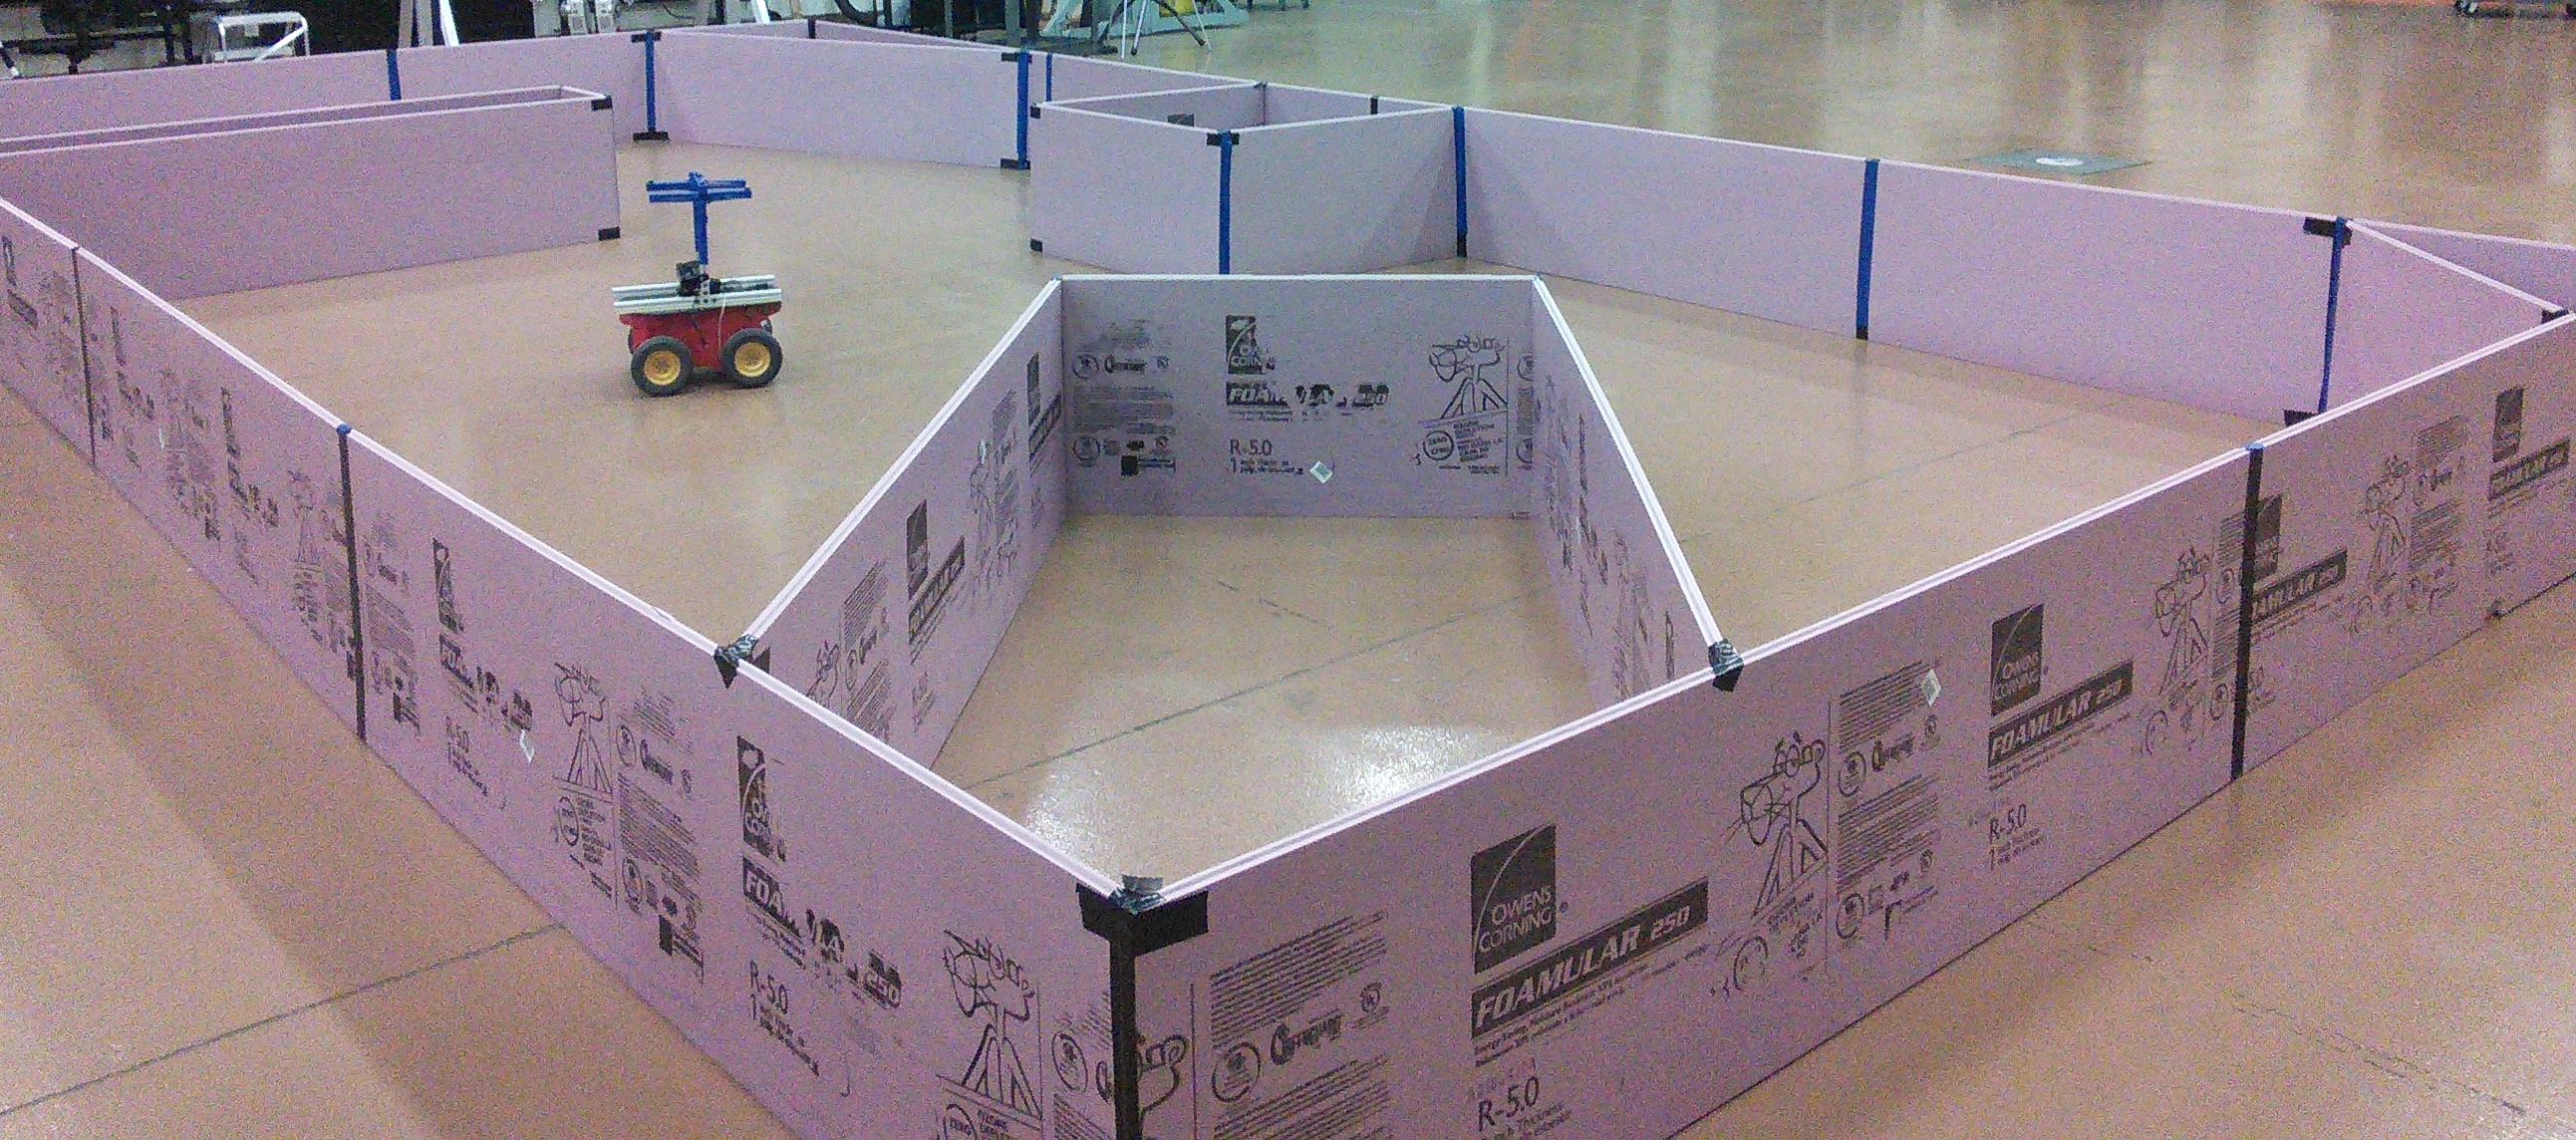
\includegraphics[width=\textwidth]{test_setup_bottom_left_cropped.jpg}
        		\caption{Bottom-left view}
        		\label{fig:Experiment_blv}
    	\end{subfigure}
	\hspace*{0.05\columnwidth}
	\begin{subfigure}[b]{0.35\textwidth}
        		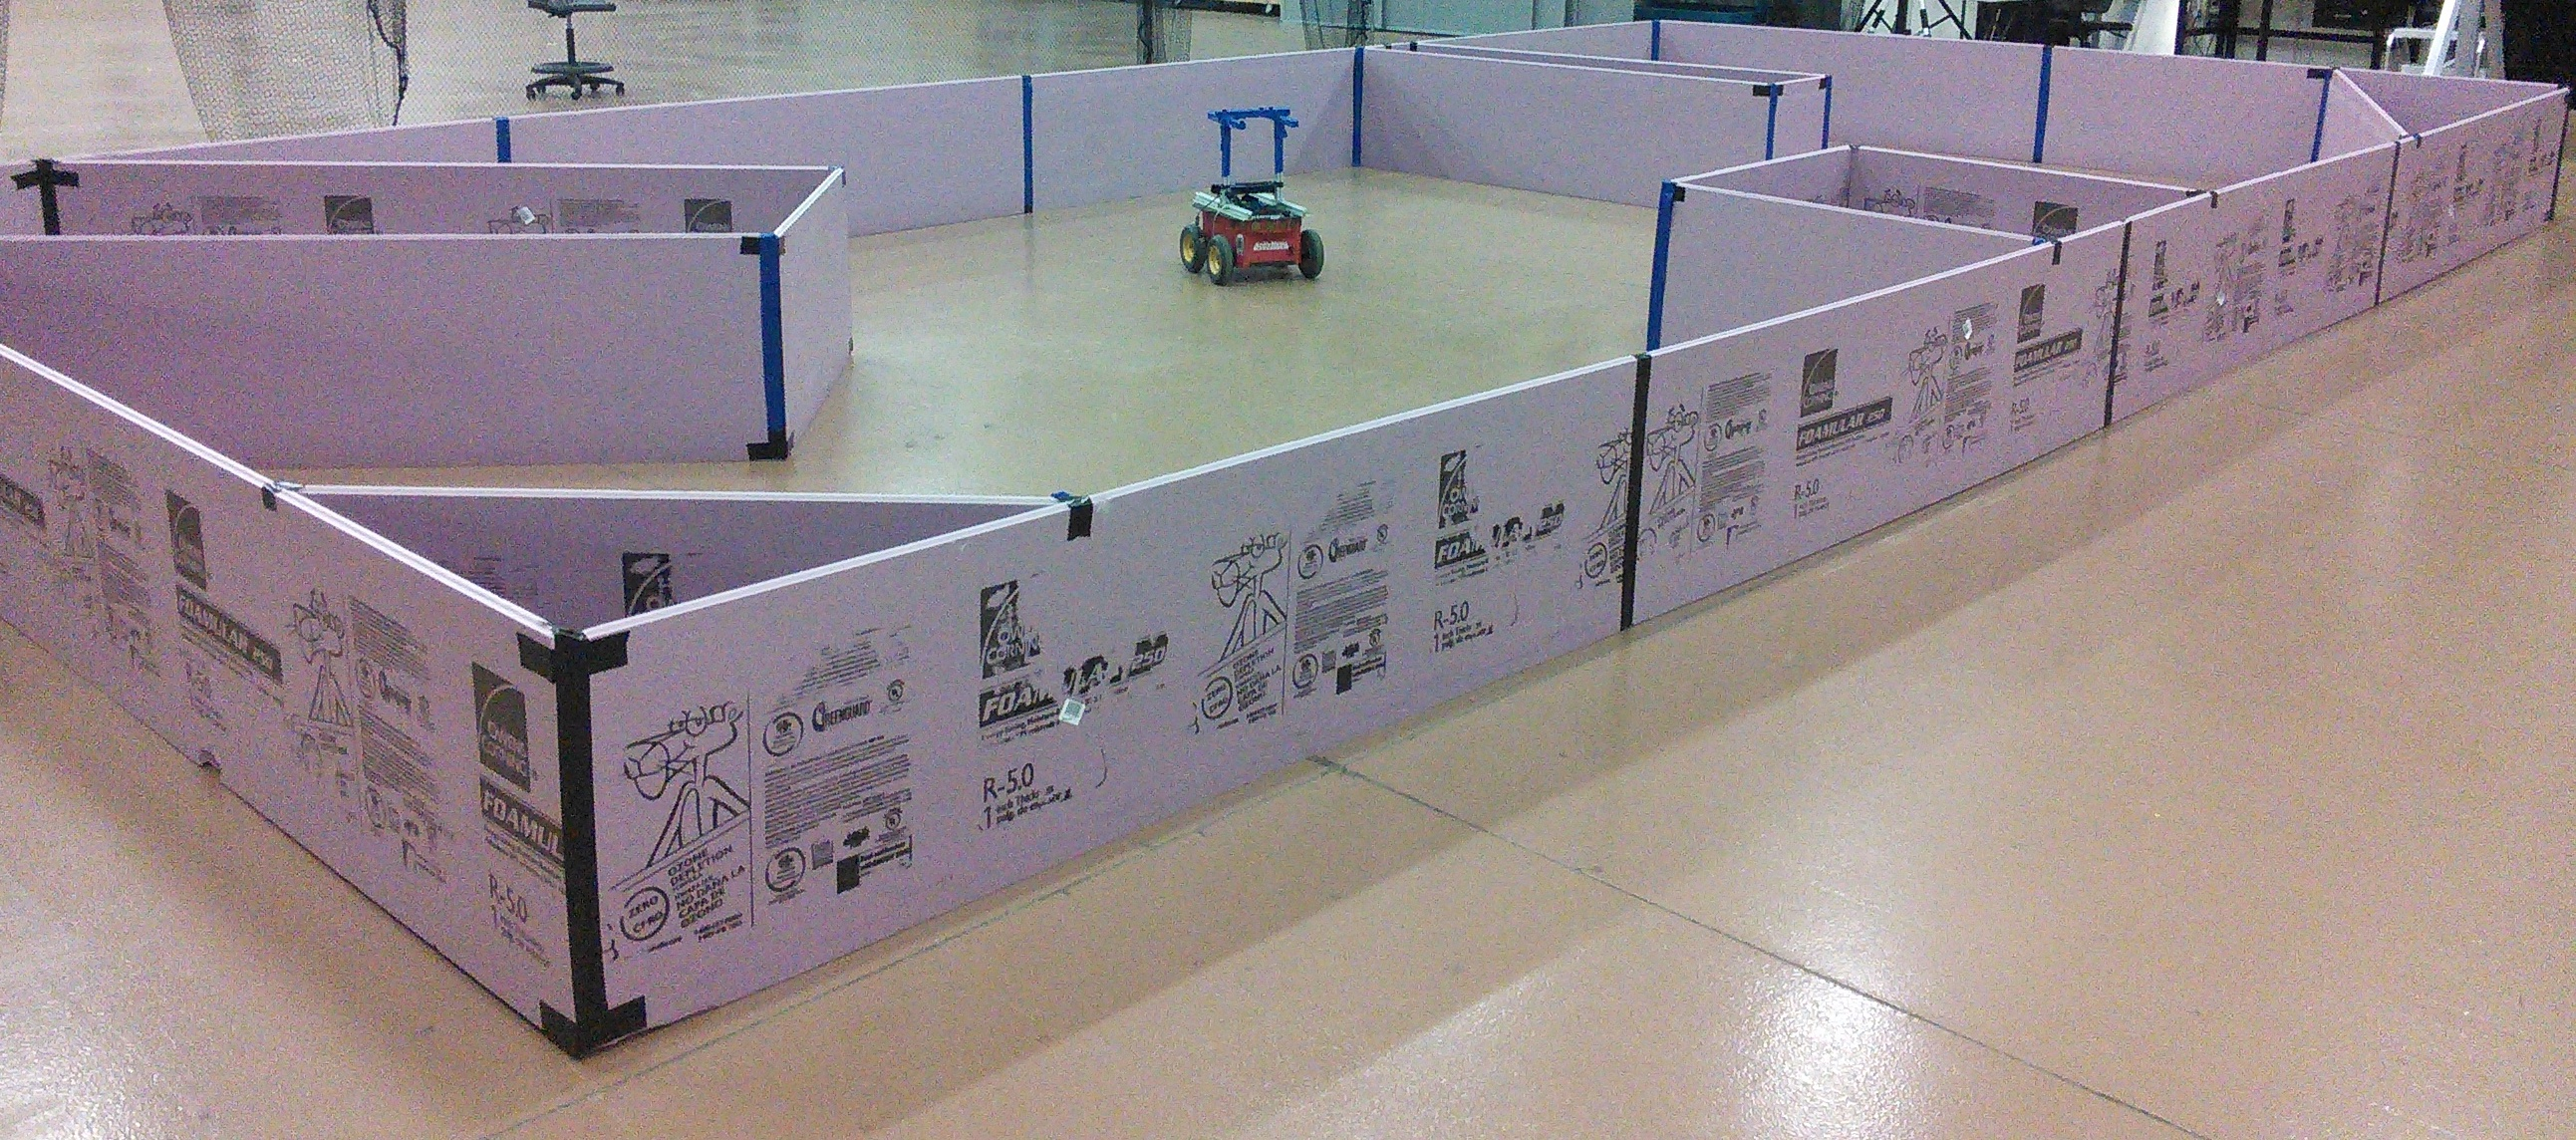
\includegraphics[width=\textwidth]{test_setup_bottom_right_cropped.jpg}
        		\caption{Bottom-right view}
        		\label{fig:Experiment_brv}
    	\end{subfigure}
\caption{Images from two perspectives show the walls and obstacles of the experimental environment.}
\label{fig:ExpSetupPhoto}
\end{figure}


The resulting occupancy grid maps and trajectories are depicted in Figure \ref{fig:ExperimentOGM} and a video is available at \href{https://www.youtube.com/watch?v=CRQfhhICSj0&feature=youtu.be}{\WriteBlue{www.youtube.com/watch?v=CRQfhhICSj0\&feature=youtu.be}}. Most importantly, the robot builds a clear occupancy grid map despite sensor noise and imperfect sensor synchronization. The autonomous exploration successfully guides the robot such that it builds a map of the reachable space without colliding with any obstacles.


\begin{figure}
	\centering{
    	\begin{subfigure}[b]{0.19\textwidth}
        		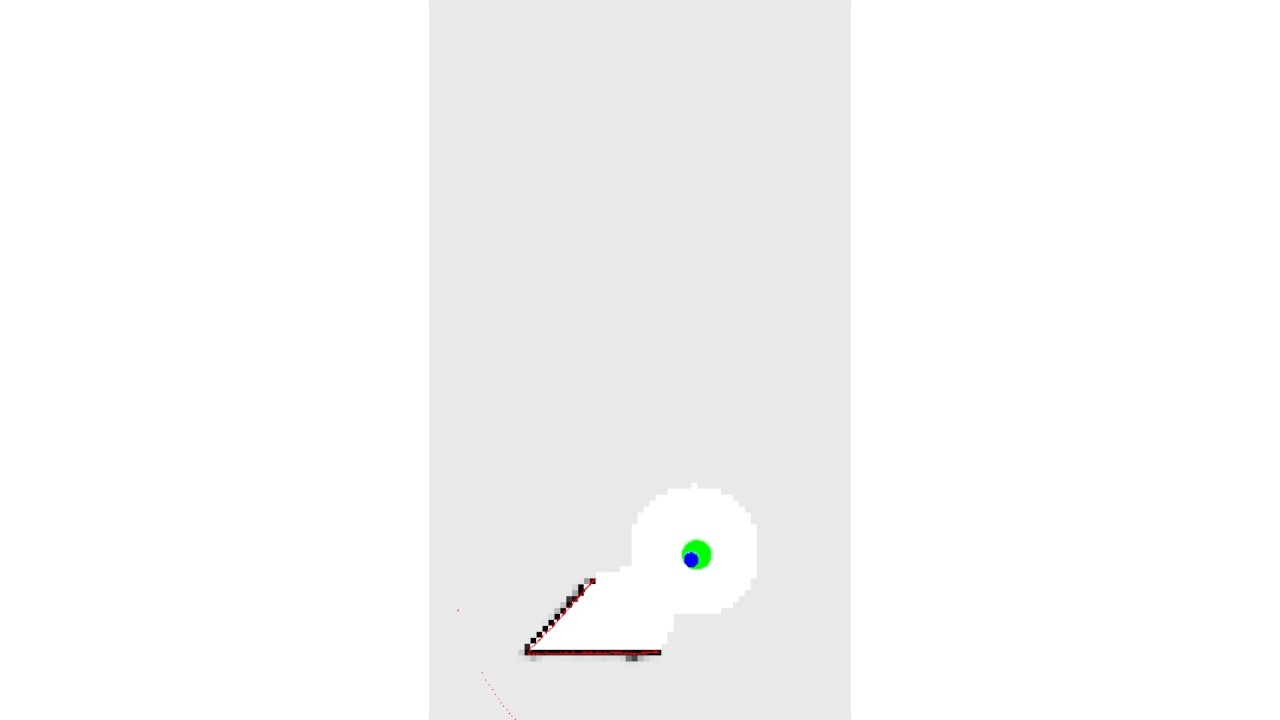
\includegraphics[trim={13cm 1cm 13cm 0}, clip, width=\textwidth]{feb23_t0sec.jpg}
        		\caption{$t=0$sec}
        		\label{fig:Experiment_ogm_t0}
    	\end{subfigure}
	\begin{subfigure}[b]{0.19\textwidth}
        		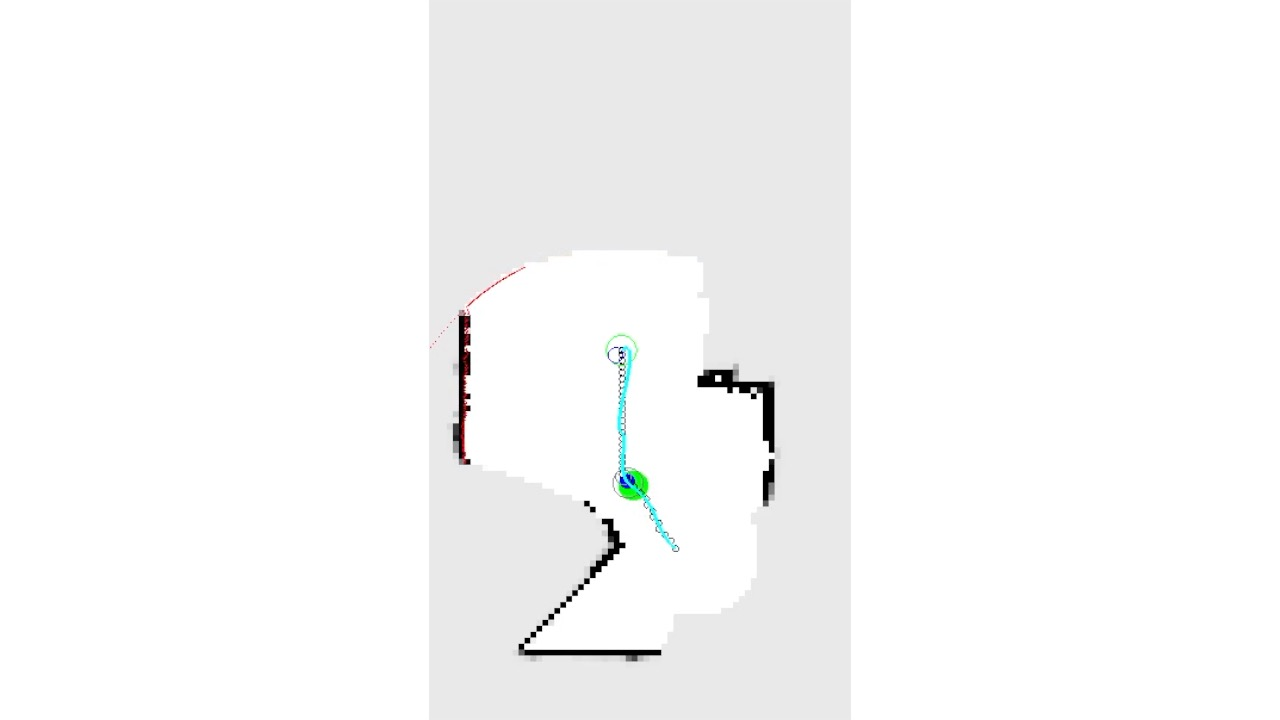
\includegraphics[trim={13cm 1cm 13cm 0}, clip, width=\textwidth]{feb23_t20sec.jpg}
        		\caption{$t=20$sec}
        		\label{fig:Experiment_ogm_t0p5}
    	\end{subfigure}    
	\begin{subfigure}[b]{0.19\textwidth}
        		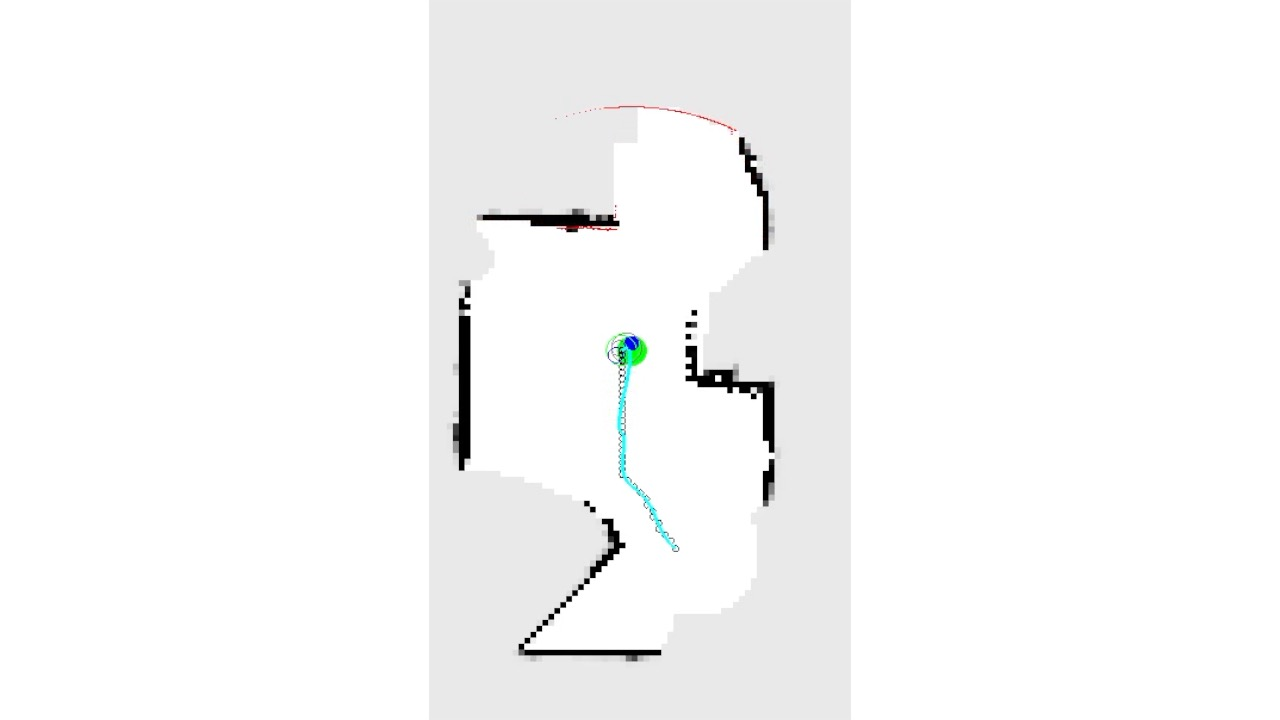
\includegraphics[trim={13cm 1cm 13cm 0}, clip, width=\textwidth]{feb23_t40sec.jpg}
        		\caption{$t=40$sec}
        		\label{fig:Experiment_ogm_t1}
    	\end{subfigure}
	\begin{subfigure}[b]{0.19\textwidth}
        		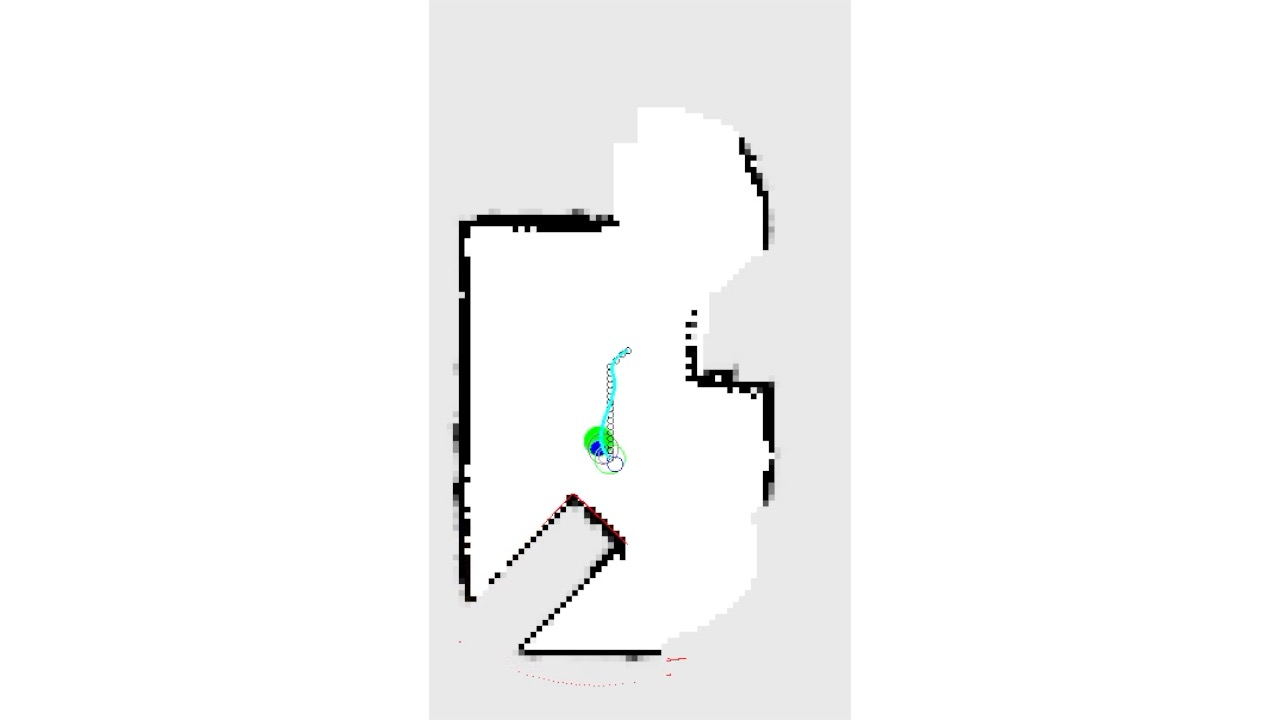
\includegraphics[trim={13cm 1cm 13cm 0}, clip, width=\textwidth]{feb23_t60sec.jpg}
        		\caption{$t=60$sec}
        		\label{fig:Experiment_ogm_t1p5}
    	\end{subfigure}
	\begin{subfigure}[b]{0.19\textwidth}
        		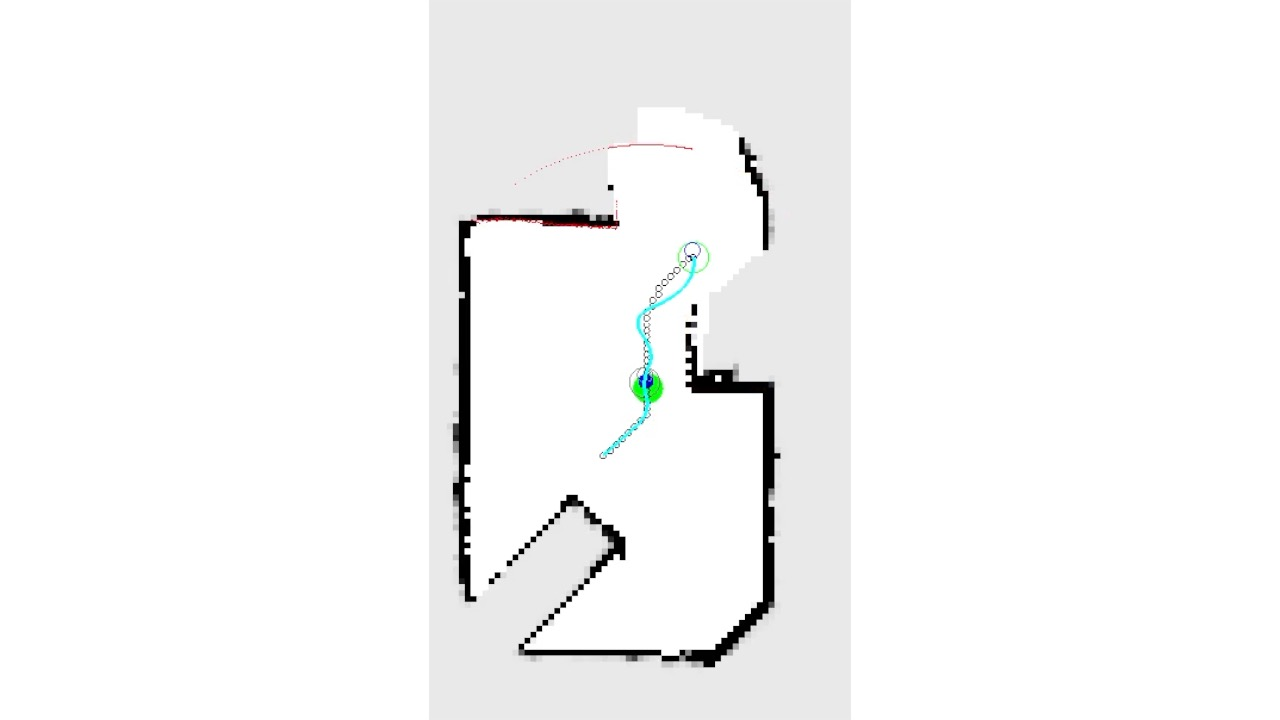
\includegraphics[trim={13cm 1cm 13cm 0}, clip, width=\textwidth]{feb23_t80sec.jpg}
        		\caption{$t=80$sec}
        		\label{fig:Experiment_ogm_t2}
    	\end{subfigure}
		\vspace*{0.05\textwidth}

	}
	\centering{
    	\begin{subfigure}[b]{0.19\textwidth}
        		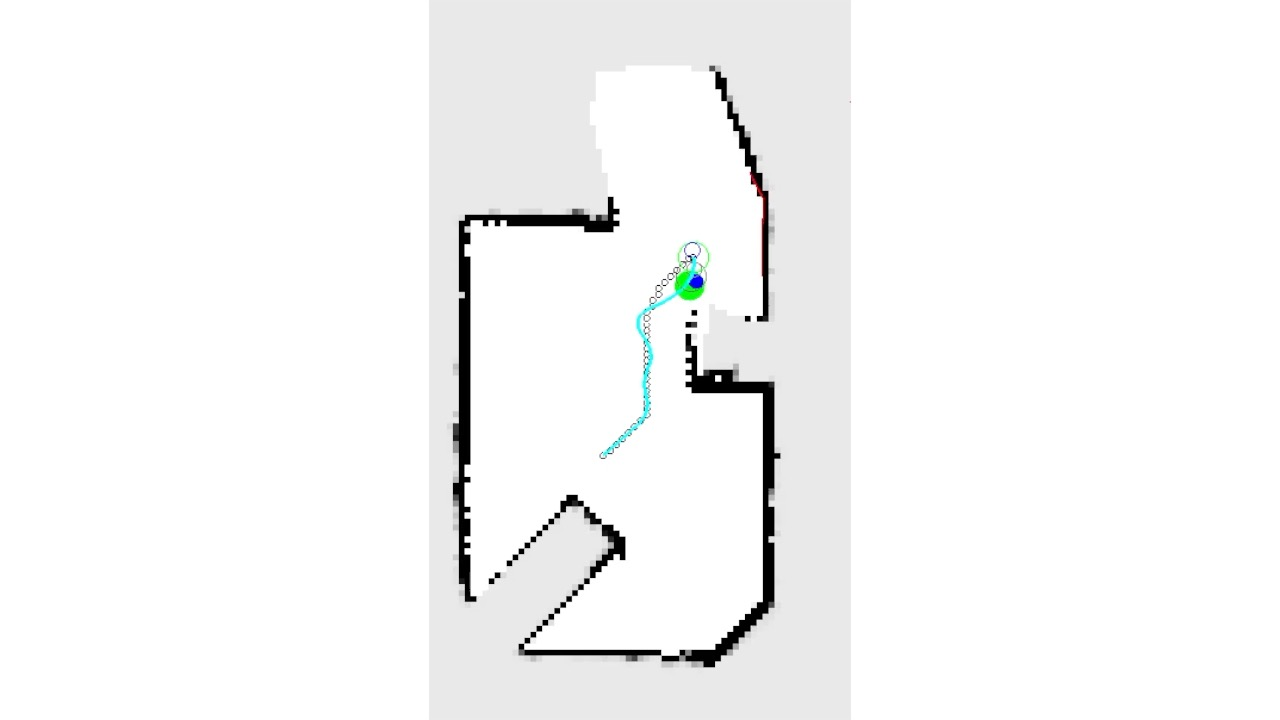
\includegraphics[trim={13cm 1cm 13cm 0}, clip, width=\textwidth]{feb23_t100sec.jpg}
        		\caption{$t=100$sec}
        		\label{fig:Experiment_ogm_t2p5}
    	\end{subfigure}
	\begin{subfigure}[b]{0.19\textwidth}
        		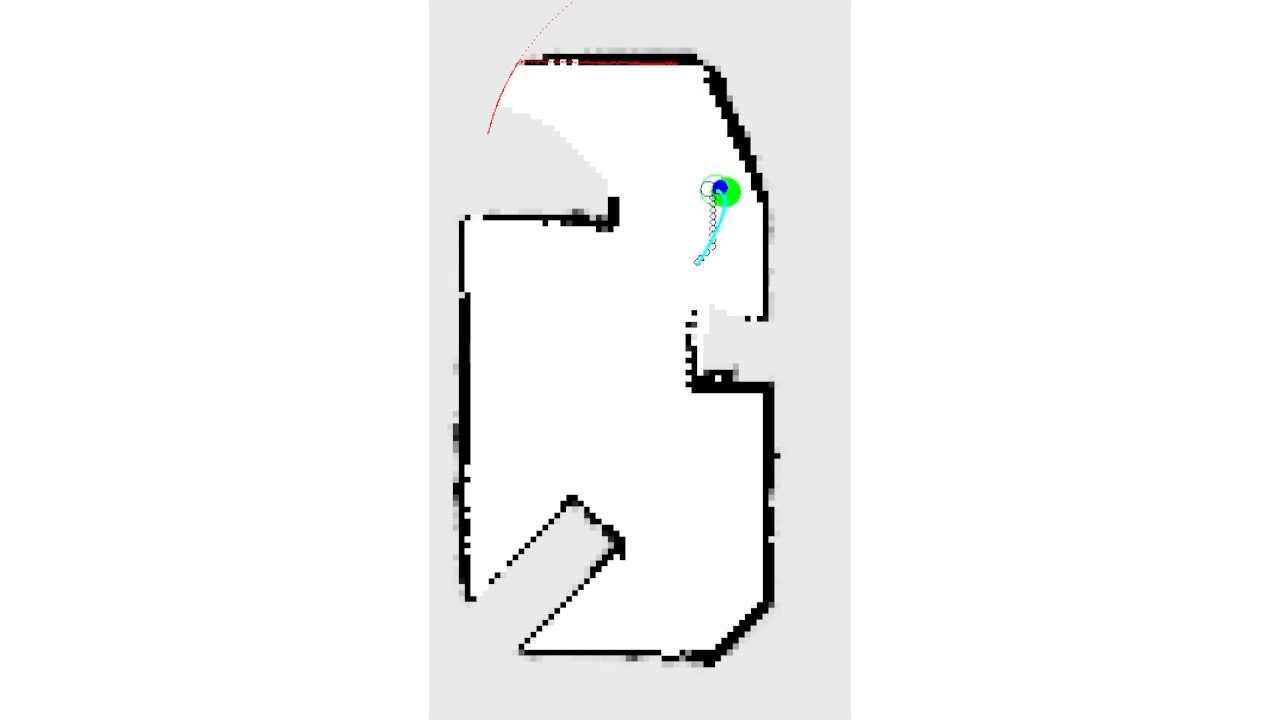
\includegraphics[trim={13cm 1cm 13cm 0}, clip, width=\textwidth]{feb23_t120sec.jpg}
        		\caption{$t=120$sec}
        		\label{fig:Experiment_ogm_t3}
    	\end{subfigure}    
	\begin{subfigure}[b]{0.19\textwidth}
        		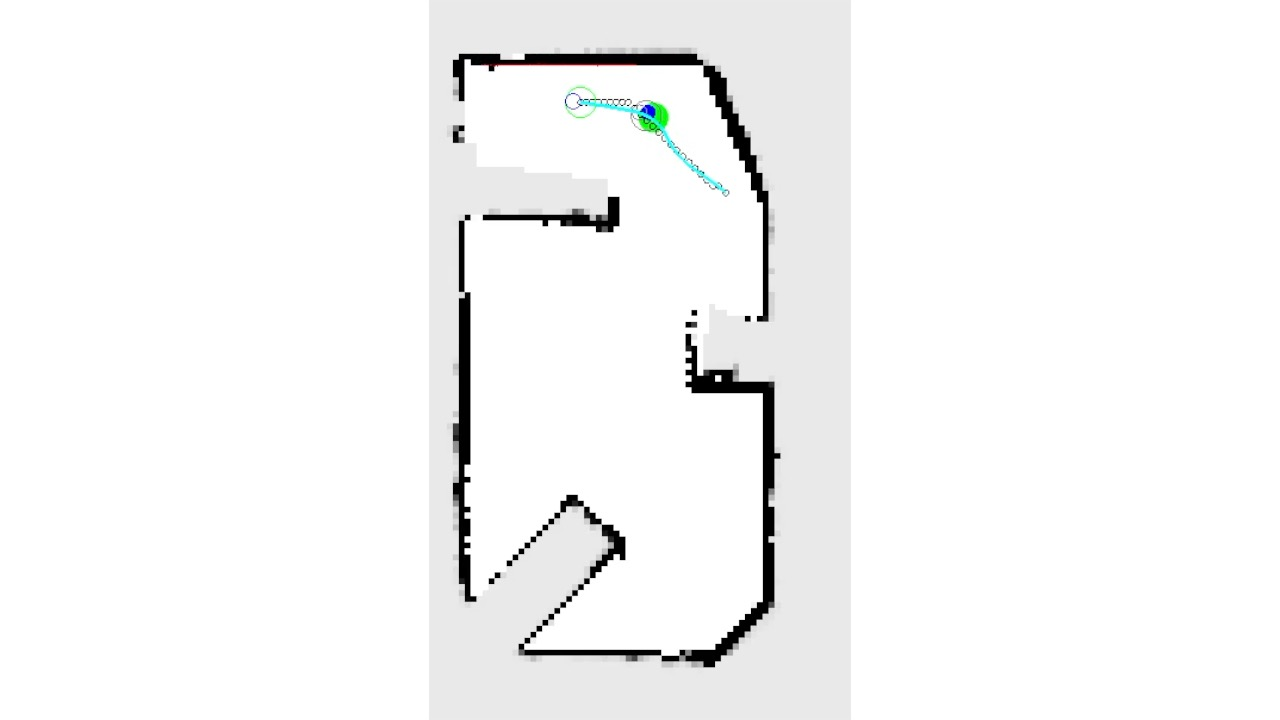
\includegraphics[trim={13cm 1cm 13cm 0}, clip, width=\textwidth]{feb23_t140sec.jpg}
        		\caption{$t=140$sec}
        		\label{fig:Experiment_ogm_t3p5}
    	\end{subfigure}
	\begin{subfigure}[b]{0.19\textwidth}
        		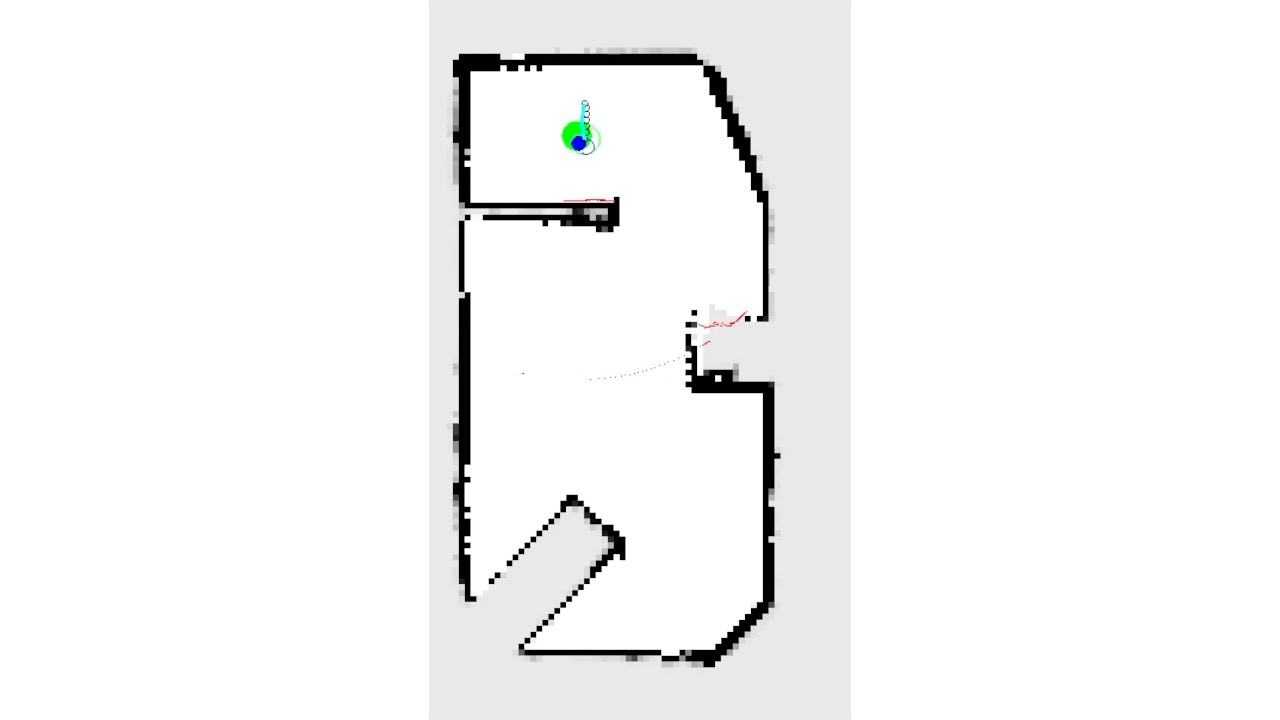
\includegraphics[trim={13cm 1cm 13cm 0}, clip, width=\textwidth]{feb23_t160sec.jpg}
        		\caption{$t=160$sec}
        		\label{fig:Experiment_ogm_t4}
    	\end{subfigure}
	\begin{subfigure}[b]{0.19\textwidth}
        		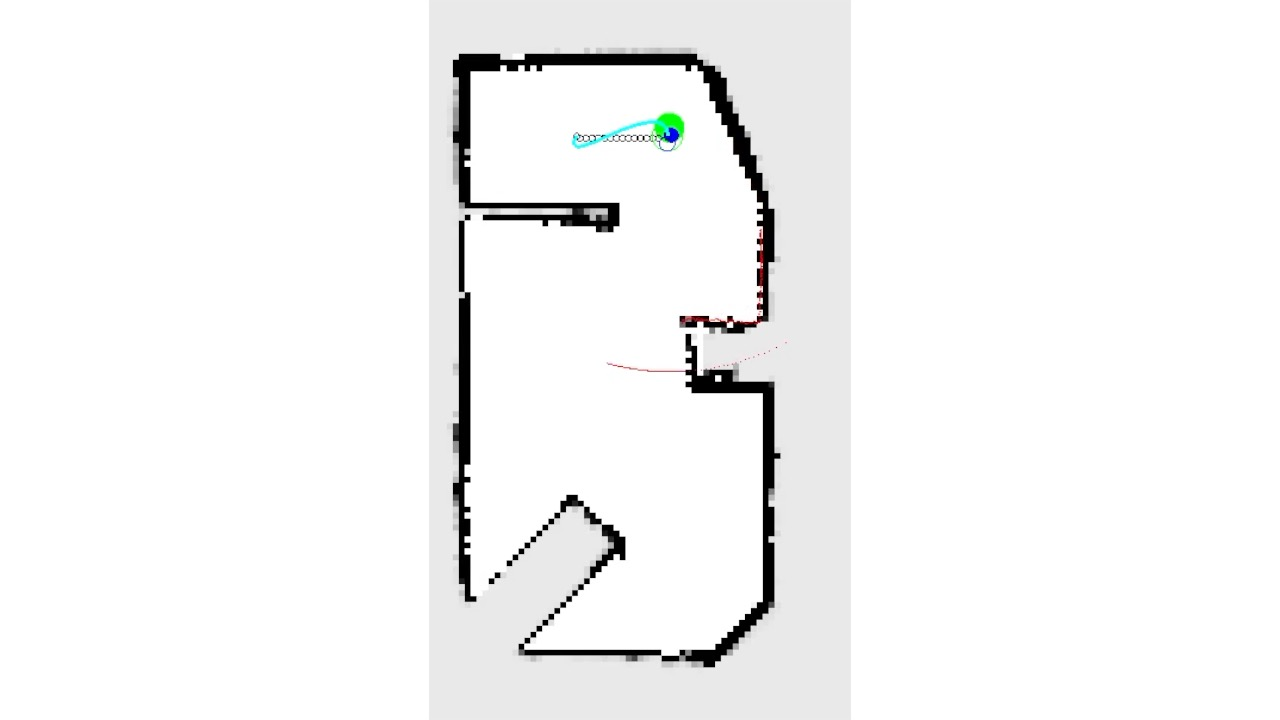
\includegraphics[trim={13cm 1cm 13cm 0}, clip, width=\textwidth]{feb23_t180sec.jpg}
        		\caption{$t=180$sec}
        		\label{fig:Experiment_ogm_t4p5}
    	\end{subfigure}
	}
\caption{A robot autonomously explores the experimental environment and produces an occupancy grid map along the way. The robot (shaded green circle body with shaded blue circle sensor) is controlled toward the desired pose $1$sec in the future (unshaded grey robot), which is following a constrained least-squares trajectory (cyan curve). This trajectory is based on waypoints (black circles) from Dijkstra's algorithm to arrive at the optimal pose (unshaded green circle body with unshaded blue circle sensor) as proposed in this paper.}
\label{fig:ExperimentOGM}
\end{figure}

%The resulting map and exploration commands are generated in real time. The grid cells are stored as double-float variables in a vector, where the vector index is mapped to a location on the occupancy grid. Thus, the memory requirements are proportional to the number of grid cells, which is roughly the mapping area divided by the area of a grid cell. Since cell locations need not be saved, memory requirements are reduced. The mean time for updating the occupancy grid is $0.0115$ seconds, and the mean time to determine an exploration strategy is $0.6820$ seconds. Time requirements for mapping and exploration are easily modified by changing grid cell resolution or the number of exploration pose candidates, respectively. In short, there is a tradeoff between computational speed and accuracy of mapping or exploration.
The resulting map and exploration commands are generated in real time. The grid cells are stored as double-float variables in a vector, where the vector index is mapped to a location on the occupancy grid. Thus, the memory requirements are proportional to the number of grid cells, which is roughly the mapping area divided by the area of a grid cell. Since cell locations need not be saved, memory requirements are reduced. On a Lenovo T540p laptop with an Intel Core i7-4900MQ processor (quad-core, 2.8GHz per core) and 16GB of RAM, the mean time for updating the occupancy grid is $0.0115$ seconds, and the mean time to determine an exploration strategy is $0.6820$ seconds. Time requirements for mapping and exploration are easily modified by changing grid cell resolution or the number of exploration pose candidates, respectively. In short, there is a tradeoff between computational speed and accuracy of mapping or exploration.

The autonomous exploration is governed by a policy to maximize expected entropy decreases, so entropy and entropy change with time (Figure \ref{fig:ExperimentH}) are important metrics. In this example, the a priori occupancy probabilities of all cells are $0.1$, so the entropies could temporarily rise for likely occupied cells. The total map entropy begins at roughly $2613$ and decreases by roughly half to $1338$. Many grid cells within the map limits are occluded by walls, preventing the blocked cells from occupancy probability changes. In some cases, the robot is able to update the cell occupancy probabilities; in other cases, cells fall inside regions occluded from all reachable space, and the robot cannot update these cells. Among those grid cells visible from collision-free locations, the vast majority of cells were updated in less than $3$min while following a very slow ($5$cm/sec) trajectory.

Both the numerical and experimental results demonstrated successful exploration strategies, though the algorithm can be improved. In particular, the robot sometimes revisits spaces that it has explored before, most frequently when the robot did not take measurements toward a particular direction. A few methods to improve this issue are treated as future work. One options is adding cost functions (e.g. distance based, number of past measurements inside an area) to prevent the robot from leaving an area before it is well-known. A second option is partitioning the space into sections, where the robot moves toward sections with large numbers of pose candidates with high expected information gains. Another option is reevaluating the future pose optimization while the robot is translating between poses because the occupancy grid map is changing, and so is expected information gain. The efficacy of these proposed changes will be evaluated, particularly as they relate to more useful systems, such as 3D map generation and multi-robot exploration.

%Additionally, even though the walls appear fairly well-defined, they are not perfectly straight boundaries. The occupancy grid assumptions do not perfectly align with the true environment; an edge of a wall might occupy only part of a grid cell. Therefore, some measurement rays passing through this cell provide evidence that the cell is free, whereas other rays might provide conflicting evidence that the cell is occupied. Furthermore, any error in robot attitude estimation can degrade the map; an attitude error of $1^{\circ}$ corresponds to an offset of $11$ measurement rays propagating across the $640$ measurement rays composing the Kinect depth scan.

\begin{figure}
	\centering
	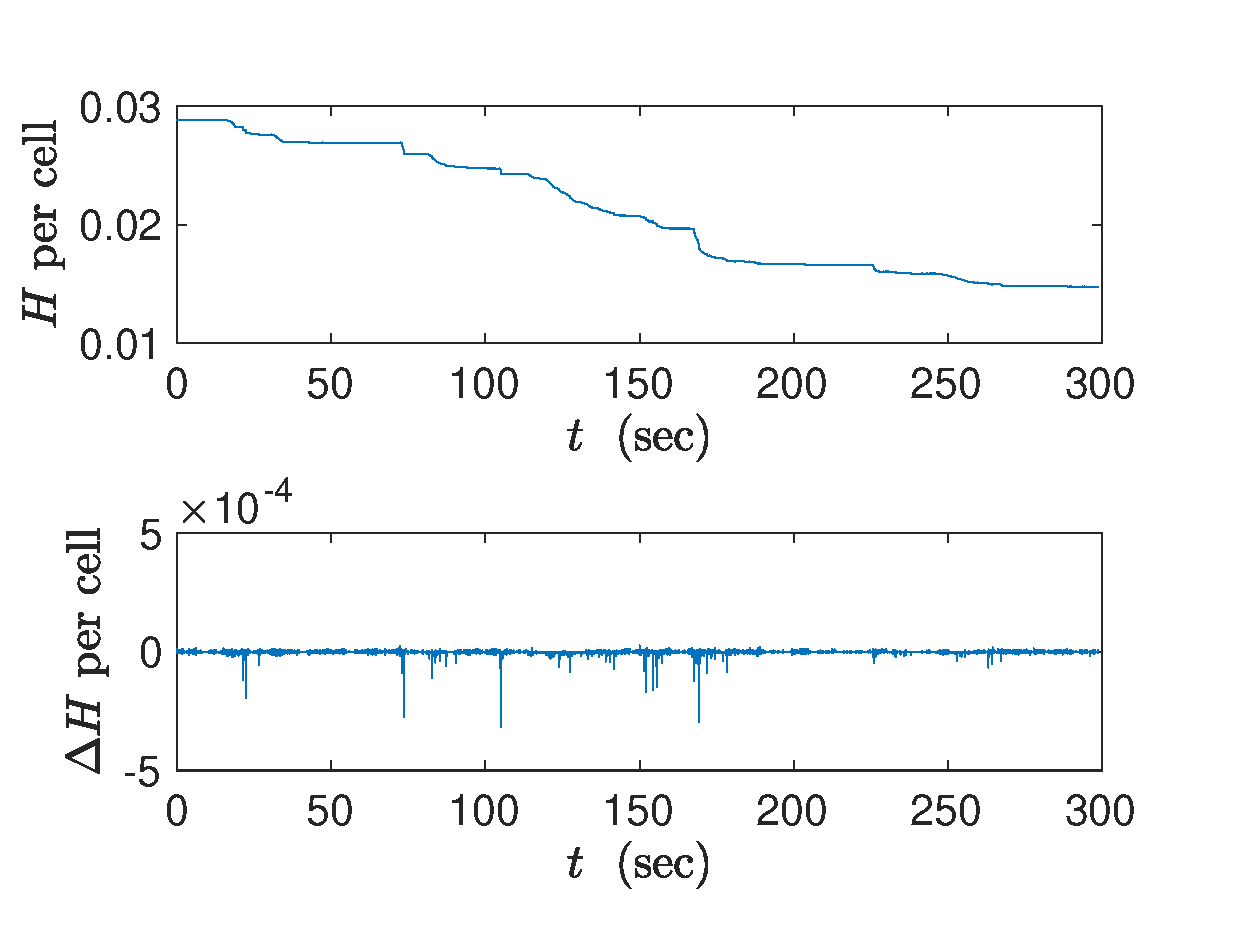
\includegraphics[width=\textwidth]{JIRS_fig11.eps}
	\caption{The map entropy $H$ averaged over all $90601$ grid cells is reduced during experimentation. The quick changes $\Delta H$ per cell correspond to map updates when the robot captures new territory.}
\label{fig:ExperimentH}
\end{figure}
















\section{Conclusions}
\label{sec:Conclusion}

This paper serves to improve the accuracy occupancy grid mapping and the policy governing robotic motion during autonomous exploration.
With other approaches, each probability of an occupancy grid map is approximated in practice due to the perceived complications of the exact solution.
This paper provides an exact solution to this complicated probability problem using cell occlusion in the forward sensor model. This yields a substantially simpler inverse sensor model, which avoids a potentially harmful Markov assumption that commonly appears in the log-odd ratio formulations. The main contribution of this paper is that all of the information available in the measurements and the a priori estimate is extracted and integrated to generate a more accurate a posteriori map. The numerical and experimental results show that maps using this exact approach are substantially improved. 

The exact probabilistic occupancy grid mapping framework is utilized in autonomous exploration. The robot pose is chosen to minimize the expected map information gain, which is now directly solved more precisely in an unprecedented way. Unlike common techniques based on finding frontiers or predicting measurement scans with particle filters, the proposed approach is based on an expected value of the entropy directly. The approach is approximated with large improvements in computation and small losses in accuracy. Numerical examples and an experiment show how robots navigate uncertain maps governed by the proposed autonomous exploration algorithm while building accurate probabilistic maps.














\section*{Appendix}\label{append}


\subsection*{Proof of Proposition 1}

\paragraph{Unnormalized Reduced Map Inverse Sensor Model}
For the reduced map of the $l$-th ray from \refeqn{InvSenModWithProbDens}, the unnormalized part corresponding to terms without $\eta_{t,l}$ in \refeqn{RayISMAnswer} is %given by
\begin{align}
\tilde P(\mathbf{r}_{l,k}|z_{t,l},X_{1:t},Z_{1:t-1})%\nonumber\\
= \sum_{r\in\mathcal{M}_{k}} p(z_{t,l}|r,X_t) P(r|X_{1:t-1},Z_{1:t-1}).\label{eqn:tildePlk}
\end{align}
Recall $\mathcal{M}_k$ corresponds to the set of maps where the $k$-th cell is occupied. Define a subset $\mathcal{N}_{i,k}\subset \mathcal{M}_k$ for $1\leq i\leq k$ be the set of maps where the $i$-th cell is the first occupied cell. More explicitly, 
\begin{align*}
\mathcal{N}_{i,k}  = \{ r\in\mathcal{M}_k| \mathbf{r}_{l,i+}\}
= \{ r\in\mathcal{M}_k| \mathbf{r}_{l,1}=0,\ldots, \mathbf{r}_{l,i-1}=0, \mathbf{r}_{l,i}=1,
\mathbf{r}_{l,k}=1\}.
\end{align*}
Then, $\mathcal{M}_k$ can be written as $\mathcal{M}_k =\bigcup_{i=1}^{k} \mathcal{N}_{i,k}$. Using this, the summation over $\mathcal{M}_k$ at \refeqn{tildePlk} can be decomposed of the summation over each $\mathcal{N}_{i,k}$ to obtain
\begin{align*}
\tilde P(\mathbf{r}_{l,k}|z_{t,l},X_{1:t},Z_{1:t-1}) = \sum_{i=1}^k\braces{\sum_{r\in\mathcal{N}_{i,k}} p(z_{t,l}|r,X_t) P(r|X_{1:t-1},Z_{1:t-1})}.
\end{align*}
This is motivated by the fact that the forward sensor model $p(z_{t,l}|r,X_t)$ is identical for all maps in $\mathcal{N}_{i,k}$, such that $p(z_{t,l}|r,X_t)=p(z_{t,l}|\mathbf{r}_{l,i+},X_t)$ and it is moved left of the summation to obtain
\begin{align}
\tilde P(\mathbf{r}_{l,k}|z_{t,l},X_{1:t},Z_{1:t-1})= \sum_{i=1}^k \braces{p(z_{t,l}|\mathbf{r}_{l,i+},X_t) \sum_{r\in\mathcal{N}_{i,k}} P(r|X_{1:t-1},Z_{1:t-1})}.\label{eqn:tildePlk0}
\end{align}
The last term of the above expression corresponds to the a priori probability of $\mathcal{N}_{i,k}$. When $i<k$, it is given by
\begin{align}
\sum_{r\in\mathcal{N}_{i,k}}  P(r|X_{1:t-1},Z_{1:t-1}) &= \bigg\{\prod_{j=0}^{i-1}P(\bar{\mathbf{r}}_{l,j}|X_{1:t-1},Z_{1:t-1})\bigg\}\nonumber\\
 \times &P({\mathbf{r}}_{l,i}|X_{1:t-1},Z_{1:t-1})P({\mathbf{r}}_{l,k}|X_{1:t-1},Z_{1:t-1}),\label{eqn:PNik}
\end{align}
and when $i=k$, 
\begin{align}
\sum_{r\in\mathcal{N}_{k,k}} P(r|&X_{1:t-1},Z_{1:t-1})\nonumber\\&= \bigg\{\prod_{j=0}^{k-1}P(\bar{\mathbf{r}}_{l,j}|X_{1:t-1},Z_{1:t-1})\bigg\}%\nonumber\\
%&\quad \times 
P({\mathbf{r}}_{l,k}|X_{1:t-1},Z_{1:t-1}).\label{eqn:PNkk}
\end{align}
Substituting \refeqn{PNik} and \refeqn{PNkk} into \refeqn{tildePlk0}, we obtain \refeqn{Unnormalized}.



\paragraph{Complement of the Unnormalized Reduced Map Inverse Sensor Model}
An analytic expression for the complement of the unnormalized inverse sensor model is also required  for obtaining the normalizer of the $l$-th ray at time $t$, namely $\eta_{t,l}$. Let $\bar{\mathcal{M}}_k$ be the set of maps where the $k$-th cell is unoccupied, i.e., $\bar{\mathcal{M}}_k = \{ r\in\{0,1\}^{n_{r,l}}\,|\, \mathbf{r}_{l,k}=0\}$. Similar to \refeqn{tildePlk},
\begin{align}
\tilde P(\bar{\mathbf{r}}_{l,k}|z_{t,l},X_{1:t},Z_{1:t-1})= \sum_{r\in\bar{\mathcal{M}}_{k}} p(z_{t,l}|r,X_t) P(r|X_{1:t-1},Z_{1:t-1}).\label{eqn:tildePbarlk}
\end{align}

Let $\bar{\mathcal{N}}_{i,k}\subset \bar{\mathcal{M}}_k $ for $1\leq i\leq n_{r,l}$ and $i\neq k$ be the set of maps where the $i$-th cell is the first occupied cell. More explicitly, 
\begin{align*}
\bar{\mathcal{N}}_{i,k}=\{r\in\bar{\mathcal{M}}_k\,|\, \mathbf{r}_{l,1}=0,\ldots,\mathbf{r}_{l,i-1}=0,
\mathbf{r}_{l,i}=1,\mathbf{r}_{l,k}=0\}.
\end{align*}
Then, we have $\bar{\mathcal{M}}_k=\bigcup_{\substack{i=1\\i\neq k}}^{n_{r,l}} \bar{\mathcal{N}}_{i,k}$. Note that the forward sensor model $p(z_{t,l}|r,X_t)$ is identical for any maps in $\bar{\mathcal{N}}_{i,k}$, such that $p(z_{t,l}|r,X_t)=p(z_{t,l}|\mathbf{r}_{l,i+},X_t)$. Similar to \refeqn{tildePlk0},
\begin{align}
\tilde P&(\bar{\mathbf{r}}_{l,k}|z_{t,l},X_{1:t},Z_{1:t-1})=\sum_{\substack{i=1\\i\neq k}}^{n_{r,l}} \braces{p(z_{t,l}|\mathbf{r}_{l,i+},X_t) \sum_{r\in\bar{\mathcal{N}}_{i,k}} P(r|X_{1:t-1},Z_{1:t-1})},\label{eqn:tildePbarlk0}
\end{align}
where the last term corresponds to the a priori probability of $\bar{\mathcal{N}}_{i,k}$. When $i<k$, it is given by
\begin{align}
\sum_{r\in\bar{\mathcal{N}}_{i,k}} P(r|X_{1:t-1},&Z_{1:t-1}) = \bigg\{\prod_{j=0}^{i-1}P(\bar{\mathbf{r}}_{l,j}|X_{1:t-1},Z_{1:t-1})\bigg\}\nonumber\\
&\quad \times P({\mathbf{r}}_{l,i}|X_{1:t-1},Z_{1:t-1})P(\bar{\mathbf{r}}_{l,k}|X_{1:t-1},Z_{1:t-1}),\label{eqn:PbarNik1}
\end{align}
and when $k<i$,
\begin{align}
\sum_{r\in\bar{\mathcal{N}}_{i,k}} & P(r|X_{1:t-1},Z_{1:t-1}) = \bigg\{\prod_{j=0}^{i-1}P(\bar{\mathbf{r}}_{l,j}|X_{1:t-1},Z_{1:t-1})\bigg\} P({\mathbf{r}}_{l,i}|X_{1:t-1},Z_{1:t-1}).\label{eqn:PbarNik2}
\end{align}
Substituting \refeqn{PbarNik1} and \refeqn{PbarNik2} into \refeqn{tildePbarlk0}, we obtain
\begin{align}
&\tilde P (\bar{\mathbf{r}}_k|z_{t,l},X_{1:t},Z_{1:t-1})
=P(\bar{\mathbf{r}}_{l,k}|X_{1:t-1},Z_{1:t-1})\nonumber\\
&\quad\times \bigg[\sum_{i=1}^{k-1}\bigg\{\prod_{j=0}^{i-1}P(\bar{\mathbf{r}}_{l,j}|X_{1:t-1},Z_{1:t-1})\bigg\}p(z_{t,l}|\mathbf{r}_{l,i+},X_t)P(\mathbf{r}_{l,i}|X_{1:t-1},Z_{1:t-1})\bigg]
\nonumber
\\
&\quad
+
\bigg[\sum_{i=k+1}^{n_{r,l}+1}\bigg\{\prod_{j=0}^{i-1}P(\bar{\mathbf{r}}_{l,j}|X_{1:t-1},Z_{1:t-1})\bigg\}p(z_{t,l}|\mathbf{r}_{i+},X_t)P(\mathbf{r}_{l,i}|X_{1:t-1},Z_{1:t-1})\bigg],\label{eqn:tildePbar}
\end{align}
where $P(\mathbf{r}_{l,n_{r,l}+1}|X_{1:t-1},Z_{1:t-1})=1$ is selected for convenience and \\$p(z_{t,l}|\mathbf{r}_{(n_r+1)+},X_t)$ corresponds to the forward sensor model of maximum reading. For this special case, probability density can be easily represented with a uniform distribution over a short distance. The properties of this distribution depend on the depth sensor fidelity, because a maximum reading may indicate that all cells within the sensor range are empty, but it might also represent a failed reading.






\paragraph{Normalizer}
We have 
\begin{align*}
P(\mathbf{r}_{l,k}|z_{t,l},X_{1:t},Z_{1:t-1})+
P(\bar{\mathbf{r}}_{l,k}|z_{t,l},X_{1:t},Z_{1:t-1})=1.
\end{align*}
Since they share the same normalizer $\eta_{t,l}$, this implies 
\begin{align*}
&\eta_{t,l}=\frac1{\tilde P(\mathbf{r}_{l,k}|z_{t,l},X_{1:t},Z_{1:t-1})+
\tilde P(\bar{\mathbf{r}}_{l,k}|z_{t,l},X_{1:t},Z_{1:t-1})}.
\end{align*}
Substituting \refeqn{Unnormalized} and \refeqn{tildePbar}, and rearranging, we obtain \refeqn{allEta}.



\bibliography{BibSources}
\bibliographystyle{IEEEtran}










%% For one-column wide figures use
%\begin{figure}
%% Use the relevant command to insert your figure file.
%% For example, with the graphicx package use
%  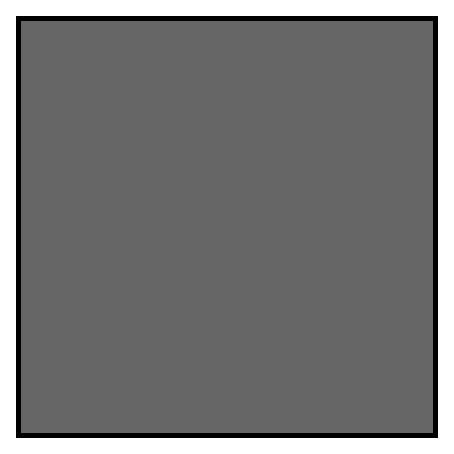
\includegraphics{example.eps}
%% figure caption is below the figure
%\caption{Please write your figure caption here}
%\label{fig:1}       % Give a unique label
%\end{figure}
%%
%% For two-column wide figures use
%\begin{figure*}
%% Use the relevant command to insert your figure file.
%% For example, with the graphicx package use
%  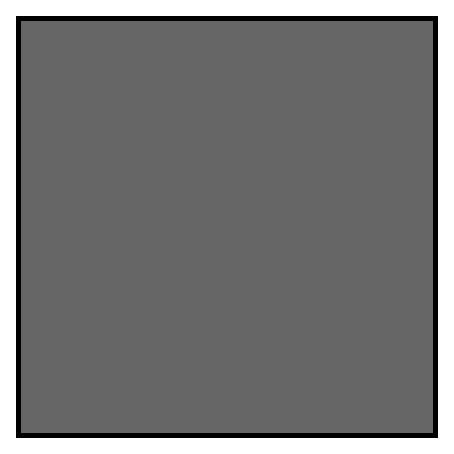
\includegraphics[width=0.75\textwidth]{example.eps}
%% figure caption is below the figure
%\caption{Please write your figure caption here}
%\label{fig:2}       % Give a unique label
%\end{figure*}
%%
%% For tables use
%\begin{table}
%% table caption is above the table
%\caption{Please write your table caption here}
%\label{tab:1}       % Give a unique label
%% For LaTeX tables use
%\begin{tabular}{lll}
%\hline\noalign{\smallskip}
%first & second & third  \\
%\noalign{\smallskip}\hline\noalign{\smallskip}
%number & number & number \\
%number & number & number \\
%\noalign{\smallskip}\hline
%\end{tabular}
%\end{table}


%\begin{acknowledgements}
%If you'd like to thank anyone, place your comments here
%and remove the percent signs.
%\end{acknowledgements}

% BibTeX users please use one of
%\bibliographystyle{spbasic}      % basic style, author-year citations
%\bibliographystyle{spmpsci}      % mathematics and physical sciences
%\bibliographystyle{spphys}       % APS-like style for physics
%\bibliography{}   % name your BibTeX data base



\end{document}
% end of file template.tex

